%definira klasu dokumenta 
\documentclass[12pt]{report} 

%prostor izmedu naredbi \documentclass i \begin{document} se zove uvod. U njemu se nalaze naredbe koje se odnose na cijeli dokument

%osnovni LaTex ne može riješiti sve probleme, pa se koriste različiti paketi koji olakšavaju izradu željenog dokumenta
\usepackage[croatian]{babel} 
\usepackage{amssymb}
\usepackage{amsmath}
\usepackage{txfonts}
\usepackage{mathdots}
\usepackage{titlesec}
\usepackage{array}
\usepackage{lastpage}
\usepackage{etoolbox}
\usepackage{tabularray}
\usepackage{color, colortbl}
\usepackage{adjustbox}
\usepackage{geometry}
\usepackage[classicReIm]{kpfonts}
\usepackage{hyperref}
\usepackage{fancyhdr}

\usepackage{float}
\usepackage{setspace}
\restylefloat{table}


\patchcmd{\chapter}{\thispagestyle{plain}}{\thispagestyle{fancy}}{}{} %redefiniranje stila stranice u paketu fancyhdr

%oblik naslova poglavlja
\titleformat{\chapter}{\normalfont\huge\bfseries}{\thechapter.}{20pt}{\Huge}
\titlespacing{\chapter}{0pt}{0pt}{40pt}


\linespread{1.3} %razmak između redaka

\geometry{a4paper, left=1in, top=1in,}  %oblik stranice

\hypersetup{ colorlinks, citecolor=black, filecolor=black, linkcolor=black,	urlcolor=black }   %izgled poveznice


%prored smanjen između redaka u nabrajanjima i popisima
\newenvironment{packed_enum}{
	\begin{enumerate}
		\setlength{\itemsep}{0pt}
		\setlength{\parskip}{0pt}
		\setlength{\parsep}{0pt}
	}{\end{enumerate}}

\newenvironment{packed_item}{
	\begin{itemize}
		\setlength{\itemsep}{0pt}
		\setlength{\parskip}{0pt}
		\setlength{\parsep}{0pt}
	}{\end{itemize}}




%boja za privatni i udaljeni kljuc u tablicama
\definecolor{LightBlue}{rgb}{0.9,0.9,1}
\definecolor{LightGreen}{rgb}{0.9,1,0.9}

%Promjena teksta za dugačke tablice
\DefTblrTemplate{contfoot-text}{normal}{Nastavljeno na idućoj stranici}
\SetTblrTemplate{contfoot-text}{normal}
\DefTblrTemplate{conthead-text}{normal}{(Nastavljeno)}
\SetTblrTemplate{conthead-text}{normal}
\DefTblrTemplate{middlehead,lasthead}{normal}{Nastavljeno od prethodne stranice}
\SetTblrTemplate{middlehead,lasthead}{normal}

%podesavanje zaglavlja i podnožja

\pagestyle{fancy}
\lhead{Programsko inženjerstvo}
\rhead{Sinappsa}
\lfoot{BijeliCasio}
\cfoot{stranica \thepage/\pageref{LastPage}}
\rfoot{\today}
\renewcommand{\headrulewidth}{0.2pt}
\renewcommand{\footrulewidth}{0.2pt}


\begin{document} 
	
	
	
	\begin{titlepage}
		\begin{center}
			\vspace*{\stretch{1.0}} %u kombinaciji s ostalim \vspace naredbama definira razmak između redaka teksta
			\LARGE Programsko inženjerstvo\\
			\large Ak. god. 2022./2023.\\
			
			\vspace*{\stretch{3.0}}
			
			\huge Sinappsa\\
			\Large Dokumentacija, Rev. 2.\\
			
			\vspace*{\stretch{12.0}}
			\normalsize
			Grupa: \textit{BijeliCasio}\\
			Voditelj: \textit{Borna Nikolić}\\
			
			
			\vspace*{\stretch{1.0}}
			Datum predaje: \textit{18.11.2022.}\\
	
			\vspace*{\stretch{4.0}}
			
			Nastavnik: \textit{Laura Majer}\\
		
		\end{center}

	
	\end{titlepage}

	
	\tableofcontents


	\chapter{Dnevnik promjena dokumentacije}	
		
		\begin{longtblr}[
				label=none
			]{
				width = \textwidth, 
				colspec={|X[2]|X[13]|X[3]|X[3]|}, 
				rowhead = 1
			}
			\hline
			\textbf{Rev.}	& \textbf{Opis promjene/dodatka} & \textbf{Autori} & \textbf{Datum}\\[3pt] \hline
			0.1 & Napravljen predložak	& Ana Grčević &  28.10.2022.		\\[3pt] \hline  
			0.2 & Dodan opis projektnog zadatka & Ana Grčević & 01.11.2022.  \\[3pt] \hline
			0.3 & Dodani obrasci uporabe & Ana Grčević, Martina Majdiš, Tin \newline Margetić, Borna Nikolić, Matija Pavičić, Mihael Petričević, Milica Vuković & 02.11.2022.  \\[3pt] \hline
			0.4 & Ispravak obrazaca uporabe & Ana Grčević & 10.11.2022.  \\[3pt]  \hline
			0.5 & Dodani sekvencijski dijagrami & Ana Grčević, Martina Majdiš, Tin \newline Margetić, Borna Nikolić, Matija Pavičić, Mihael Petričević, Milica Vuković & 10.11.2022.  \\[3pt]  \hline
			0.6 & Dodani dionici, aktori i funkcionalni zahtjevi & Ana Grčević & 13.11.2022.  \\[3pt]  \hline
			0.7 & Dodani ostali zahtjevi & Ana Grčević, Milica Vuković & 13.11.2022.  \\[3pt]  \hline
			0.8 & Dodani dijagram i opis baze podataka & Borna \newline Nikolić & 13.11.2022.  \\[3pt]  \hline
			0.9 & Dodan opis arhitekture sustava & Ana Grčević & 15.11.2022.  \\[3pt]  \hline
			0.10 & Dodan dijagram razreda & Ana Grčević, Borna Nikolić & 16.11.2022.  \\[3pt]  \hline
			\textbf{1.0} & Verzija samo s bitnim dijelovima za 1. ciklus &  &  \\[3pt] \hline 
			1.1 & Dodane korištene tehnologije i alati & Ana Grčević & 6.1.2023. \\[3pt] \hline  
			1.2 & Dodan dijagram stanja & Ana Grčević & 7.1.2023. \\[3pt] \hline
			1.3 & Dodane upute za puštanje u pogon & Ana Grčević, Borna Nikolić & 7.1.2023. \\[3pt] \hline
			1.4 & Dodan dijagram razmještaja & Ana Grčević & 7.1.2023. \\[3pt] \hline
			1.5 & Dodan dijagram aktivnosti & Ana Grčević & 7.1.2023. \\[3pt] \hline
			1.6 & Dodan dijagram komponenti & Borna \newline Nikolić & 7.1.2023. \\[3pt] \hline
			1.7 & Updejtan dijagram razreda & Borna \newline Nikolić & 7.1.2023. \\[3pt] \hline
			1.8 & Dodano ispitivanje programskog rješenja & Milica \newline Vuković & 9.1.2023. \\[3pt] \hline
			1.9 & Dodan zaključak & Ana Grčević & 9.1.2023. \\[3pt] \hline
			1.10 & Korigiranje teksta i provjera dokumentacije & Ana Grčević & 11.1.2023. \\[3pt] \hline
			\textbf{2.0} & Konačni tekst predloška dokumentacije  &  &  \\[3pt] \hline 
			&  &  & \\[3pt] \hline	
		\end{longtblr}
	
	\chapter{Opis projektnog zadatka}

			Sinappsa je web aplikacija koja omogućuje studentima FER-a da traže ili pružaju pomoć oko specifičnog gradiva, laboratorijskih vježbi ili kolegija općenito. Student-pomagač će moći staviti oglas na koji će se drugi studenti moći javljati. Nakon obavljenih instrukcija student daje recenziju studentu-pomagaču. Ta recenzija ulazi u cjelokupni rejting studenta koji se zatim prikazuje na rejting listi na web stranici. Prikaz rejting liste sadrži 10 registriranih članova s najvećim rejtingom i ažurira se redovito.
			
			Aplikacija se sastoji od tri vrste korisnika, a to su:
			\begin{packed_enum}
				\item neregistrirani korisnici
				\item registrirani korisnici 
				\item moderatori
			\end{packed_enum}
		
	\noindent \textbf{Neregistrirani korisnici}
	
			Neregistrirani korisnici na stranici vide objavljene oglase i rejting listu pod korisničkim imenom. Mogu filtrirati oglase po smjeru, kolegiju i kategoriji. Za smjer, padajući izbornik daje opcije elektrotehnika, računarstvo i nerazvrstani, a za kategoriju su moguće opcije laboratorijska vježba, blic, gradivo, kontinuirani ispit i ispitni rok.
			
			Ovim korisnicima nije dopušteno javljanje na oglase koje vide već se za tu mogućnost moraju registrirati službenom FER e-mail adresom. Opcija registracije ili prijave pojavljuje im se u padajućem izborniku klikom miša na ikonu u gornjem desnom kutu. Odabirom jedne od opcija, odlazi se na formu za registraciju ili prijavu.
			
			Već prije registrirani korisnik ima mogućnost prijave na svoj račun preko nadimka. Ako korisnik koji još nema račun završi na formi za prijavu, klikom na gumb „Nemaš račun?“ korisnik se preusmjerava na formu za registraciju. 
			
			Na formi za registraciju korisnik treba unijeti svoje ime, prezime, korisničko ime, avatara, e-mail i lozinku. Sustav provjerava pripada li e-mail adresa FER domeni. Nakon zahtjeva za registraciju, korisnik klikom na link u primljenom e-mail potvrđuje svoju registraciju.
			
			\begin{figure}[H]
				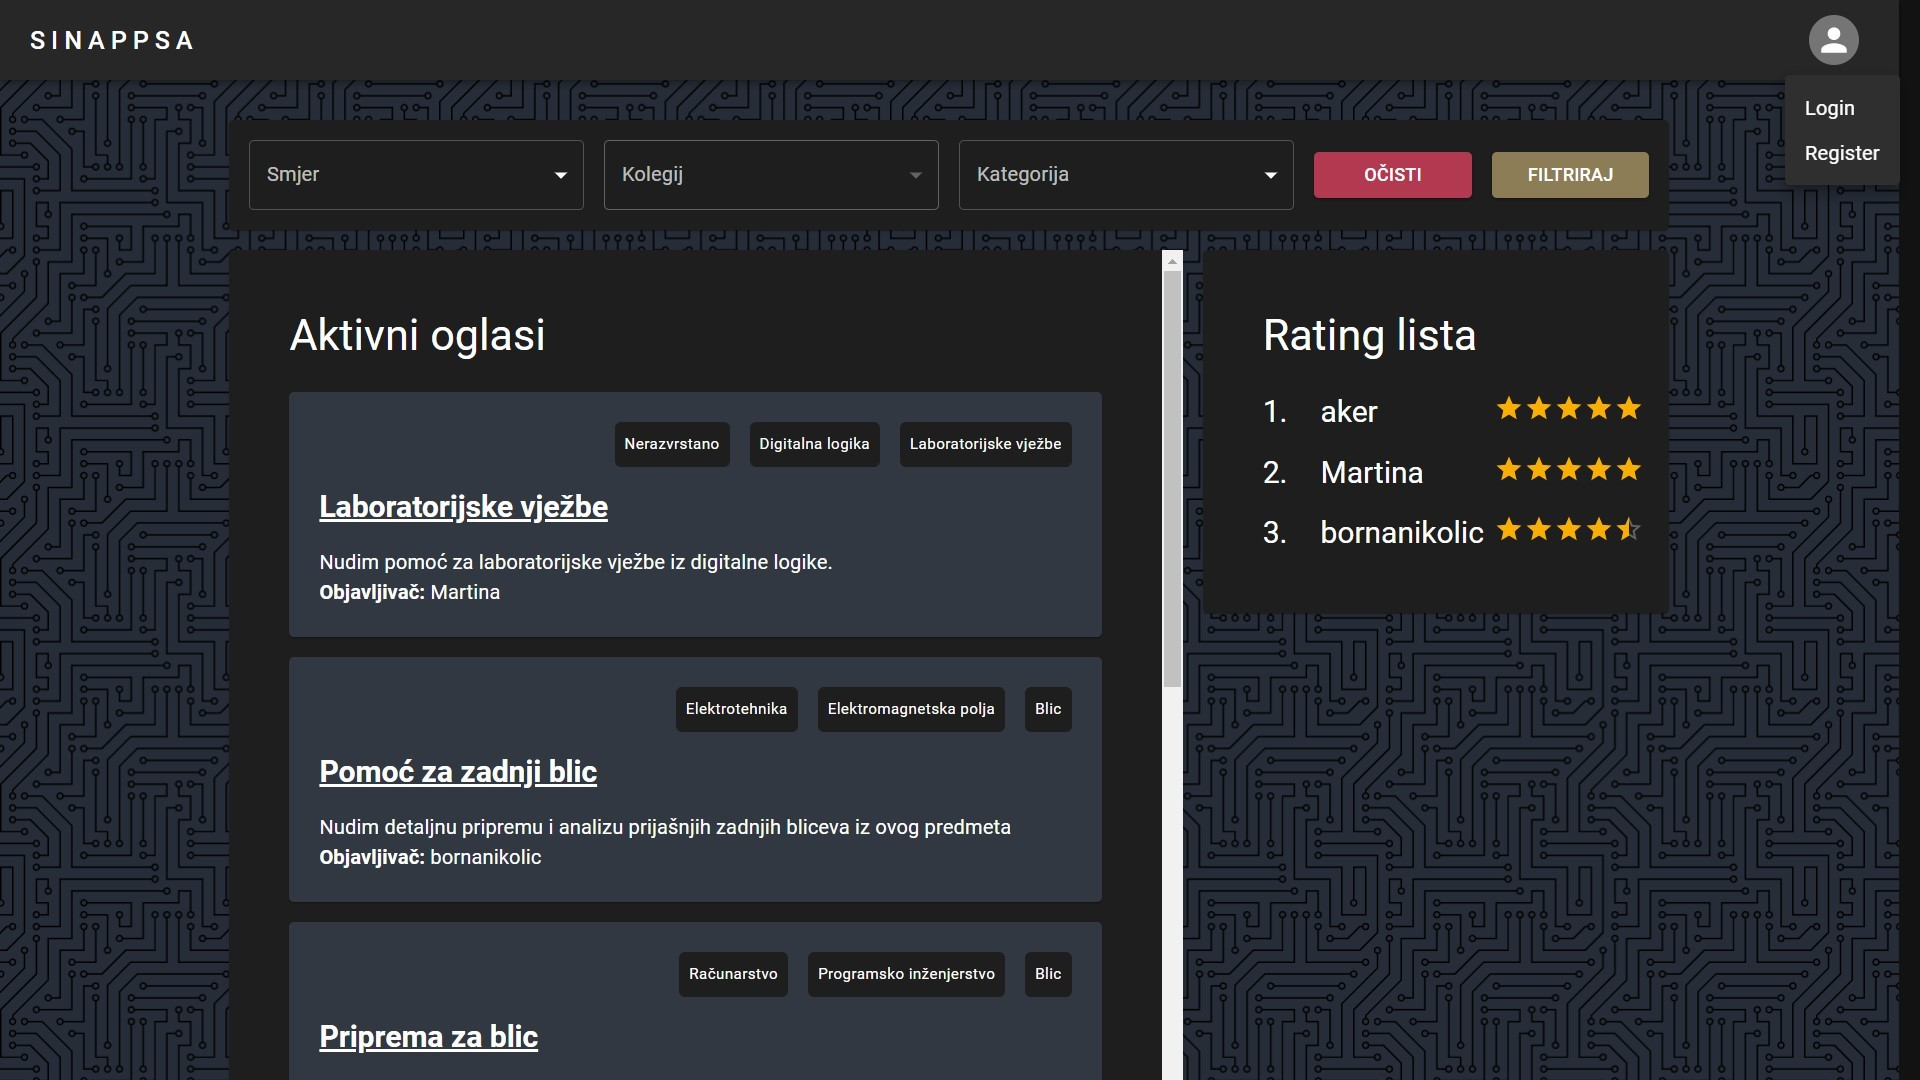
\includegraphics[scale=0.37]{slike/neregistrirani.jpg}
				\centering
				\caption{Početna stranica za neregistriranog korisnika}
				\label{fig:neregistriran}
			\end{figure} 
		
			\begin{figure}[H]
				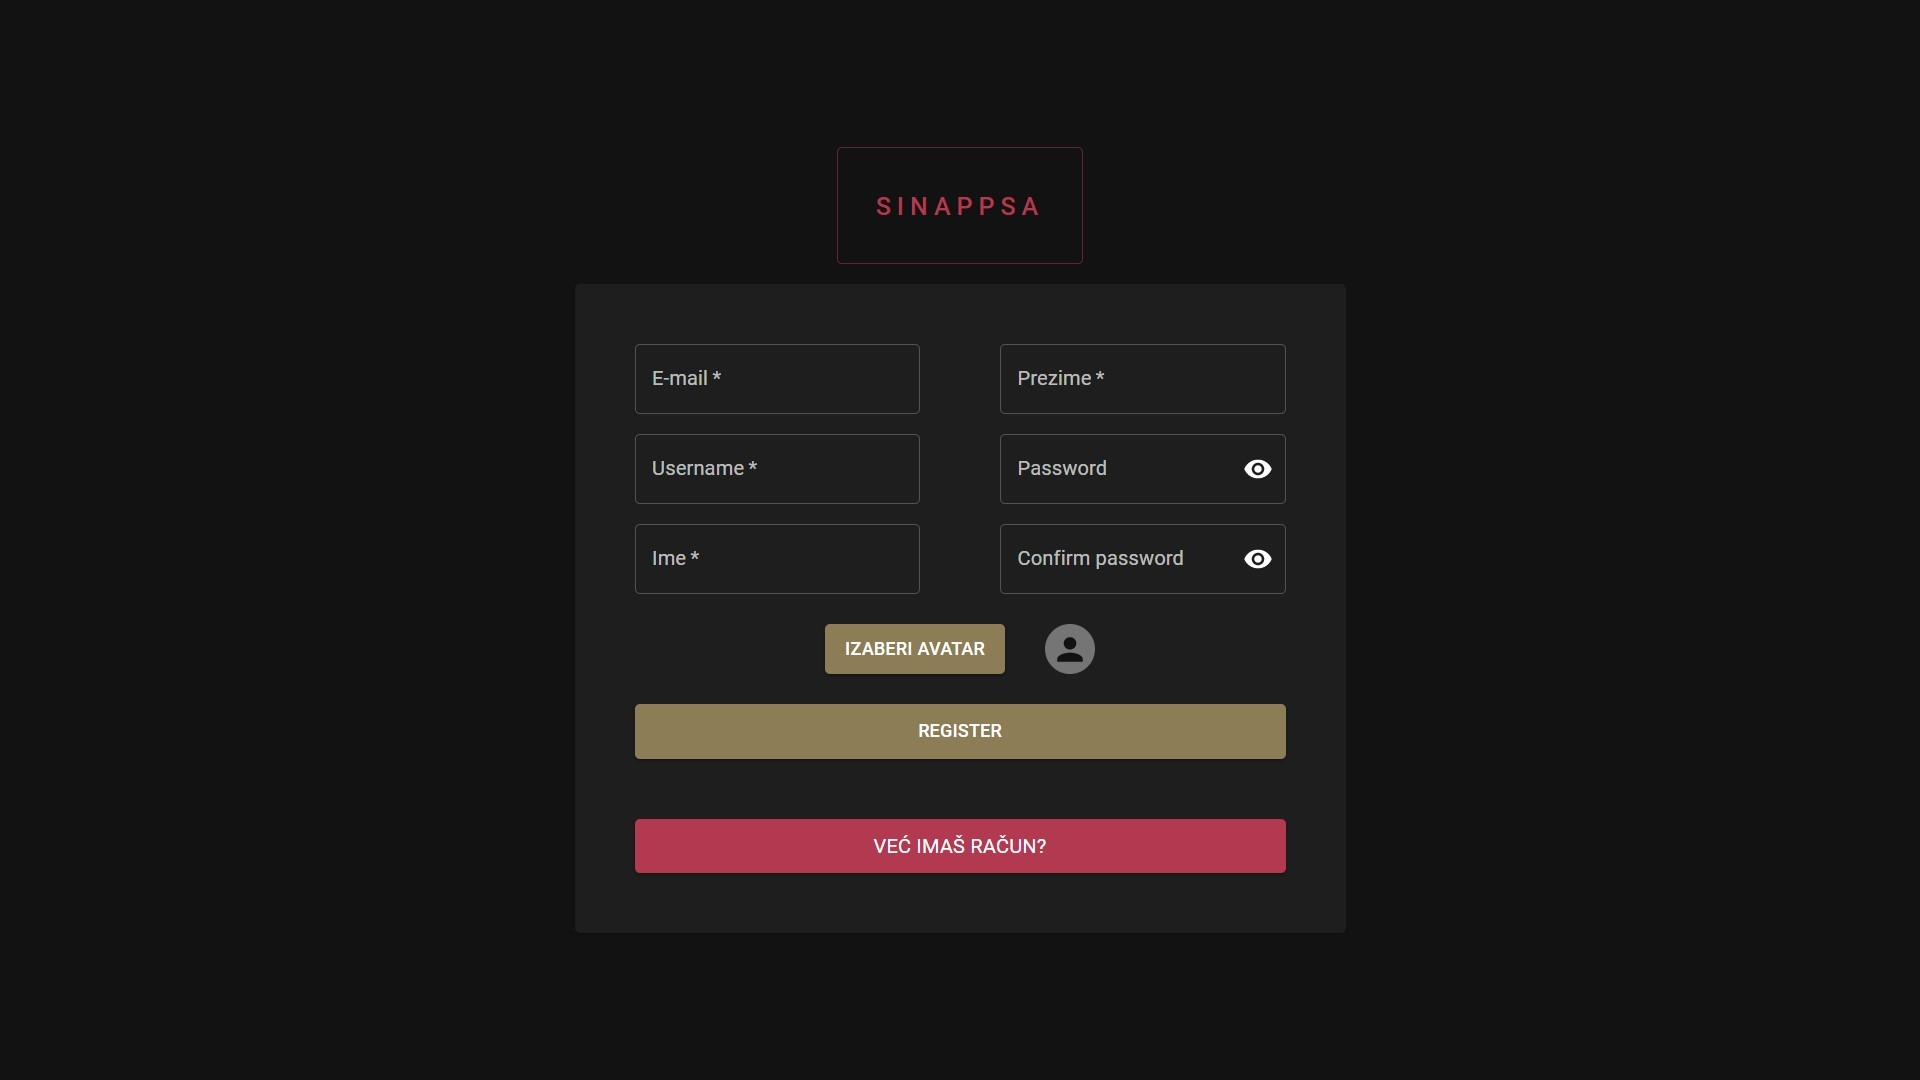
\includegraphics[scale=0.37]{slike/registracija.jpg} 
				\centering
				\caption{Forma za registraciju}
				\label{fig:registracija}
			\end{figure}
		
			\begin{figure}[H]
				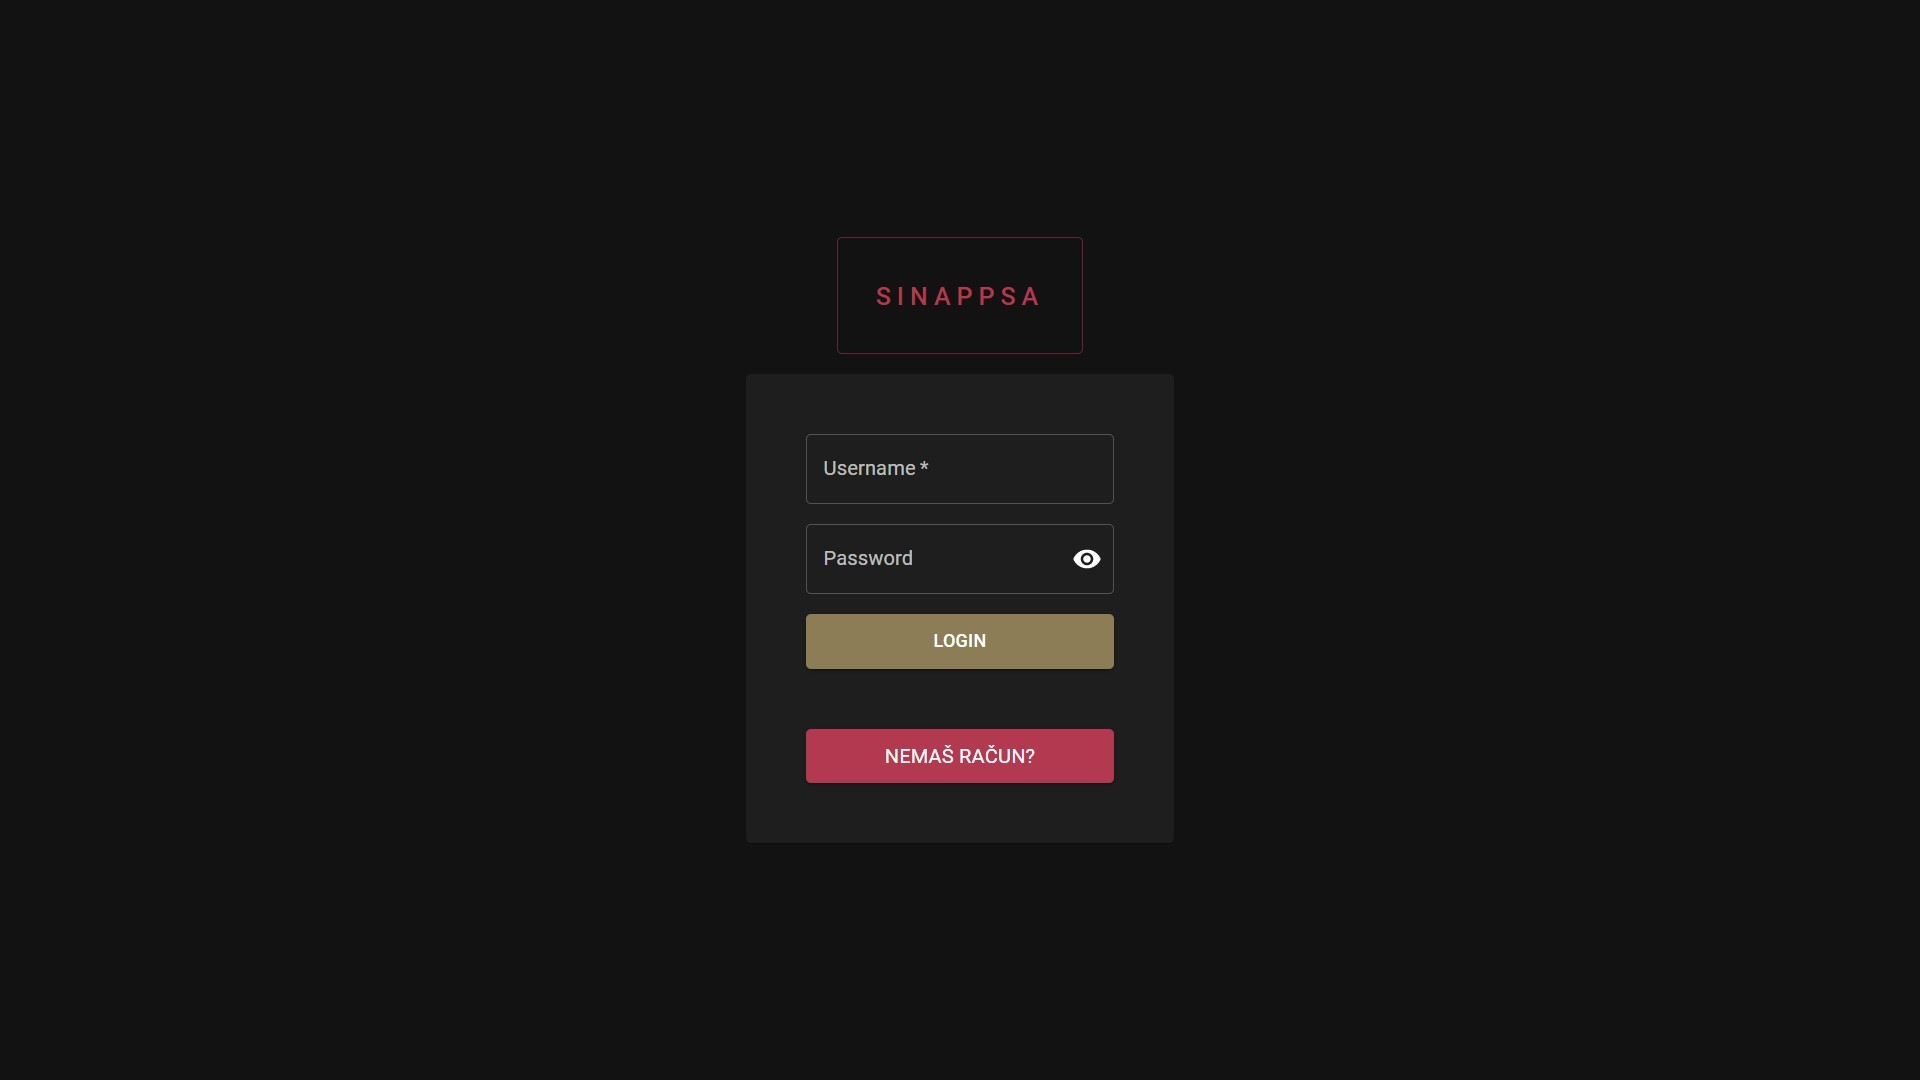
\includegraphics[scale=0.37]{slike/login.jpg} 
				\centering
				\caption{Forma za prijavu}
				\label{fig:prijava}
			\end{figure}
		
	\noindent \textbf{Registrirani korisnici}
	
			Registrirani korisnici, uz funkcionalnost neregistriranih korisnika, mogu objavljivati oglase i odgovarati na njih. Opcija stvaranja oglasa pojavljuje se u zaglavlju kao gumb „Dodaj oglas“. Pri stvaranju oglasa korisnik navodi naslov, opis, kolegij i kategoriju oglasa.
			
			Registrirani korisnici također mogu i odgovarati na oglase. Prilikom odgovora na oglas unosi se proizvoljna poruka koja se zajedno s kontakt informacijama korisnika šalje na e-mail adresu studentu-pomagaču. Daljnja komunikacija obavlja se preko e-maila. Upit na oglas može biti prihvaćen, odbijen ili u tijeku. Ako je korisnik dobio pozitivan odgovor, nakon odslušanih instrukcija, osoba ocjenjuje iste  te se ta ocjena pribraja u cjelokupni rejting studenta-pomagača. 
			
			\begin{figure}[H]
				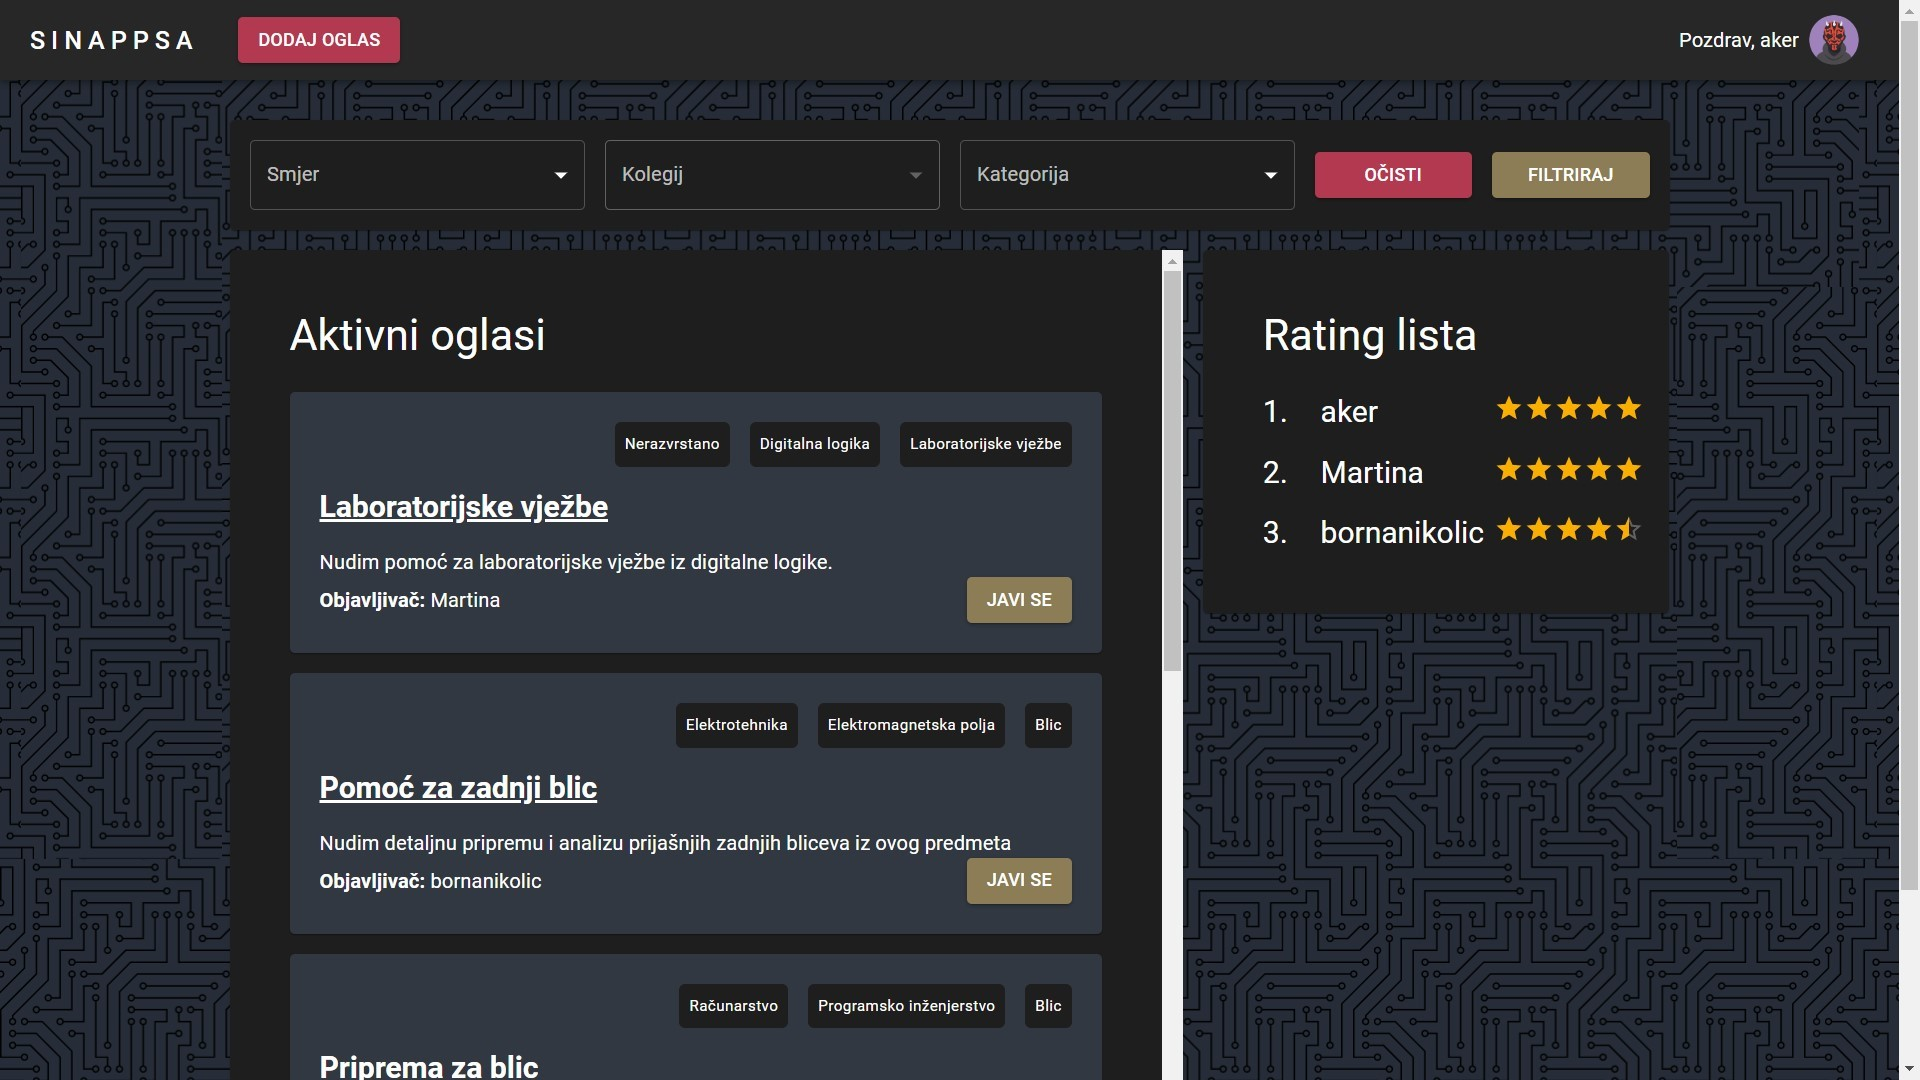
\includegraphics[scale=0.37]{slike/registrirani.jpg} 
				\centering
				\caption{Početna stranica za registriranog korisnika}
				\label{fig:registrirani}
			\end{figure}
		
			\begin{figure}[H]
				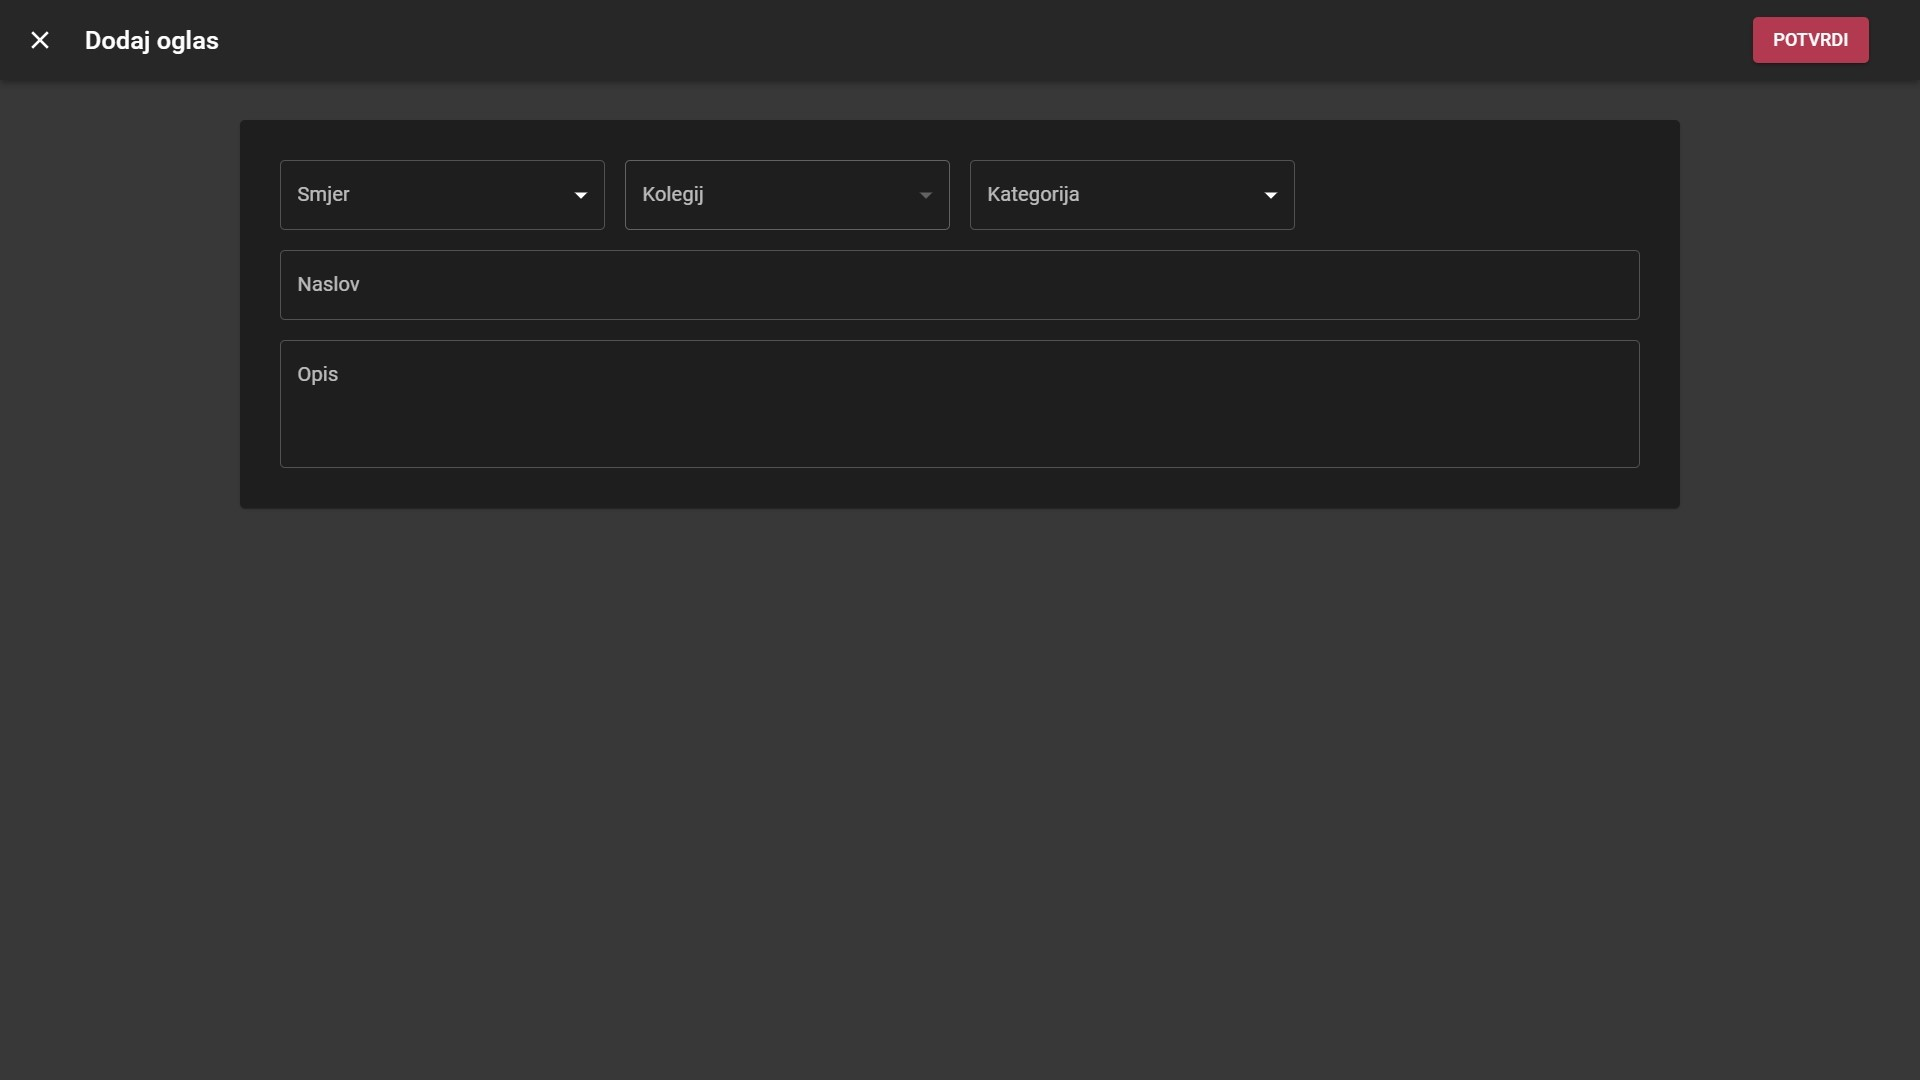
\includegraphics[scale=0.37]{slike/dodajOglas.jpg} 
				\centering
				\caption{Forma za dodavanje oglasa}
				\label{fig:oglas}
			\end{figure}
		
			Na svom profilu, korisniku se prikazuju njegovi aktivni oglasi, upiti na njegove oglase kao i statusi upita koje je korisnik poslao na druge oglase. Aktivnim oglasima može mijenjati naslov i opis te je u mogućnosti obrisati ih. Uz informacije o oglasima na profilu se nalaze i osobne informacije korisnika. Korisniku je omogućeno naknadno mijenjanje lozinke, korisničkog imena i avatara.
			
			\begin{figure}[H]
				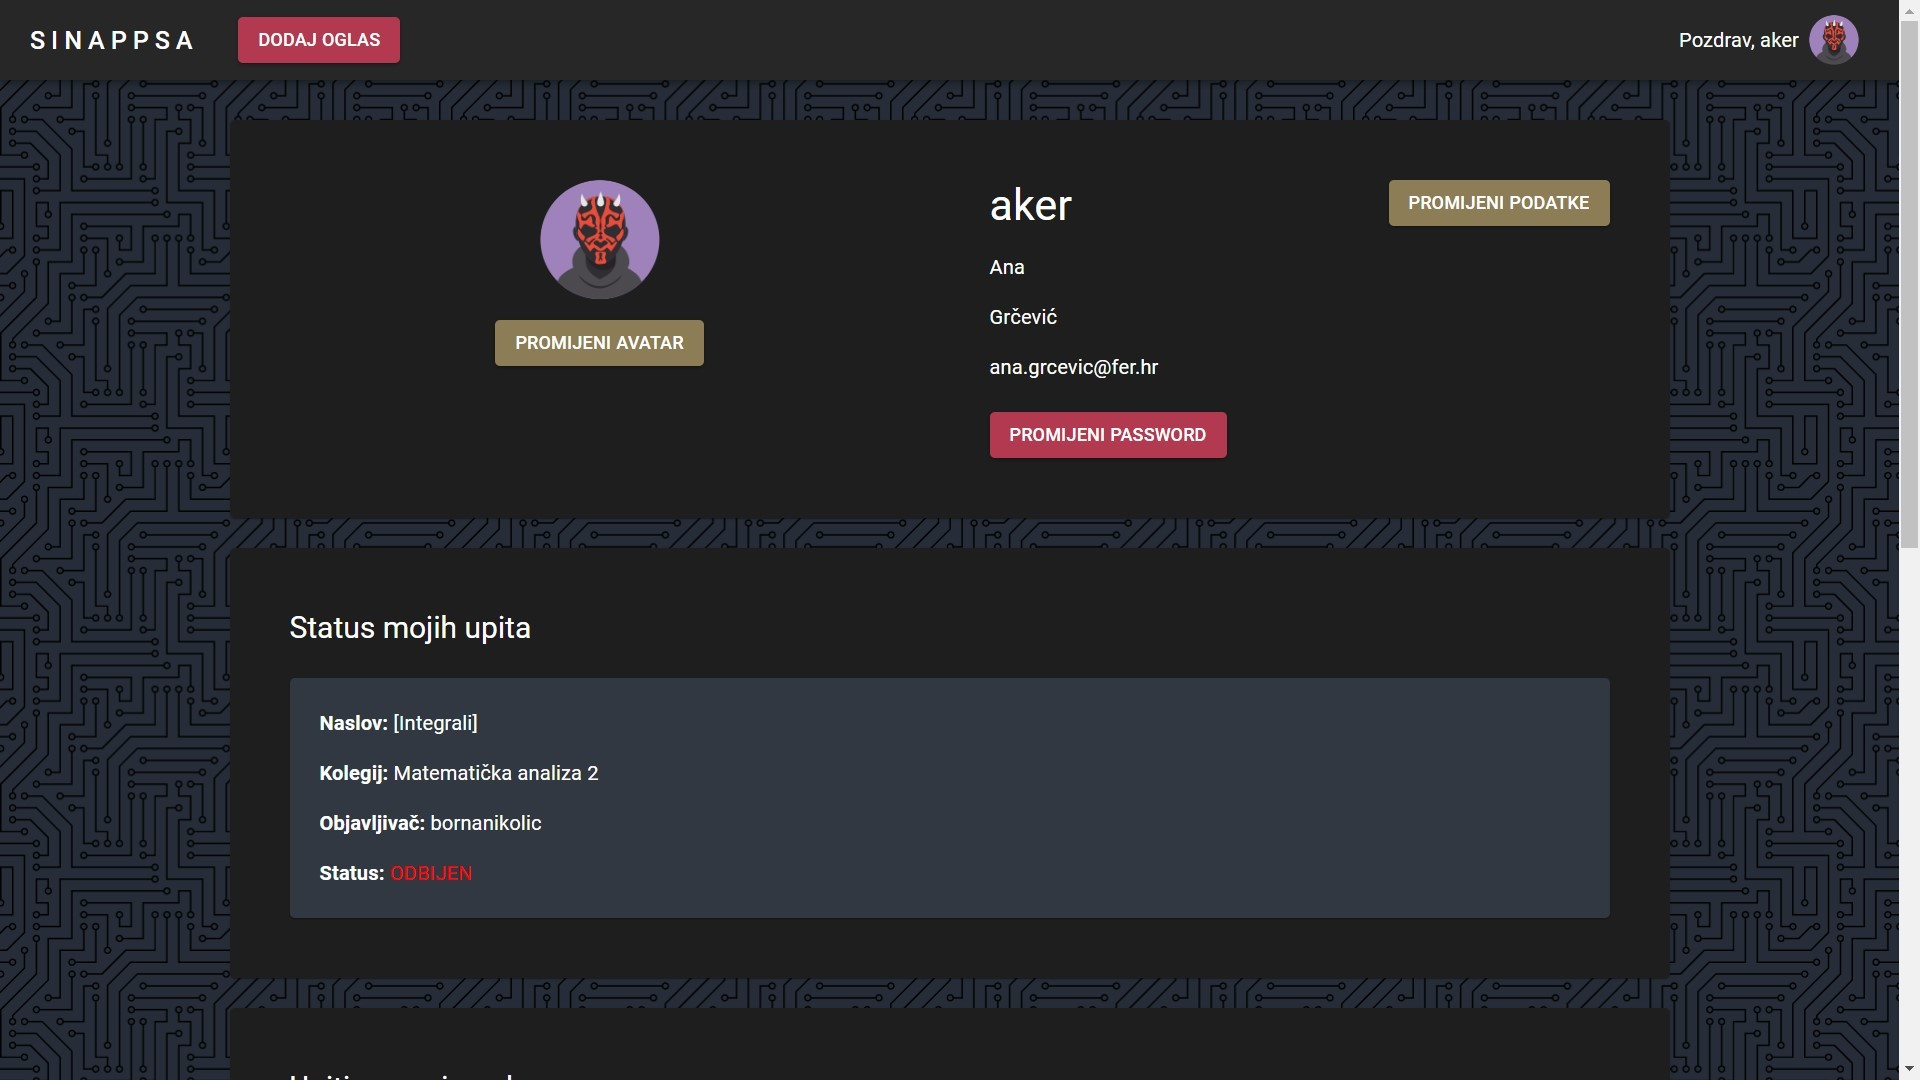
\includegraphics[scale=0.37]{slike/profil1.jpg} 
				\centering
				\caption{Izgled profila - prvi dio}
				\label{fig:profil1}
			\end{figure}
		
			\begin{figure}[H]
				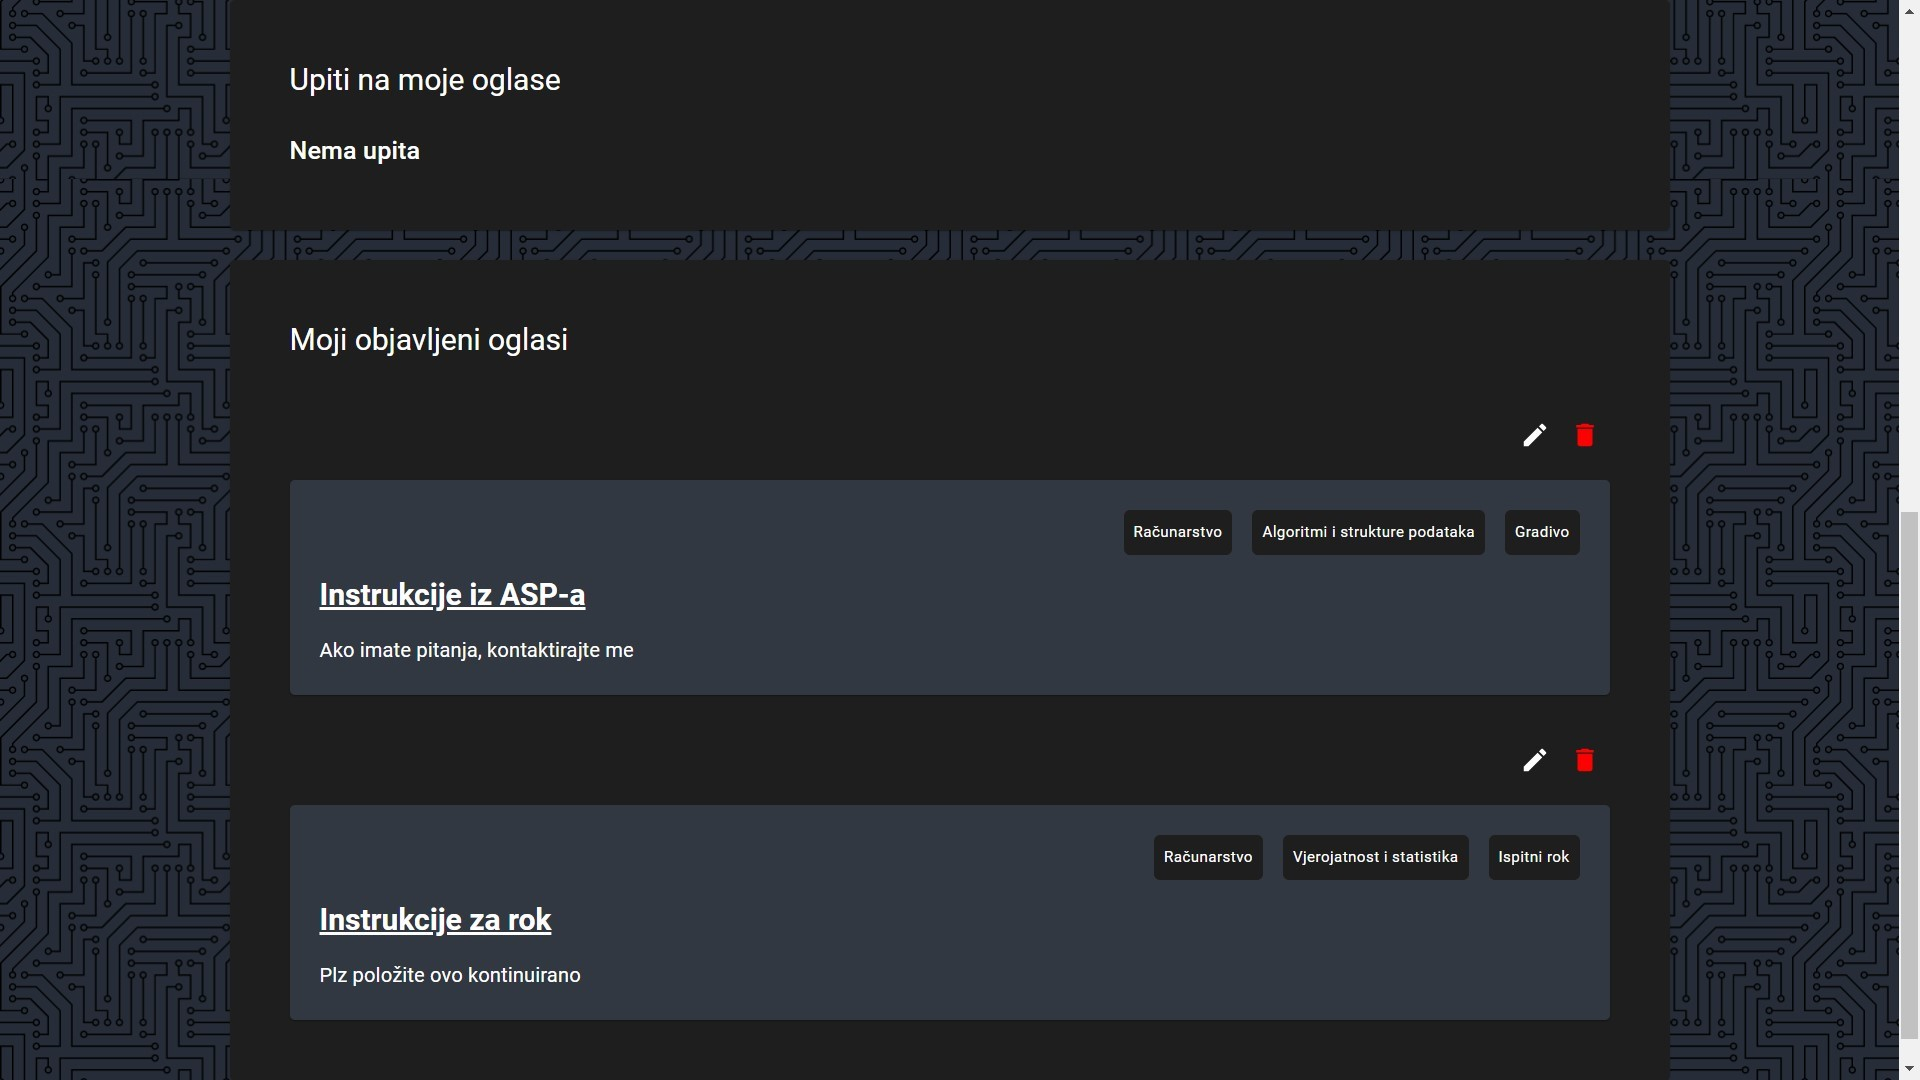
\includegraphics[scale=0.37]{slike/profil2.jpg} 
				\centering
				\caption{Izgled profila - drugi dio}
				\label{fig:profil2}
			\end{figure}
		
	\noindent \textbf{Moderator}
	
			Moderator ima ulogu uklanjanja nepravilnih ili neprikladnih oglasa. Kada moderator odabere opciju brisanja oglasa pojavljuje se skočni prozor u koji upisuje razlog zašto je oglas obrisan te se isti šalje na e-mail adresu objavljivaču oglasa. 
			
			Moderator također ima opciju dodavanja kolegija. Nakon odabira opcije „Dodaj kolegij“ koja se nalazi u zaglavlju, moderatoru se otvara skočni prozor gdje upisuje naziv kolegija koji želi dodati. Pored opcije "Dodaj kolegij" nalazi se gumb "Lista kolegija" čijim pritiskom se moderatoru prikazuje popis postojećih kolegija koje može uređivati, obrisati ili pretraživati.
			
			\begin{figure}[H]
				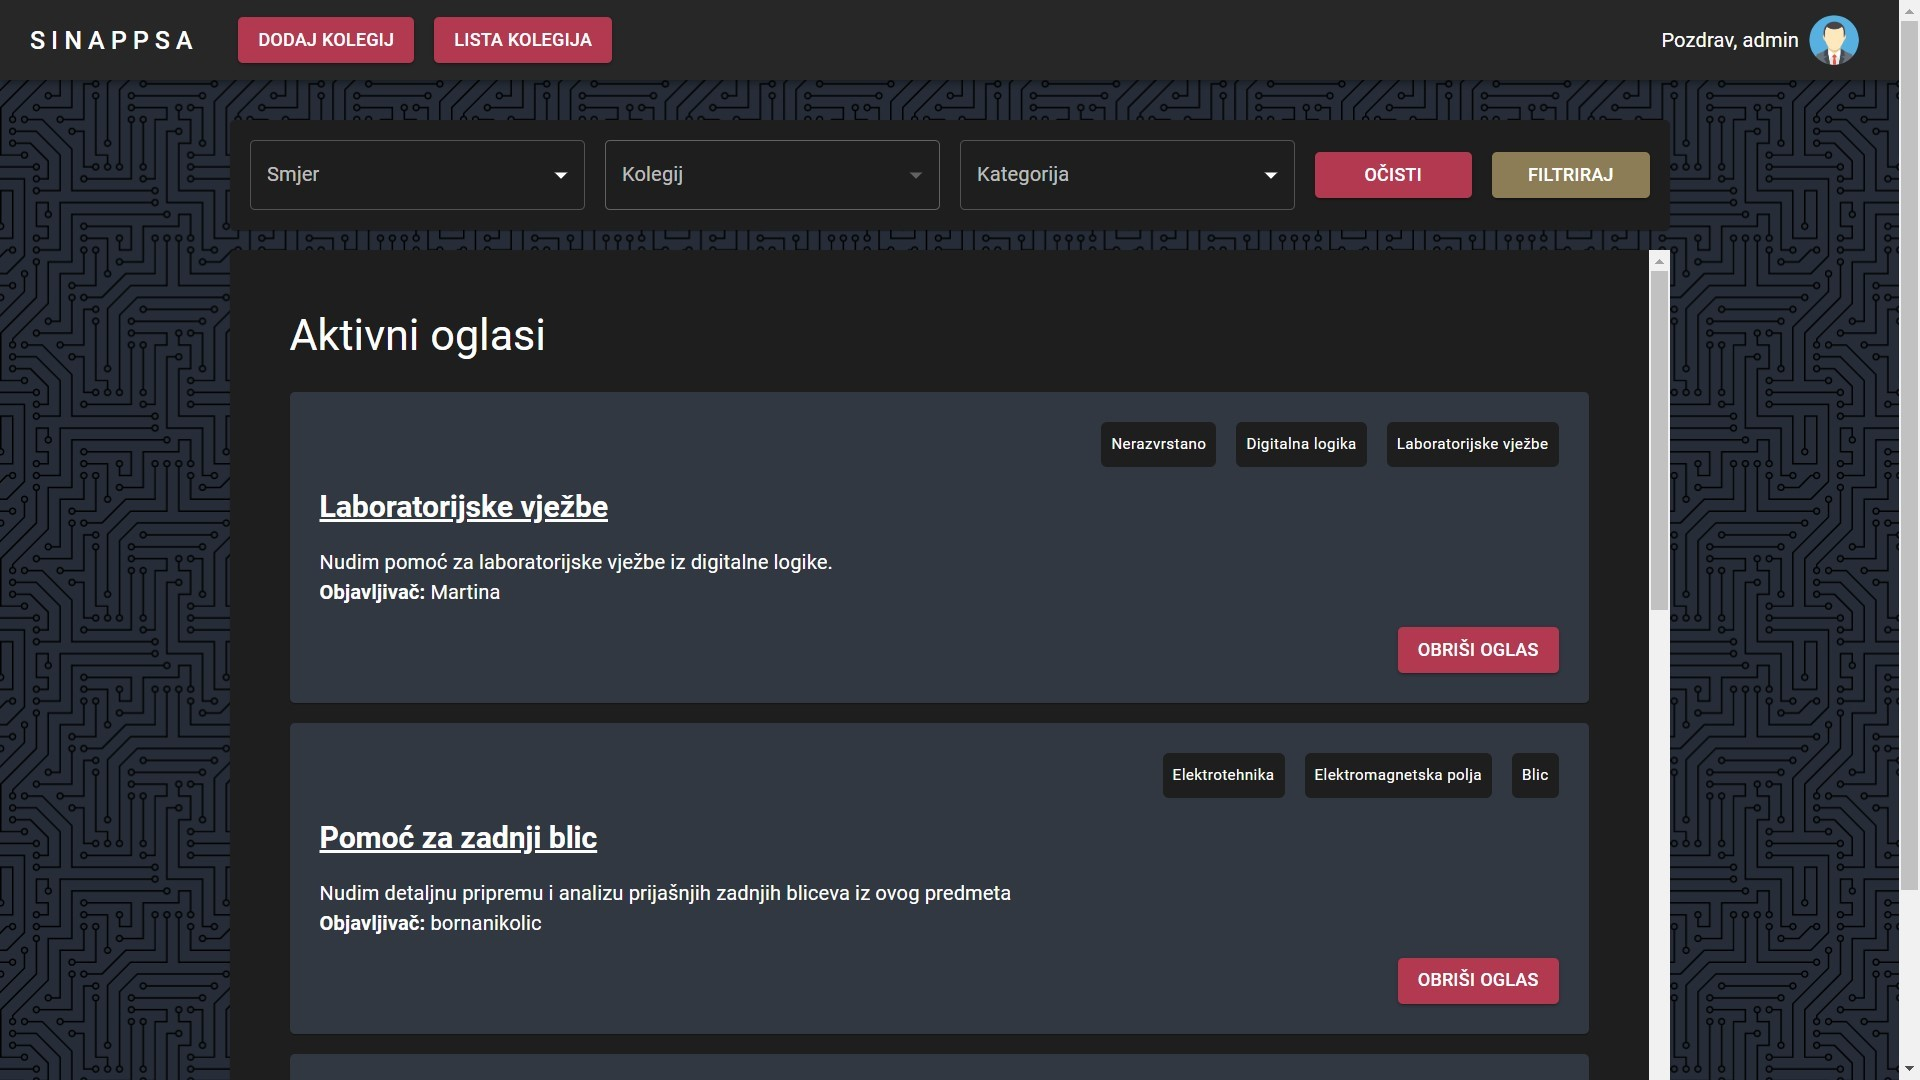
\includegraphics[scale=0.37]{slike/moderator1.jpg} 
				\centering
				\caption{Početna stranica za moderatora}
				\label{fig:moderator1}
			\end{figure}
		
			\begin{figure}[H]
				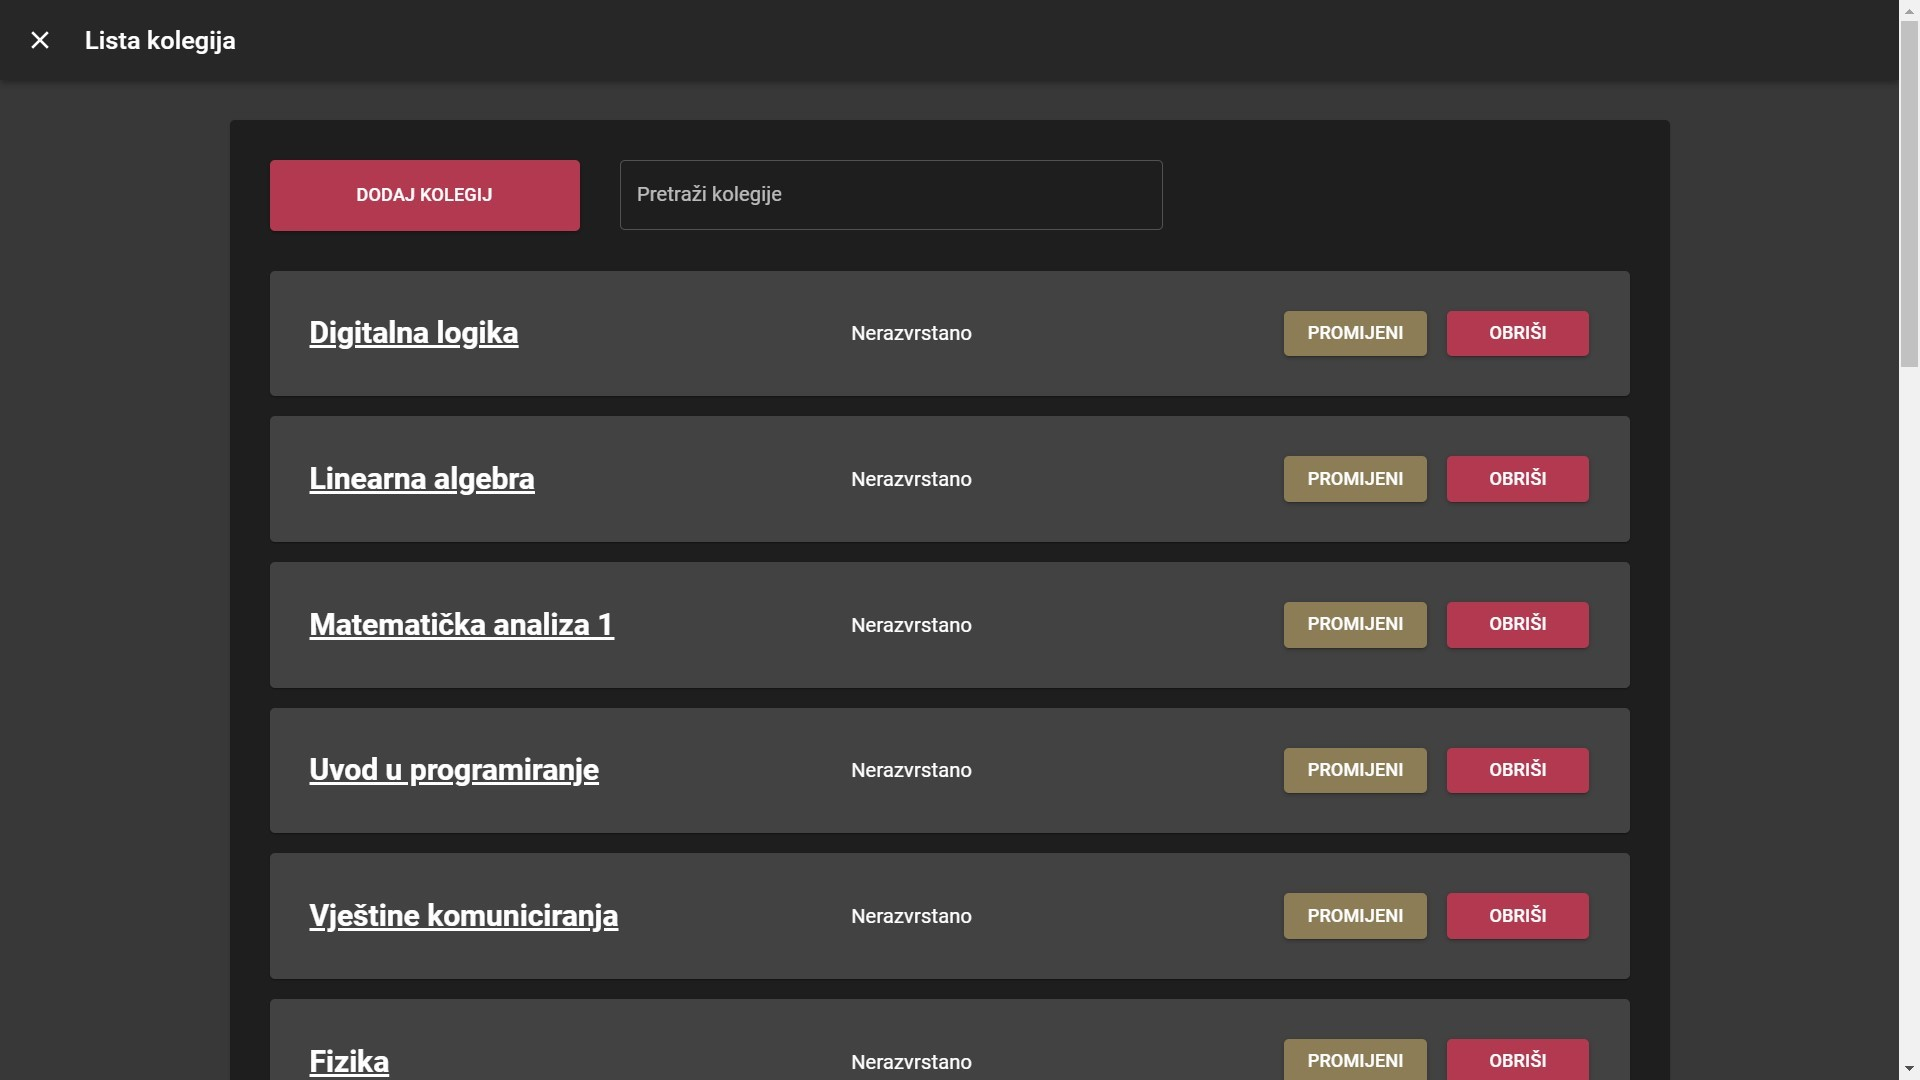
\includegraphics[scale=0.37]{slike/kolegiji.jpg} 
				\centering
				\caption{Lista dodanih kolegija}
				\label{fig:kolegiji}
			\end{figure}
		

		
		
	
	\chapter{Specifikacija programske potpore}
		
	\section{Funkcionalni zahtjevi}			
			
			\noindent \textbf{Dionici:}
			
			\begin{packed_enum}
				
				\item Korisnici
					\begin{packed_enum}
						\item  Neregistrirani
						\item  Registrirani
					\end{packed_enum}
				\item Moderator
				\item Razvojni tim
				
			\end{packed_enum}
			
			\noindent \textbf{Aktori i njihovi funkcionalni zahtjevi:}
			
			
			\begin{packed_enum}
				\item  \underbar{Neregistrirani/neprijavljeni korisnik (inicijator) može:}
				
				\begin{packed_enum}
					
					\item pregledati objavljene oglase pod nadimkom
					\item filtrirati oglase po smjeru, kolegiju i kategoriji
					\item pregledati rejting listu studenata- pomagača pod njihovim nadimkom
					\item se registrirati u sustav, stvoriti novi korisnički račun za koji su mu potrebni  ime, prezime, korisničko ime, avatara, e-mail i lozinka
					
				\end{packed_enum}
			
				\item  \underbar{Registrirani korisnik (inicijator) može:}
				
				\begin{packed_enum}
					
					\item javljati se na objavljene oglase
					\item objavljivati oglase
					\item ocjenjivati studente-pomagače
					\item pregledavati i mijenjati osobne podatke
					\item pregledavati i mijenjati svoje aktivne oglase
					\item obrisati svoje aktivne oglase
					\item promijeniti status upita na oglas (prihvaćen ili odbijen)
					
				\end{packed_enum}
			
				\item  \underbar{Moderator (inicijator) može:}
				
				\begin{packed_enum}
					
					\item uklanjati nepravilne i neprikladne oglase
					\item dodavati, mijenjati i brisati kolegije
					\item pretraživati kolegije
					
				\end{packed_enum}
			
				\item  \underbar{Baza podataka (sudionik):}
				
				\begin{packed_enum}
					
					\item pohranjuje sve podatke o korisnicima 
					\item pohranjuje sve podatke o oglasima
					\item pohranjuje kolegije
					
				\end{packed_enum}
			\end{packed_enum}
			
			\eject 
			
			
				
			\subsection{Obrasci uporabe}
				
				\subsubsection{Opis obrazaca uporabe}

					\noindent \underbar{\textbf{UC1 - Pregled objavljenih oglasa}}
					\begin{packed_item}
	
						\item \textbf{Glavni sudionik: }Neregistrirani korisnik
						\item  \textbf{Cilj:} Mogućnost pregleda objavljenih oglasa
						\item  \textbf{Sudionici:} Baza podataka
						\item  \textbf{Preduvjet:} -
						\item  \textbf{Opis osnovnog tijeka:}
						
						\item[] \begin{packed_enum}
							\item Dohvaćanje aktivnih oglasa iz baze podataka
							\item Prikaz aktivnih oglasa neregistriranom korisniku
						\end{packed_enum}
						
						\item  \textbf{Opis mogućih odstupanja:}
						
						\item[] \begin{packed_item}
	
							\item[1.a] Nema aktivnih oglasa
							\item[] \begin{packed_enum}
								\item Sustav obavještava korisnika da nema aktivnih oglasa
							\end{packed_enum}
							
						\end{packed_item}
					\end{packed_item}
				
				
					\noindent \underbar{\textbf{UC2 - Pregled rejting-liste}}
					\begin{packed_item}
						
						\item \textbf{Glavni sudionik: }Neregistrirani korisnik
						\item  \textbf{Cilj:} Mogućnost pregleda rejting-liste studenata pomagača pod nadimcima
						\item  \textbf{Sudionici:} Baza podataka
						\item  \textbf{Preduvjet:} -
						\item  \textbf{Opis osnovnog tijeka:}
						
						\item[] \begin{packed_enum}
							\item Neregistrirani korisnik zahtjeva prikaz liste 10 najboljih student-pomagača
							\item Lista student-pomagača dohvaća se iz baze podataka
							\item Rangiranje studenata-pomagača unutar web aplikacije
							\item Prikaz liste neregistriranom korisniku
						\end{packed_enum}
						
						\item  \textbf{Opis mogućih odstupanja:}
						
						\item[] \begin{packed_item}
							
							\item[2.a] Nema registriranih student-pomagača
							\item[] \begin{packed_enum}
								\item Sustav obavještava korisnika da ne postoje registrirani student-pomagači
							\end{packed_enum}
							
							\item[3.a] Studente-pomagače nije moguće rangirati
							\item[] \begin{packed_enum}
								\item Sustav prikazuje praznu rejting listu
							\end{packed_enum}
							
						\end{packed_item}
					\end{packed_item}
				
				
				
					\noindent \underbar{\textbf{UC3 - Filtriranje oglasa}}
					\begin{packed_item}
						
						\item \textbf{Glavni sudionik: }Neregistrirani korisnik
						\item  \textbf{Cilj:} Mogućnost filtriranja oglasa po smjeru, kolegiju i kategoriji
						\item  \textbf{Sudionici:} Baza podataka, Web aplikacija
						\item  \textbf{Preduvjet:} Korisniku se prikazuju aktivni oglasi
						\item  \textbf{Opis osnovnog tijeka:}
						
						\item[] \begin{packed_enum}
							\item Korisnik odabire opciju smjer(računarstvo ili elektrotehnika), kolegij i/ili kategoriju(laboratorijska vježba, blic, gradivo, kontinuirani ispit ili ispitni rok)
							\item Korisnik odabire opciju „Filtriraj“ 
							\item Web aplikacija filtrira listu oglasa po danim kriterijima i osvježava prikaz filtriranih oglasa
						\end{packed_enum}
						
						\item  \textbf{Opis mogućih odstupanja:}
						
						\item[] \begin{packed_item}
							
							\item[2.a] Korisnik filtrira, a nije izabrao nijednu od opcija (smjer, kolegij, kategorija):
							\item[] \begin{packed_enum}
								\item Prikazuju se svi oglasi
							\end{packed_enum}
							
						\end{packed_item}
					\end{packed_item}
				
					
					\noindent \underbar{\textbf{UC4 - Registracija}}
					\begin{packed_item}
						
						\item \textbf{Glavni sudionik: }Neregistrirani korisnik
						\item  \textbf{Cilj:} Stvoriti korisnički račun za pristup sustavu
						\item  \textbf{Sudionici:} Baza podataka
						\item  \textbf{Preduvjet:} -
						\item  \textbf{Opis osnovnog tijeka:}
						
						\item[] \begin{packed_enum}
							\item Korisnik odabire opciju za registraciju
							\item Korisnik unosi podatke potrebne za registraciju
							\item Aplikacija provjerava ispravni format unesenih podataka
							\item Podaci se upisuju u bazu podataka
							\item Korisniku se šalje e-mail pošta za potvrdu registracije računa
						\end{packed_enum}
						
						\item  \textbf{Opis mogućih odstupanja:}
						
						\item[] \begin{packed_item}
							
							\item[2.a] Korisnik je unio već zauzeto korisničko ime i/ili e-mail ili je unio e-mail koji nije iz fer.hr domene 
							\item[] \begin{packed_enum}
								\item Sustav obavještava korisnika o pogrešci te briše polje lozinke
							\end{packed_enum}

						\end{packed_item}
					\end{packed_item}
				
	
				
				\noindent \underbar{\textbf{UC5 - Pregled svojih objavljenih oglasa}}
				\begin{packed_item}
					
					\item \textbf{Glavni sudionik: }Registrirani korisnik
					\item  \textbf{Cilj:} Pregledati sve svoje objavljene oglase  
					\item  \textbf{Sudionici:} Baza podataka
					\item  \textbf{Preduvjet:} Korisnik je prijavljen
					\item  \textbf{Opis osnovnog tijeka:}
					
					\item[] \begin{packed_enum}
						\item Korisnik odlazi na rubriku „Moji objavljeni oglasi“
						\item Aplikacija šalje upit bazi za prikaz svih aktivnih oglasa
						\item Aktivni oglasi prikazuju se korisniku
					\end{packed_enum}
					
					\item  \textbf{Opis mogućih odstupanja:}
					
					\item[] \begin{packed_item}
						
						\item[2.a] Nema aktivnih oglasa za prikaz
						\item[] \begin{packed_enum}
							\item Aplikacija ispisuje poruku „Nema oglasa za prikaz“ 
						\end{packed_enum}
						
					\end{packed_item}
				\end{packed_item}
				
				
					\noindent \underbar{\textbf{UC6 - Objava oglasa }}
					\begin{packed_item}
						
						\item \textbf{Glavni sudionik: }Registrirani korisnik
						\item  \textbf{Cilj:} Objaviti oglas  
						\item  \textbf{Sudionici:} Baza podataka
						\item  \textbf{Preduvjet:} Korisnik je prijavljen
						\item  \textbf{Opis osnovnog tijeka:}
						
						\item[] \begin{packed_enum}
							\item Korisnik odabire opciju „Objavi oglas“
							\item Unosi sadržaj svog oglasa (naslov, opis, kolegij, kategorija) 
							\item Podaci se upisuju u bazu podataka
						\end{packed_enum}
						
						\item  \textbf{Opis mogućih odstupanja:}
						
						\item[] \begin{packed_item}
							
							\item[2.a] Korisnik nije unio sve obvezne komponente oglasa
							\item[] \begin{packed_enum}
								\item Sustav obavještava korisnika o podacima koji nisu ispravno uneseni
							\end{packed_enum}
							
						\end{packed_item}
					\end{packed_item}
				
				
					
				
				
					\noindent \underbar{\textbf{UC7 - Izmjena objavljenih oglasa}}
					\begin{packed_item}
						
						\item \textbf{Glavni sudionik: }Registrirani korisnik
						\item  \textbf{Cilj:} Izmijeniti značajke oglasa   
						\item  \textbf{Sudionici:} Baza podataka
						\item  \textbf{Preduvjet:} Korisnik je prijavljen i oglas je objavljen
						\item  \textbf{Opis osnovnog tijeka:}
						
						\item[] \begin{packed_enum}
							\item Korisnik odlazi na rubriku „Moji objavljeni oglasi“
							\item Korisnik odabire oglas koji želi izmijeniti
							\item Korisnik odabere opciju za izmjenu oglasa
							\item Korisnik izmjenjuje željene značajke oglasa
							\item Korisnik sprema promjene
							\item Baza podataka se ažurira
						\end{packed_enum}
						
						\item  \textbf{Opis mogućih odstupanja:}
						
						\item[] \begin{packed_item}
							
							\item[4.a] Korisnik je obrisao sav sadržaj oglasa i pokušava ga ponovno objaviti 
							\item[] \begin{packed_enum}
								\item Sustav obavještava korisnika da ne može objaviti prazan oglas
							\end{packed_enum}
							
						\end{packed_item}
					\end{packed_item}
					
					
					\noindent \underbar{\textbf{UC8 - Brisanje oglasa}}
					\begin{packed_item}
						
						\item \textbf{Glavni sudionik: }Registrirani korisnik
						\item  \textbf{Cilj:} Obrisati objavljeni oglas  
						\item  \textbf{Sudionici:} Baza podataka
						\item  \textbf{Preduvjet:} Korisnik je prijavljen i oglas je objavljen
						\item  \textbf{Opis osnovnog tijeka:}
						
						\item[] \begin{packed_enum}
							\item Korisnik odlazi na rubriku „Moji objavljeni oglasi“
							\item Korisnik odabire oglas koji želi obrisati
							\item Korisnik stisne gumb „Obriši oglas“
							\item Sustav izbacuje skočni prozor s pitanjem „Jeste li sigurni da želite obrisati ovaj oglas?“
							\item Korisnik odabire „Da“ ili „Ne“
							\item Baza podataka se ažurira
						\end{packed_enum}
						
					\end{packed_item}
				
				
					\noindent \underbar{\textbf{UC9 - Odgovaranje na oglase}}
					\begin{packed_item}
						
						\item \textbf{Glavni sudionik: }Registrirani korisnik
						\item  \textbf{Cilj:} Odgovoriti na objavljeni oglas   
						\item  \textbf{Sudionici:} Baza podataka
						\item  \textbf{Preduvjet:} Korisnik je prijavljen i oglas je objavljen
						\item  \textbf{Opis osnovnog tijeka:}
						
						\item[] \begin{packed_enum}
							\item Korisnik bira oglas na koji želi odgovoriti
							\item Korisnik upisuje svoj odgovor
							\item Sustav šalje e-mail objavljivaču oglasa
							\item Daljnja komunikacija odvija se e-mailom između korisnika i studenta-pomagača
						\end{packed_enum}
						
					\end{packed_item}
				
				
					\noindent \underbar{\textbf{UC10 - Pregled statusa upita}}
					\begin{packed_item}
						
						\item \textbf{Glavni sudionik: }Registrirani korisnik
						\item  \textbf{Cilj:} Pogledati status poslanog upita  
						\item  \textbf{Sudionici:} Baza podataka
						\item  \textbf{Preduvjet:} Korisnik je prijavljen i poslan je upit na oglas
						\item  \textbf{Opis osnovnog tijeka:}
						
						\item[] \begin{packed_enum}
							\item Korisnik odlazi na rubriku „Status mojih upita“
							\item Aplikacija šalje upit bazi za prikaz statusa upita
							\item Korisniku se prikazuje status njegovog upita (prihvaćen, odbijen ili u tijeku)
						\end{packed_enum}
						
					\end{packed_item}
				
				
					\noindent \underbar{\textbf{UC11 - Promjena statusa upita}}
					\begin{packed_item}
						
						\item \textbf{Glavni sudionik: }Registrirani korisnik
						\item  \textbf{Cilj:} Promijeniti status primljenog upita  
						\item  \textbf{Sudionici:} Baza podataka
						\item  \textbf{Preduvjet:} Korisnik je prijavljen i primljen je upit na oglas
						\item  \textbf{Opis osnovnog tijeka:}
						
						\item[] \begin{packed_enum}
							\item Korisnik odlazi na rubriku „Upiti na moje oglase“
							\item Aplikacija šalje upit bazi za prikaz upita
							\item Korisniku se prikazuje upiti na njegove oglase
							\item Korisnik prihvaća ili odbija upit na oglas
							\item Baza podataka se ažurira
						\end{packed_enum}
						
					\end{packed_item}
				
				
					\noindent \underbar{\textbf{UC12 - Ocjenjivanje pomagača}}
					\begin{packed_item}
						
						\item \textbf{Glavni sudionik: }Registrirani korisnik
						\item  \textbf{Cilj:} Ocijeniti studenta-pomagača  
						\item  \textbf{Sudionici:} Baza podataka
						\item  \textbf{Preduvjet:} Korisnik je prijavljen i objavljen je bar jedan oglas na temelju kojeg se pomagač ocjenjuje
						\item  \textbf{Opis osnovnog tijeka:}
						
						\item[] \begin{packed_enum}
							\item Korisnik nakon pozitivnog odgovora ocjenjuje studenta-pomagača 
							\item Korisnik odabire ocjenu koju mu želi dati 
							\item Ažurira se rejting-lista i srednja ocjena studenta-pomagača
							\item Baza podataka se ažurira
						\end{packed_enum}
						
					\end{packed_item}
				
				
					\noindent \underbar{\textbf{UC13 - Izmjena informacija o profilu}}
					\begin{packed_item}
						
						\item \textbf{Glavni sudionik: }Registrirani korisnik
						\item  \textbf{Cilj:} Izmijeniti informacije o svom profilu 
						\item  \textbf{Sudionici:} Baza podataka
						\item  \textbf{Preduvjet:} Korisnik je prijavljen
						\item  \textbf{Opis osnovnog tijeka:}
						
						\item[] \begin{packed_enum}
							\item Korisnik odabire opciju za promjenu svojih podataka 
							\item Korisnik mijenja svoje podatke 
							\item Korisnik sprema promjene
							\item Baza podataka se ažurira
						\end{packed_enum}
					
					\end{packed_item}
				
				
					\noindent \underbar{\textbf{UC14 - Uklanjanje nepravilnih oglasa}}
					\begin{packed_item}
						
						\item \textbf{Glavni sudionik: }Moderator
						\item  \textbf{Cilj:} Ukloniti nepravilne ili neprikladne oglase
						\item  \textbf{Sudionici:} Baza podataka
						\item  \textbf{Preduvjet:} Korisnik je prijavljen i dodijeljena su mu prava moderatora
						\item  \textbf{Opis osnovnog tijeka:}
						
						\item[] \begin{packed_enum}
							\item Moderator pregledava oglase i utvrđuje nepravilnosti
							\item Moderator piše objašnjenje za brisanje oglasa 
							\item Moderator odabire opciju „Obriši oglas”
							\item Korisniku se šalje e-mail s objašnjenjem zašto je njegov oglas uklonjen
							\item Baza podataka se ažurira
							
						\end{packed_enum}
						
						\item  \textbf{Opis mogućih odstupanja:}
						
						\item[] \begin{packed_item}
							
							\item[1.a] Nema aktivnih oglasa
							\item[] \begin{packed_enum}
								\item Sustav obavještava moderatora da nema aktivnih oglasa
							\end{packed_enum}
							
						\end{packed_item}
					\end{packed_item}
				
				
					\noindent \underbar{\textbf{UC15 - Dodavanje kolegija}}
					\begin{packed_item}
						
						\item \textbf{Glavni sudionik: }Moderator
						\item  \textbf{Cilj:} Dodati novi kolegij
						\item  \textbf{Sudionici:} Baza podataka
						\item  \textbf{Preduvjet:} Korisnik je prijavljen i dodijeljena su mu prava moderatora
						\item  \textbf{Opis osnovnog tijeka:}
						
						\item[] \begin{packed_enum}
							\item Moderator odabire opciju „Dodaj kolegija”
							\item Moderator unosi podatke o novom kolegiju  
							\item Moderator odabire opciju „Unesi kolegij”
							\item Podaci se upisuju u bazu podataka
							
						\end{packed_enum}
						
						\item  \textbf{Opis mogućih odstupanja:}
						
						\item[] \begin{packed_item}
							
							\item[3.a] Kolegij već postoji u bazi podataka
							\item[] \begin{packed_enum}
								\item Sustav obavještava moderatora o neuspješnom unosu kolegija u bazu podataka
							\end{packed_enum}
							
						\end{packed_item}
					\end{packed_item}
				
				
					\noindent \underbar{\textbf{UC16 - Kategorizacija kolegija}}
					\begin{packed_item}
						
						\item \textbf{Glavni sudionik: }Moderator
						\item  \textbf{Cilj:} Kategorizirati kolegij po smjerovima
						\item  \textbf{Sudionici:} Baza podataka
						\item  \textbf{Preduvjet:} Korisnik je prijavljen i dodijeljena su mu prava moderatora, kolegij postoji u bazi podataka
						\item  \textbf{Opis osnovnog tijeka:}
						
						\item[] \begin{packed_enum}
							\item Moderator odabire prikaz liste kolegija
							\item Moderator odabire kolegij iz liste kolegija 
							\item Moderator odabire smjer (jedan od preddiplomskih ili diplomskih smjerova)
							\item Podaci se upisuju u bazu podataka
							
						\end{packed_enum}
						
					\end{packed_item}
				
				\eject
					
				\subsubsection{Dijagrami obrazaca uporabe}
				
					\begin{figure}[H]
						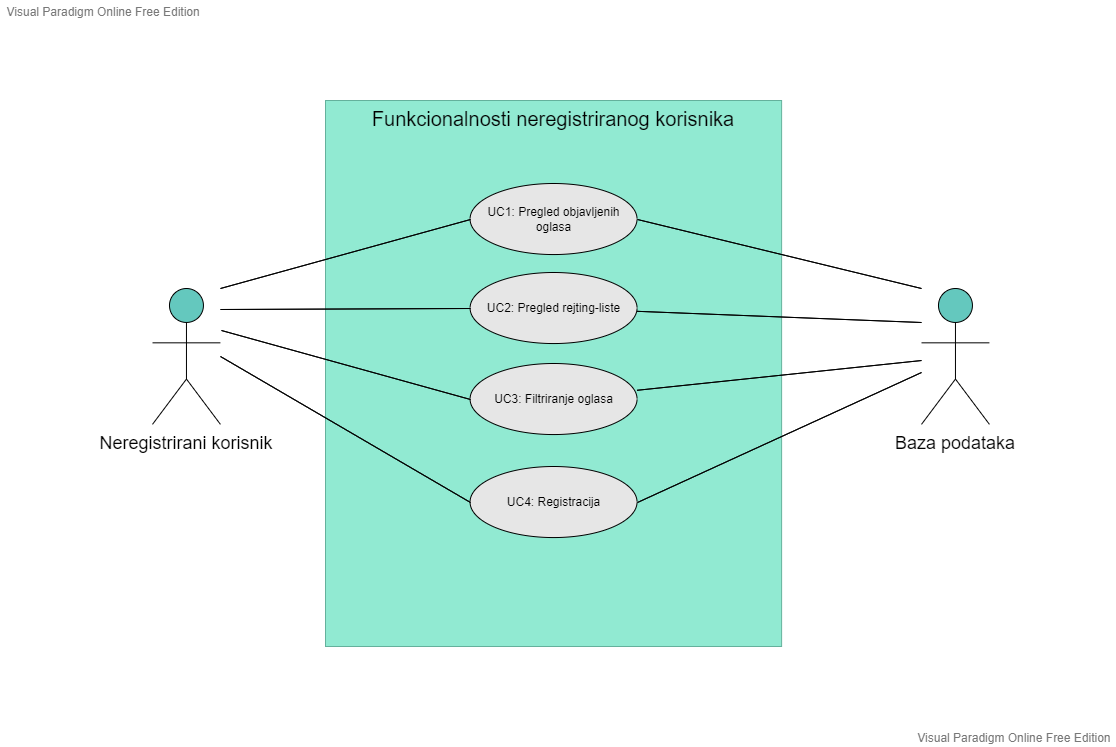
\includegraphics[scale=0.63]{dijagrami/UC_NeregistriranKorisnik.PNG}
						\centering
						\caption{Dijagram obrasca uporabe, funkcionalnosti neregistriranog korisnika}
						\label{fig:UC_NeregistriranKorisnik}
					\end{figure}
				
					\begin{figure}[H]
						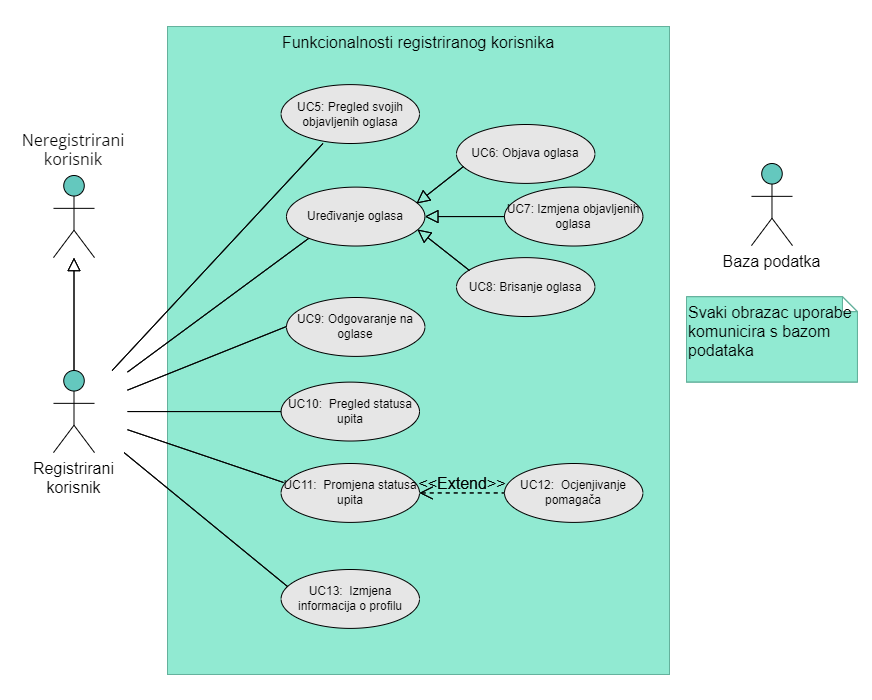
\includegraphics[scale=0.7]{dijagrami/UC_RegistriraniKorisnik.PNG}
						\centering
						\caption{Dijagram obrasca uporabe, funkcionalnosti registriranog korisnika}
						\label{fig:UC_RegistriranKorisnik}
					\end{figure}				
				
					\begin{figure}[H]
						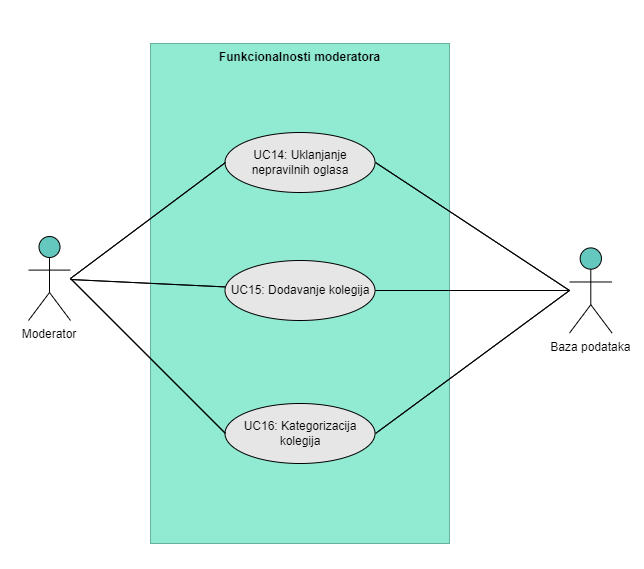
\includegraphics[scale=0.9]{dijagrami/UC_Moderator.PNG}
						\centering
						\caption{Dijagram obrasca uporabe, funkcionalnosti moderatora}
						\label{fig:UC_Moderator}
					\end{figure}
					
			\eject
				
			\subsection{Sekvencijski dijagrami}
			
					\noindent \textbf{Obrazac uporabe UC4 - Registracija}
					
					\noindent Korisnik otvara formu za registraciju i upisuje svoje podatke. Poslužitelj provjerava je li čitava forma popunjena i nalazi li se e-mail u FER-ovoj domeni. Poslužitelj pohranjuje podatke u bazu podataka.  Ukoliko su zauzeti korisničko ime ili e-mail adresa sustav obavještava korisnika o tome i ispisuje poruku.
					
					\begin{figure}[H]
						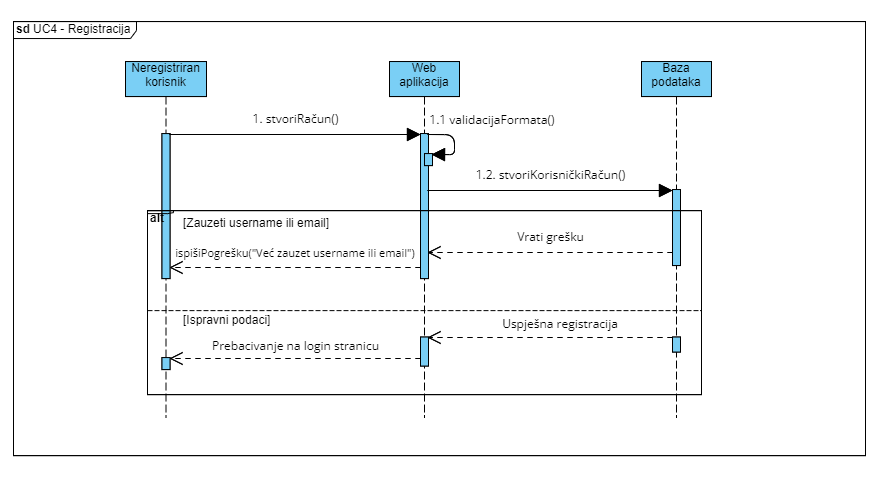
\includegraphics[scale=0.7]{dijagrami/SD_registracija.png}
						\centering
						\caption{Sekvencijski dijagram za UC4}
						\label{fig:SD_registracija}
					\end{figure}
					
			\eject
			
					\noindent \textbf{Obrazac uporabe UC7 - Izmjena objavljenih oglasa}
					
					\noindent Korisnik šalje zahtjev za prikaz aktivnih oglasa. Poslužitelj dohvaća oglase i prikazuje ih korisniku. Korisnik mijenja neke od komponenata oglasa. Poslužitelj provjerava je li koja od komponenata prazna, tj. izbrisana. Ako je promjena validna, ona se pohranjuje u bazu podataka te korisnik dobiva poruku „Promjene unesene“.
					
					\begin{figure}[H]
						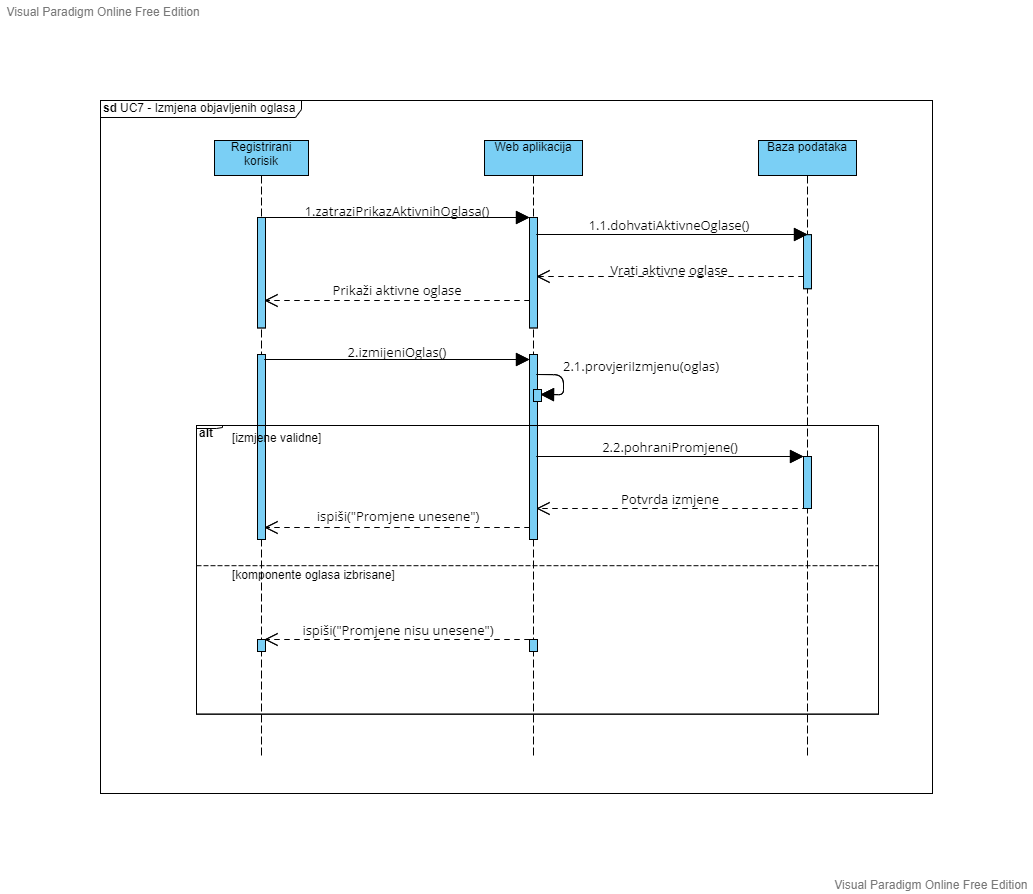
\includegraphics[scale=0.7]{dijagrami/SD_IzmjenaOglasa.png}
						\centering
						\caption{Sekvencijski dijagram za UC7}
						\label{fig:SD_IzmjenaOglasa}
					\end{figure}
					
			\eject
			
					\noindent \textbf{Obrazac uporabe UC13 - Izmjena informacija o profilu}
					
					\noindent Korisnik šalje zahtjev za prikaz aktivnih oglasa. Poslužitelj dohvaća oglase i prikazuje ih korisniku. Korisnik mijenja neke od komponenata oglasa. Poslužitelj provjerava je li koja od komponenata prazna, tj. izbrisana. Ako je promjena validna, ona se pohranjuje u bazu podataka te korisnik dobiva poruku „Promjene unesene“. Ukoliko dođe do greške u obradi zahtjeva sustav obavještava korisnika da promjene nisu unesene.
					
					\begin{figure}[H]
						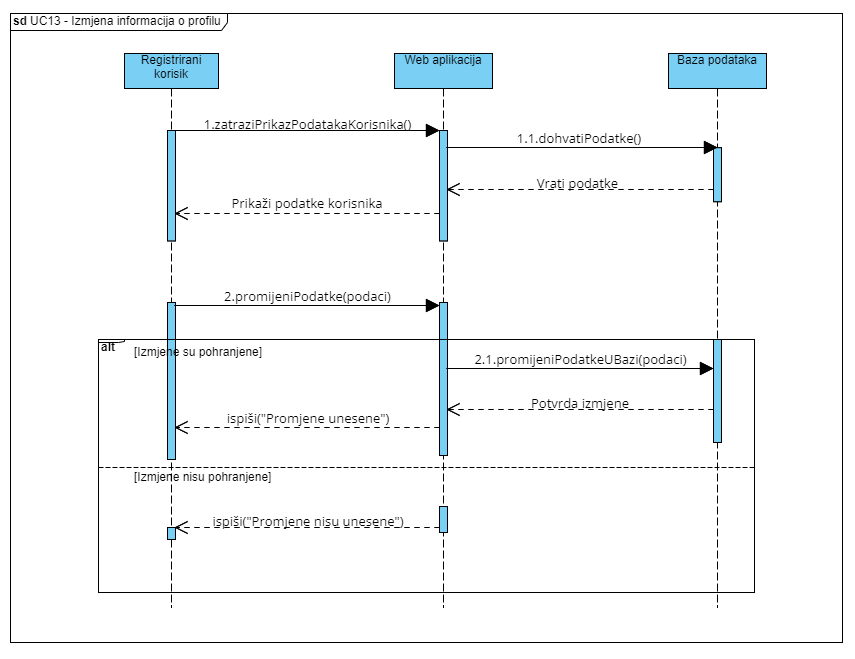
\includegraphics[scale=0.7]{dijagrami/SD_IzmjenaInf.png}
						\centering
						\caption{Sekvencijski dijagram za UC13}
						\label{fig:SD_IzmjenaInf}
					\end{figure}
					
			\eject
			
					\noindent \textbf{Obrazac uporabe UC14 - Uklanjanje nepravilnih oglasa}
					
					\noindent Moderator šalje zahtjev za prikaz aktivnih oglasa. Poslužitelj dohvaća oglase i prikazuje ih korisniku. Ukoliko ne postoje aktivni oglasi, moderator dobiva poruku „Nema aktivnih oglasa za prikaz“. Moderator briše oglas i piše razlog zašto je oglas obrisan. Razlog se šalje korisniku na mail te se oglas briše iz baze podataka. Sustav moderatoru vraća prikaz aktivnih oglasa. Ukoliko su svi oglasi obrisani, moderator dobiva poruku „Nema aktivnih oglasa za prikaz“.
					
					\begin{figure}[H]
						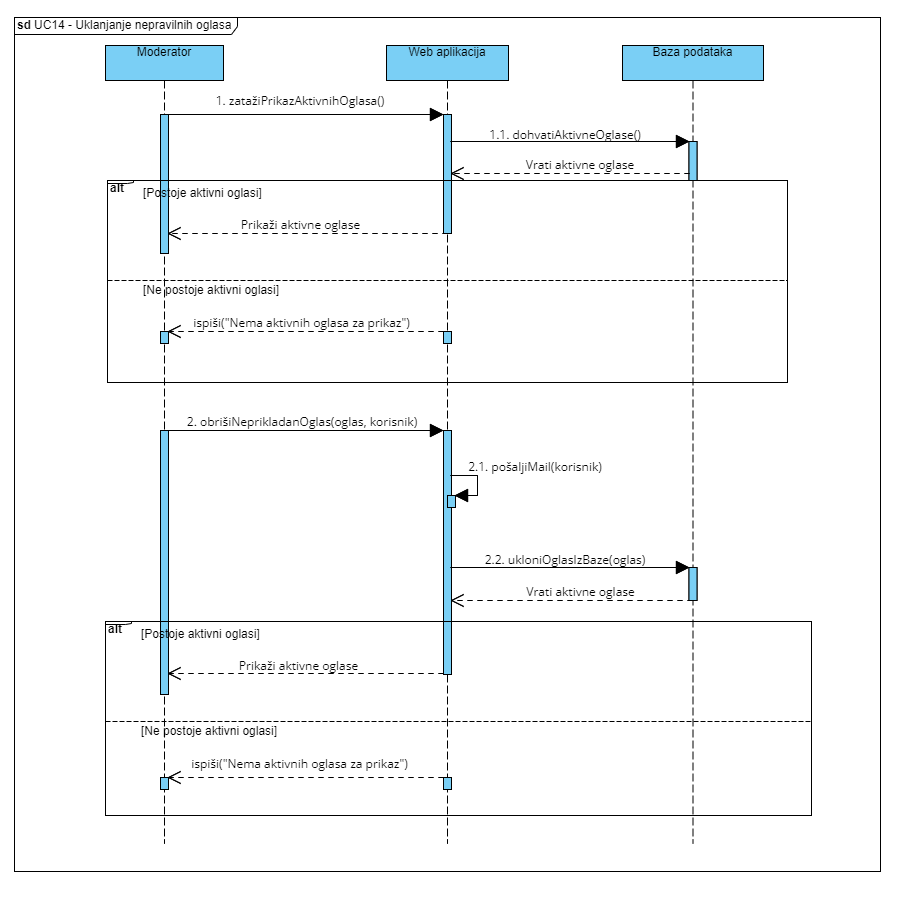
\includegraphics[scale=0.7]{dijagrami/SD_Uklanjanje.png}
						\centering
						\caption{Sekvencijski dijagram za UC14}
						\label{fig:SD_Uklanjanje}
					\end{figure}
	
	\eject
	
	\section{Ostali zahtjevi}
	
		\begin{packed_item}
			
			\item Sustav mora biti napravljena kao web aplikacija koristeći objektno-orijentirane jezike
			\item Aplikacija mora biti prilagodljiva uređajima različitih veličina
			\item Korisničko sučelje mora biti jednostavno za intuitivno korištenje svim korisnicima
			\item Korisničko sučelje i sustav moraju podržavati hrvatsku abecedu pri unosu i prikazu tekstualnog sadržaja
			\item Aplikacija treba omogućiti rad više korisnika u stvarnom vremenu
			\item Neispravno korištenje korisničkog sučelja ne smije narušiti funkcionalnost i rad sustava
			\item Izvršavanje dijela programa u kojem se pristupa bazi podataka ne smije trajati duže od nekoliko sekundi
			\item Slanje e-maila (verifikacijski e-mail ili obrazloženje brisanja oglasa) korisniku ne smije trajati duže od 10 sekundi
			
		\end{packed_item}		
				
			 
			 
			 
	
	\chapter{Arhitektura i dizajn sustava}

		Glavni dijelovi arhitekture sustava su web preglednik, web poslužitelj i baza podataka.  
		
		Web preglednik omogućuje korisniku da pronađe određenu stranicu. Njegova funkcija je prevođenje stranica u svima razumljiv sadržaj. Neki od popularnih web preglednika su Google Chrome, Safari, Microsoft Edge, Opera. 
		
		Web poslužitelj je softverski program koji ima zadatak da pohranjuje, obrađuje i dostavlja klijentima web stranice. Komunikacija između web preglednika i klijenta odvija se HTTPS protokolom. 
		
		Programski jezik koji smo odabrali za implementaciju ove web aplikacije je radni okvir Spring Boot koji koristi višeslojnu arhitekturu. Spring Boot slijedi slojevitu arhitekturu u kojoj svaki sloj komunicira sa slojem neposredno ispod ili iznad njega. Postoje četiri sloja u Spring Boot arhitekturi, a to su: 
		
		\begin{packed_item}
			\item \textbf{Prezentacijski sloj} (engl. \textit{Presentation Layer}) - Ovo je najviši sloj arhitekture. Sastoji se od front-end dijela aplikacije. Obrađuje HTTP zahtjeve, provjerava autentičnost zahtjeva te pretvara JSON parametar u Java objekt. Nakon što provjeri autentičnost zahtjeva, dalje ga prosljeđuje poslovnom sloju.
			\item \textbf{Poslovni sloj} (engl. \textit{Business Layer}) - Ovaj sloj obrađuje svu poslovnu logiku te je zaslužan za autorizaciju i validaciju.
			\item \textbf{Sloj postojanosti} (engl. \textit{Persistence Layer}) - Sadrži svu logiku pohrane te prevodi poslovne objekte iz i u bazu podataka.
			\item \textbf{Sloj baze podataka} (engl. \textit{Database Layer}) - Može se sastojati od više baza podataka. Zaslužan za provođenje CRUD (engl. \textit{Create, Read/Retrieve, Update and Delete}) operacija.
		\end{packed_item}
	
		\begin{figure}[H]
			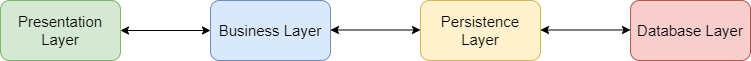
\includegraphics[scale=0.57]{slike/slojevi.png}
			\centering
			\caption{Slojevi Spring Boota}
			\label{fig:slojevi}
		\end{figure}
	
	\eject
	
		Komunikacija u Spring Bootu prikazana je na slici \ref{fig:flow}. Ona započinje kada klijent postavi HTTPS zahtjev koji se dalje šalje nadgledniku. Nadglednik mapira taj zahtjev i obrađuje ga. U sloju usluge obavlja se sva poslovna logika. Spring Boot izvodi svu logiku nad podacima baze podataka koja je preslikana u klasu modela putem Java Persistance biblioteke. U posljetku, ako nije došlo do pogreške, Java Spring Boot stranica se prikazuje klijentu.
				
		\begin{figure}[H]
			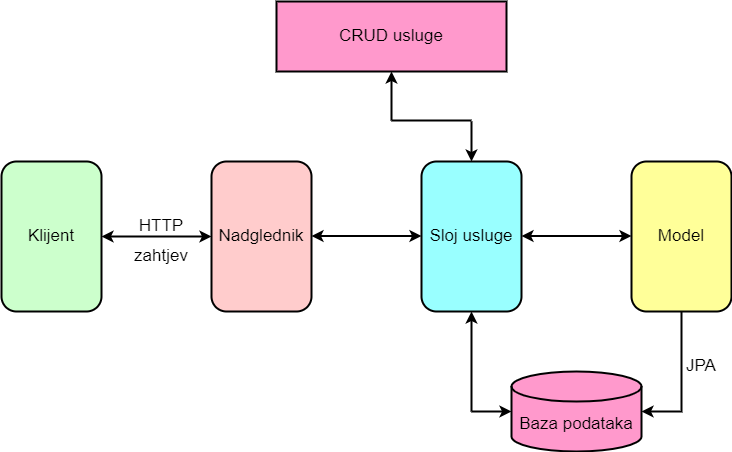
\includegraphics[scale=0.57]{slike/flow.png}
			\centering
			\caption{Komunikacija u Spring Bootu}
			\label{fig:flow}
		\end{figure}
	
		Uz Spring Boot koristili smo React koji je JavaScript biblioteka za izradu korisničkih sučelja. Primarna svrha Reacta je omogućiti razvojnom programeru stvaranje korisničkog sučelja koristeći čisti JavaScript.
		
		Kao razvojne okoline koristili smo IntelliJ IDEA za rad sa Spring Bootom te Visual Studio Code za rad u Reactu. 
		
				
	\eject
	
		\section{Baza podataka}
		
			Za potrebe aplikacije Sinappsa koristit ćemo relacijsku bazu podataka. Osnovna jedinica baze je relacija koja se definira svojim imenom i skupom atributa. Baza podataka pomaže u pohrani, izmjeni i dohvatu podataka koji su nam potrebni za obradu zahtjeva. Baza podataka aplikacije Sinappsa sastoji se od sljedećih entiteta:
			
			\begin{packed_item}
				
				\item Korisnik
				\item Profil
				\item Kolegij
				\item Smjer 
				\item Kategorija
				\item Oglas
				\item Upit
				
			\end{packed_item}
			
			\subsection{Opis tablica}
			
				\noindent \textbf{Korisnik}
				
				\noindent Ovaj entitet sadrži osnovne informacije o korisniku aplikacije. Sadrži jedinstveni identifikator korisnika, njegov email, lozinku i korisničko ime. Osim ovih atributa ova tablica sadrži i boolean zastavicu moderator koja označava je li korisnik moderator sustava ili nije.
				
				\begin{longtblr}[
					label=none,
					entry=none
					]{
						width = \textwidth,
						colspec={|X[10,l]|X[6, l]|X[16, l]|}, 
						rowhead = 1,
					} %definicija širine tablice, širine stupaca, poravnanje i broja redaka naslova tablice
					\hline {\textbf{Korisnik}}	 \\ \hline[3pt]
					\SetCell{LightGreen}id & BIGINT	&  	korisnikov jedinstveni id  	\\ \hline
					email	& VARCHAR &   korisnikov e-mail	\\ \hline 
					lozinka & VARCHAR &  korisnikova lozinka \\ \hline 
					username & VARCHAR	&  	korisnikovo korisničko ime	\\ \hline 
					moderator & BOOLEAN &   oznaka je li korisnik moderator	\\ \hline 
				\end{longtblr}
				
				
				\noindent \textbf{Profil}
				
				\noindent Ovaj entitet sadrži ostale informacije o korisniku i u odnosu je One-To-One sa tablicom Korisnik. Atributi koje ova tablica sadrži su id, ime, prezime, prosječna ocjena, avatar profila, zastavicu potvrđena registracija i strani ključ tablice korisnik idKorisnika.
				
				\begin{longtblr}[
					label=none,
					entry=none
					]{
						width = \textwidth,
						colspec={|X[10,l]|X[6, l]|X[16, l]|}, 
						rowhead = 1,
					} %definicija širine tablice, širine stupaca, poravnanje i broja redaka naslova tablice
					\hline {\textbf{Profil}}	 \\ \hline[3pt]
					\SetCell{LightGreen}id & BIGINT	&  	jedinstvena oznaka profila	\\ \hline
					ime	& VARCHAR &   ime korisnika	\\ \hline 
					prezime & VARCHAR &  prezime korisnika \\ \hline 
					ocjena & VARCHAR	&  	prosječna ocjena studenta-pomagača	\\ \hline 
					potvrđenaRegistracija & BOOLEAN &   oznaka o potvrđenoj registraciji	\\ \hline 
					avatar & VARCHAR &   slika profila	\\ \hline 
					\SetCell{LightBlue}idKorisnika & BIGINT &   referenca na tablicu Korisnik	\\ \hline 
				\end{longtblr}
				
				
				\noindent \textbf{Kolegij}
				
				\noindent Entitet Kolegij sadrži informacije o kolegijima u sustavu. Sadrži atribute: id, naziv kolegija i referencu na tablicu Smjer koja označava na kojem smjeru se predaje kolegij. Relacija Kolegij je u odnosu Many-To-One sa relacijom Smjer.
				
				\begin{longtblr}[
					label=none,
					entry=none
					]{
						width = \textwidth,
						colspec={|X[10,l]|X[6, l]|X[16, l]|}, 
						rowhead = 1,
					} %definicija širine tablice, širine stupaca, poravnanje i broja redaka naslova tablice
					\hline {\textbf{Kolegij}}	 \\ \hline[3pt]
					\SetCell{LightGreen}id & BIGINT	&  	jedinstvena oznaka kolegija	\\ \hline
					nazivKolegija	& VARCHAR &   naziv kolegija	\\ \hline  
					\SetCell{LightBlue}idSmjera & BIGINT &   referenca na relaciju Smjer	\\ \hline 
				\end{longtblr}
				
				\noindent \textbf{Smjer}
				
				\noindent Entitet Smjer sadrži dva atributa, id i nazivSmjera. Ova tablica pohranjuje smjerove koji se predaju na FER-u kako bi se kolegiji mogli svrstati po tim smjerovima.
				
				\begin{longtblr}[
					label=none,
					entry=none
					]{
						width = \textwidth,
						colspec={|X[10,l]|X[6, l]|X[16, l]|}, 
						rowhead = 1,
					} %definicija širine tablice, širine stupaca, poravnanje i broja redaka naslova tablice
					\hline {\textbf{Smjer}}	 \\ \hline[3pt]
					\SetCell{LightGreen}id & BIGINT	&  	jedinstvena oznaka smjera	\\ \hline
					nazivSmjera	& VARCHAR &   naziv smjera	\\ \hline  
				\end{longtblr}
				
				\noindent \textbf{Kategorija}
				
				\noindent Entitet Kategorija pohranjuje informacije o različitim kategorijama za koje se može napraviti oglas. Atributi u ovoj tablici su id i nazivKategorije. Mogući nazivi kategorija su: laboratorijska vježba, blic, gradivo, kontinuirani ispit, ispitni rok.
				
				\begin{longtblr}[
					label=none,
					entry=none
					]{
						width = \textwidth,
						colspec={|X[10,l]|X[6, l]|X[16, l]|}, 
						rowhead = 1,
					} %definicija širine tablice, širine stupaca, poravnanje i broja redaka naslova tablice
					\hline {\textbf{Kategorija}}	 \\ \hline[3pt]
					\SetCell{LightGreen}id & BIGINT	&  	jedinstvena oznaka kategorije	\\ \hline
					nazivKategorije	& VARCHAR &   naziv kategorije	\\ \hline  
				\end{longtblr}
				
				\noindent \textbf{Oglas}
				
				\noindent Ovaj entitet predstavlja oglas koji student-pomagač objavljuje u aplikaciji. Sadrži atribute id, naslov, opis i reference na relacije Kategorija, Kolegiji i Profil. Pomoću reference na relaciju Kategorija oglasu se određuje u koju kategoriju oglasa spada: laboratorijska vježba, blic, gradivo, kontinuirani ispit, ispitni rok. Određeni oglas objavljen je za određeni kolegij te se ta informacija pamti pomoću reference na relaciju Kolegij. Također pomoću reference na relaciju profil pamti se informacija koji student-pomagač je objavio oglas. Sa entitetima Kategorija, Kolegij, Profil ovaj entitet ima odnos One-To-One.
				
				\begin{longtblr}[
					label=none,
					entry=none
					]{
						width = \textwidth,
						colspec={|X[10,l]|X[6, l]|X[16, l]|}, 
						rowhead = 1,
					} %definicija širine tablice, širine stupaca, poravnanje i broja redaka naslova tablice
					\hline {\textbf{Oglas}}	 \\ \hline[3pt]
					\SetCell{LightGreen}id & BIGINT	&  	jedinstvena oznaka oglasa	\\ \hline
					naslov	& VARCHAR &   naslov oglasa	\\ \hline 
					opis & VARCHAR &  opis oglasa \\ \hline 
					\SetCell{LightBlue}idKategorije & BIGINT	&  	referenca na relaciju Kategorija	\\ \hline 
					\SetCell{LightBlue}idKolegija & BIGINT &   referenca na relaciju Kolegij	\\ \hline 
					\SetCell{LightBlue}idPomagača & BIGINT &   referenca na relaciju Profil	\\ \hline 
				\end{longtblr}
			
			\eject
				
				\noindent \textbf{Upit}
				
				\noindent Entitet upit predstavlja sve upite koje studenti pošalju na jedan oglas. Sadrži sljedeće atribute: id, poruka, statusUpita i reference na relacije Oglas i Profil. Atribut id je jedinstveni identifikator upita. Atribut poruka sadrži poruku koju student koji se javlja na oglas šalje studentu-pomagaču koji je objavio oglas. Atribut statusUpita može imati jednu od 3 vrijednosti: 0 – U tijeku (upit čeka odgovor studenta pomagača),  1 – Odbijen (student-pomagač je odbio upit) i 2 – Prihvaćen (student-pomagač je odobrio upit). Pomoću reference na relaciju Oglas baza pamti za koji oglas student šalje upit, a pomoću reference na relaciju Profil pamti se koji student šalje upit. S obje relacije veza je One-To-One.
				
				\begin{longtblr}[
					label=none,
					entry=none
					]{
						width = \textwidth,
						colspec={|X[10,l]|X[6, l]|X[16, l]|}, 
						rowhead = 1,
					} %definicija širine tablice, širine stupaca, poravnanje i broja redaka naslova tablice
					\hline {\textbf{Upit}}	 \\ \hline[3pt]
					\SetCell{LightGreen}id & BIGINT	&  	jedinstvena oznaka upita	\\ \hline
					poruka	& VARCHAR &   poruka koju šalje pošiljatelj	\\ \hline 
					statusUpita & INTEGER &  status upita \\ \hline 
					\SetCell{LightBlue}idOglas & BIGINT	&  	referenca na relaciju Oglas	\\ \hline 
					\SetCell{LightBlue}idPošiljatelja & BIGINT &   referenca na relaciju Profil	\\ \hline 
				\end{longtblr}
			
			\eject
				
			\subsection{Dijagram baze podataka}
				
				\begin{figure}[H]
					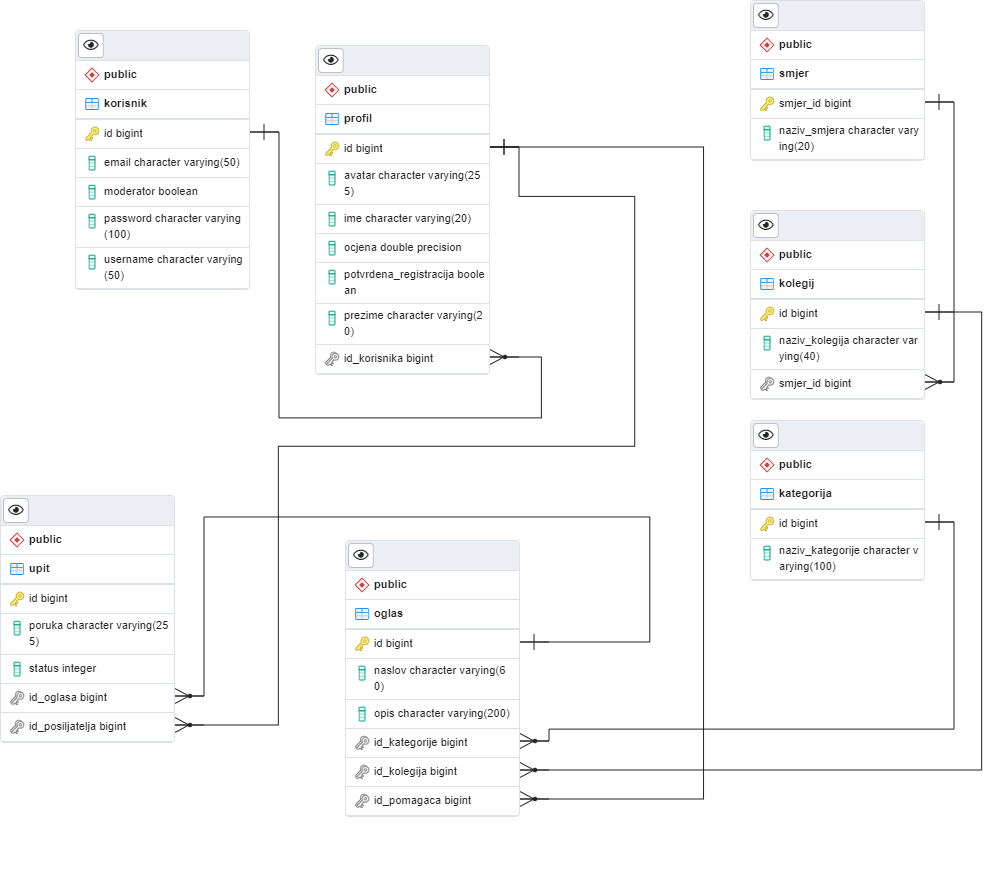
\includegraphics[scale=0.6]{dijagrami/baza.png}
					\centering
					\caption{Dijagram baze podataka}
					\label{fig:dijagram baze}
				\end{figure}
				
			\eject
			
			
		\section{Dijagram razreda}
		
			Na slikama \ref{fig:cont}, \ref{fig:DAO} i \ref{fig:models} prikazani su razredi koji pripadaju backend dijelu MVC arhitekture. Razredi su podijeljeni u tri dijela: Controllers, DAO i Modele. Razredi u Controllers dijelu nasljeđuju razred Controller i upravljaju pristiglim zahtjevima na backend dio aplikacije. Metode implementirane u tim razredima manipuliraju s DAO (Dana Access Object) razredima. DAO razredi su modelirani i dohvaćeni pomoću metoda koje su implentirane u Model razredima. Povratne vrijednosti metoda u Controller razredima su JSON datoteke s HTML status kodom.
			
			Zbog lakšeg prikaza i organizacije, razredi su logički podijeljeni po pravu pristupa metodama određenih aktora te su prikazane samo ovisnosti između razreda koji pripadaju istom dijelu dijagrama. Iz naziva i tipova atributa u razredima može se zaključiti vrsta ovisnosti među različitim razredima.
			
			\begin{figure}[H]
				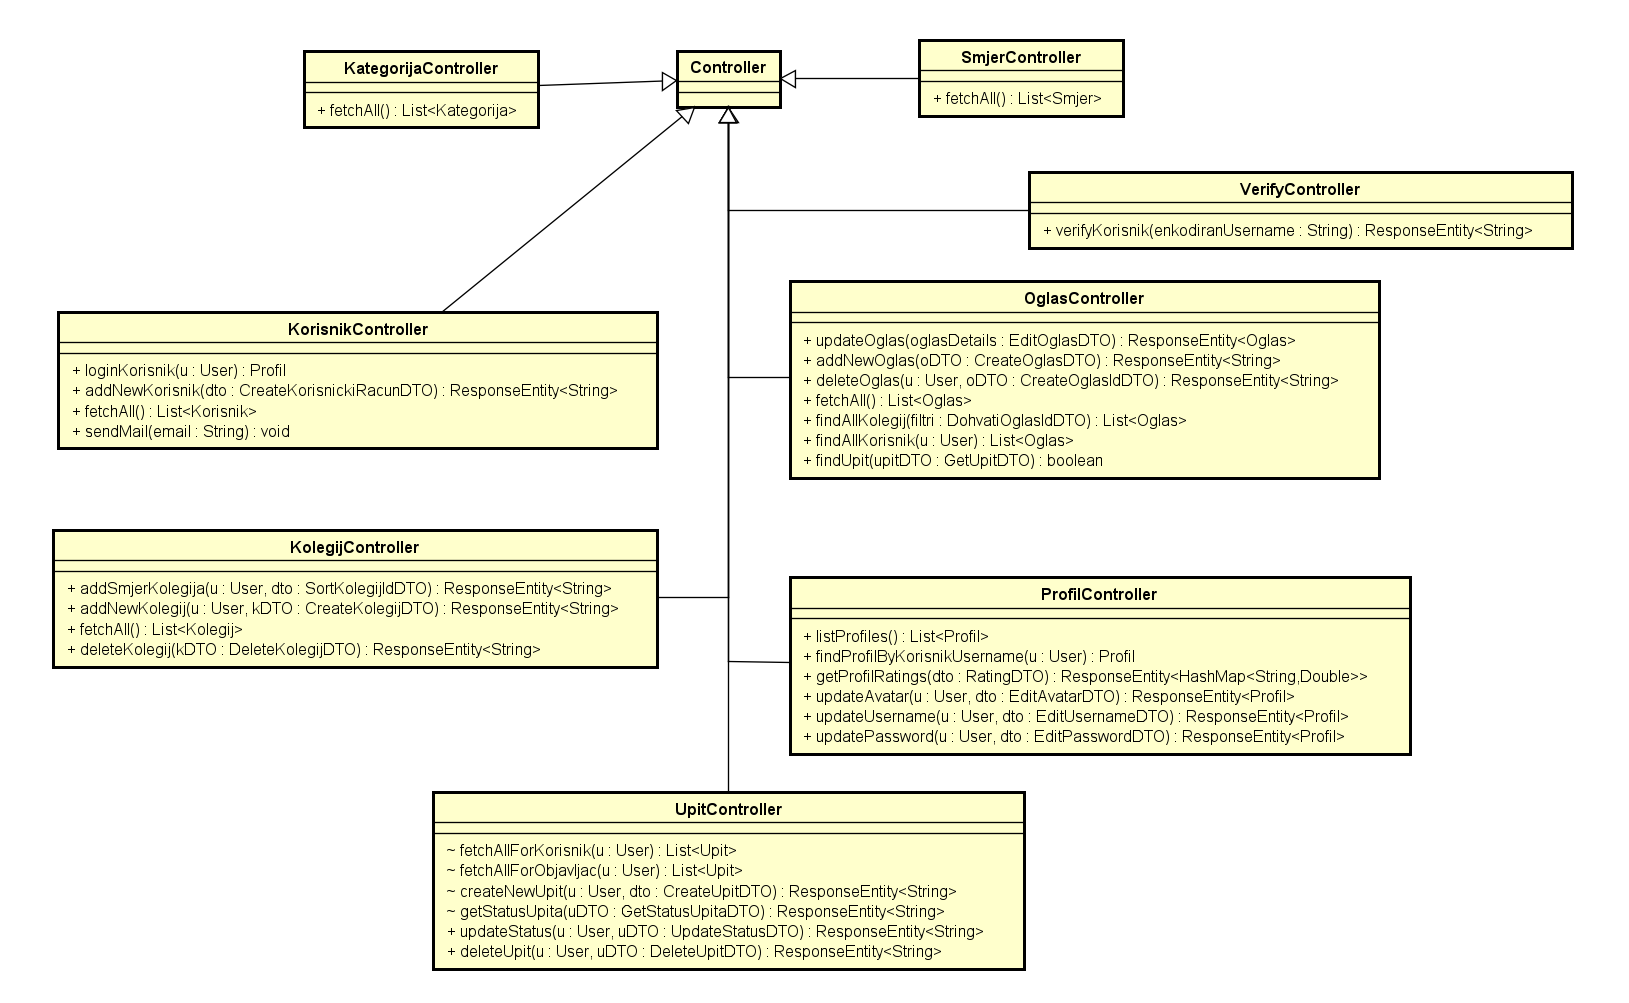
\includegraphics[scale=0.35]{dijagrami/dijagram_razreda_controllers.png}
				\centering
				\caption{Dijagram razreda - Controllers}
				\label{fig:cont}
			\end{figure}
		
			\begin{figure}[H]
				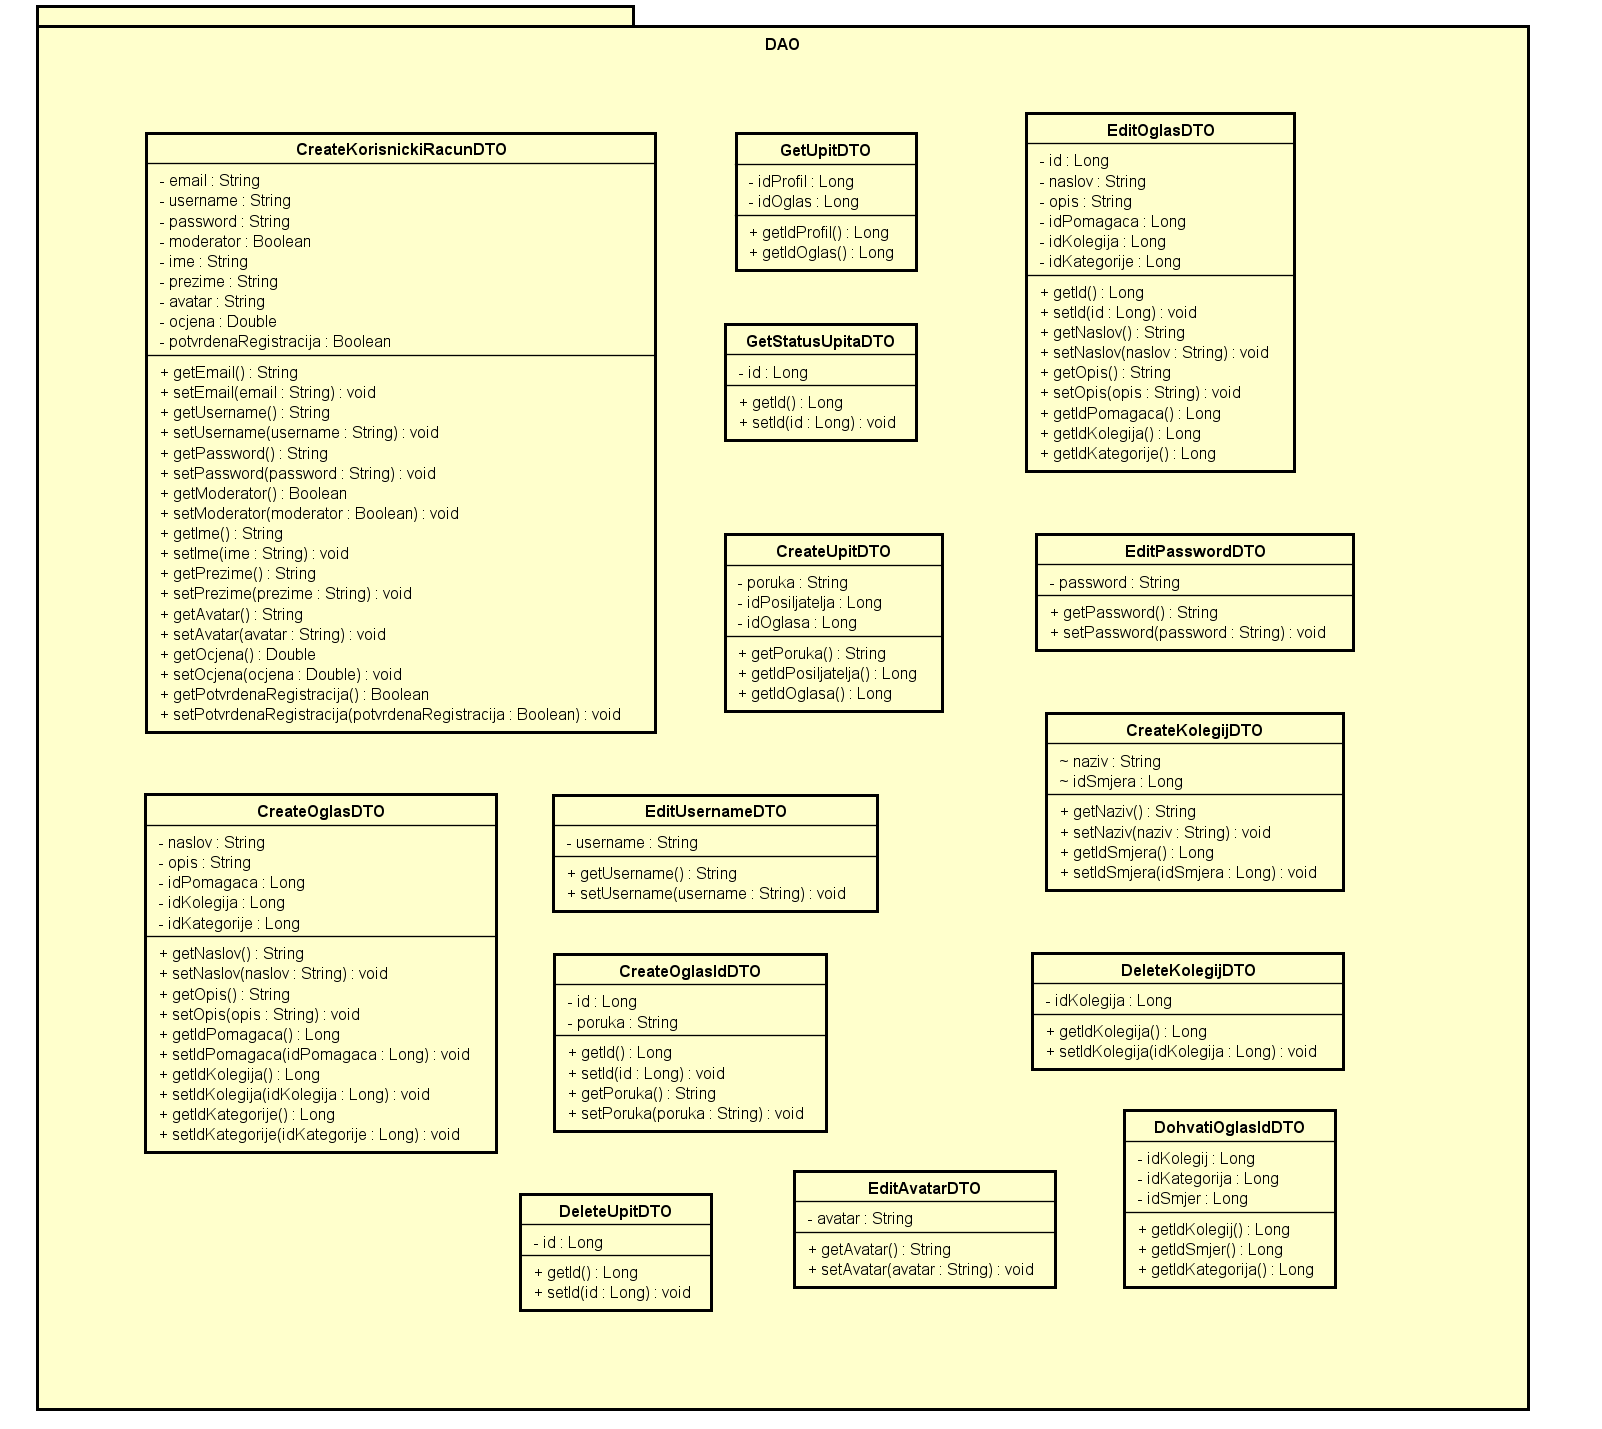
\includegraphics[scale=0.37]{dijagrami/dijagram_razreda_DAO.png}
				\centering
				\caption{Dijagram razreda - Dana Access Object}
				\label{fig:DAO}
			\end{figure}
			
			Razredi modela preslikavaju strukturu baze podataka u aplikaciju. Implementirane metode komuniciraju s bazom te vraćaju tražene podatke. Razred Korisnik predstavlja registriranog korisnika i njegovo osnovne informacije važne za prijavu i slanje e-maila: e-mail adresa, korisničko ime i zaporka. Razred Profil sadrži više dodatnih informacija o registriranom korisniku kao što su ime, prezime, odabrani avatar i status je li registracija potvrđena putem maila ili nije. Razred Smjer predstavlja dostupne smjerove na studiju. Razred Kolegij sadrži informacije o kolegijima koji su dodani u bazu. Dostupne informacije su naziv kolegija i smjer kojem taj kolegij pripada. Razred Kategorija predstavlja kategoriju u koju možemo svrstati oglas. U sustavu postoji 5 različitih kategorija: laboratorijska vježba, blic, gradivo, kontinuirani ispit i ispitni rok. Razred Oglas predstavlja informacije koje se pohranjuju u bazu za pojedini oglas, a to su: naziv oglasa, opis oglasa, kolegij za koji se oglas objavljuje, kategorija kojoj oglas pripada i profil koji je poslao upit za taj oglas. Razred Upit pamti podatke vezane uz javljanje na određeni oglas. Sadrži oglas za koji se šalje upit, sadrži profil koji stvara upit, poruku s kojom korisnik šalje upit i status u kojem se nalazi upit. Razred StatusUpita predstavlja enumeraciju pomoću koje se modelira jedan od 3 stanja upita: u tijeku, prihvaćen i odbijen.
			
			\begin{figure}[H]
				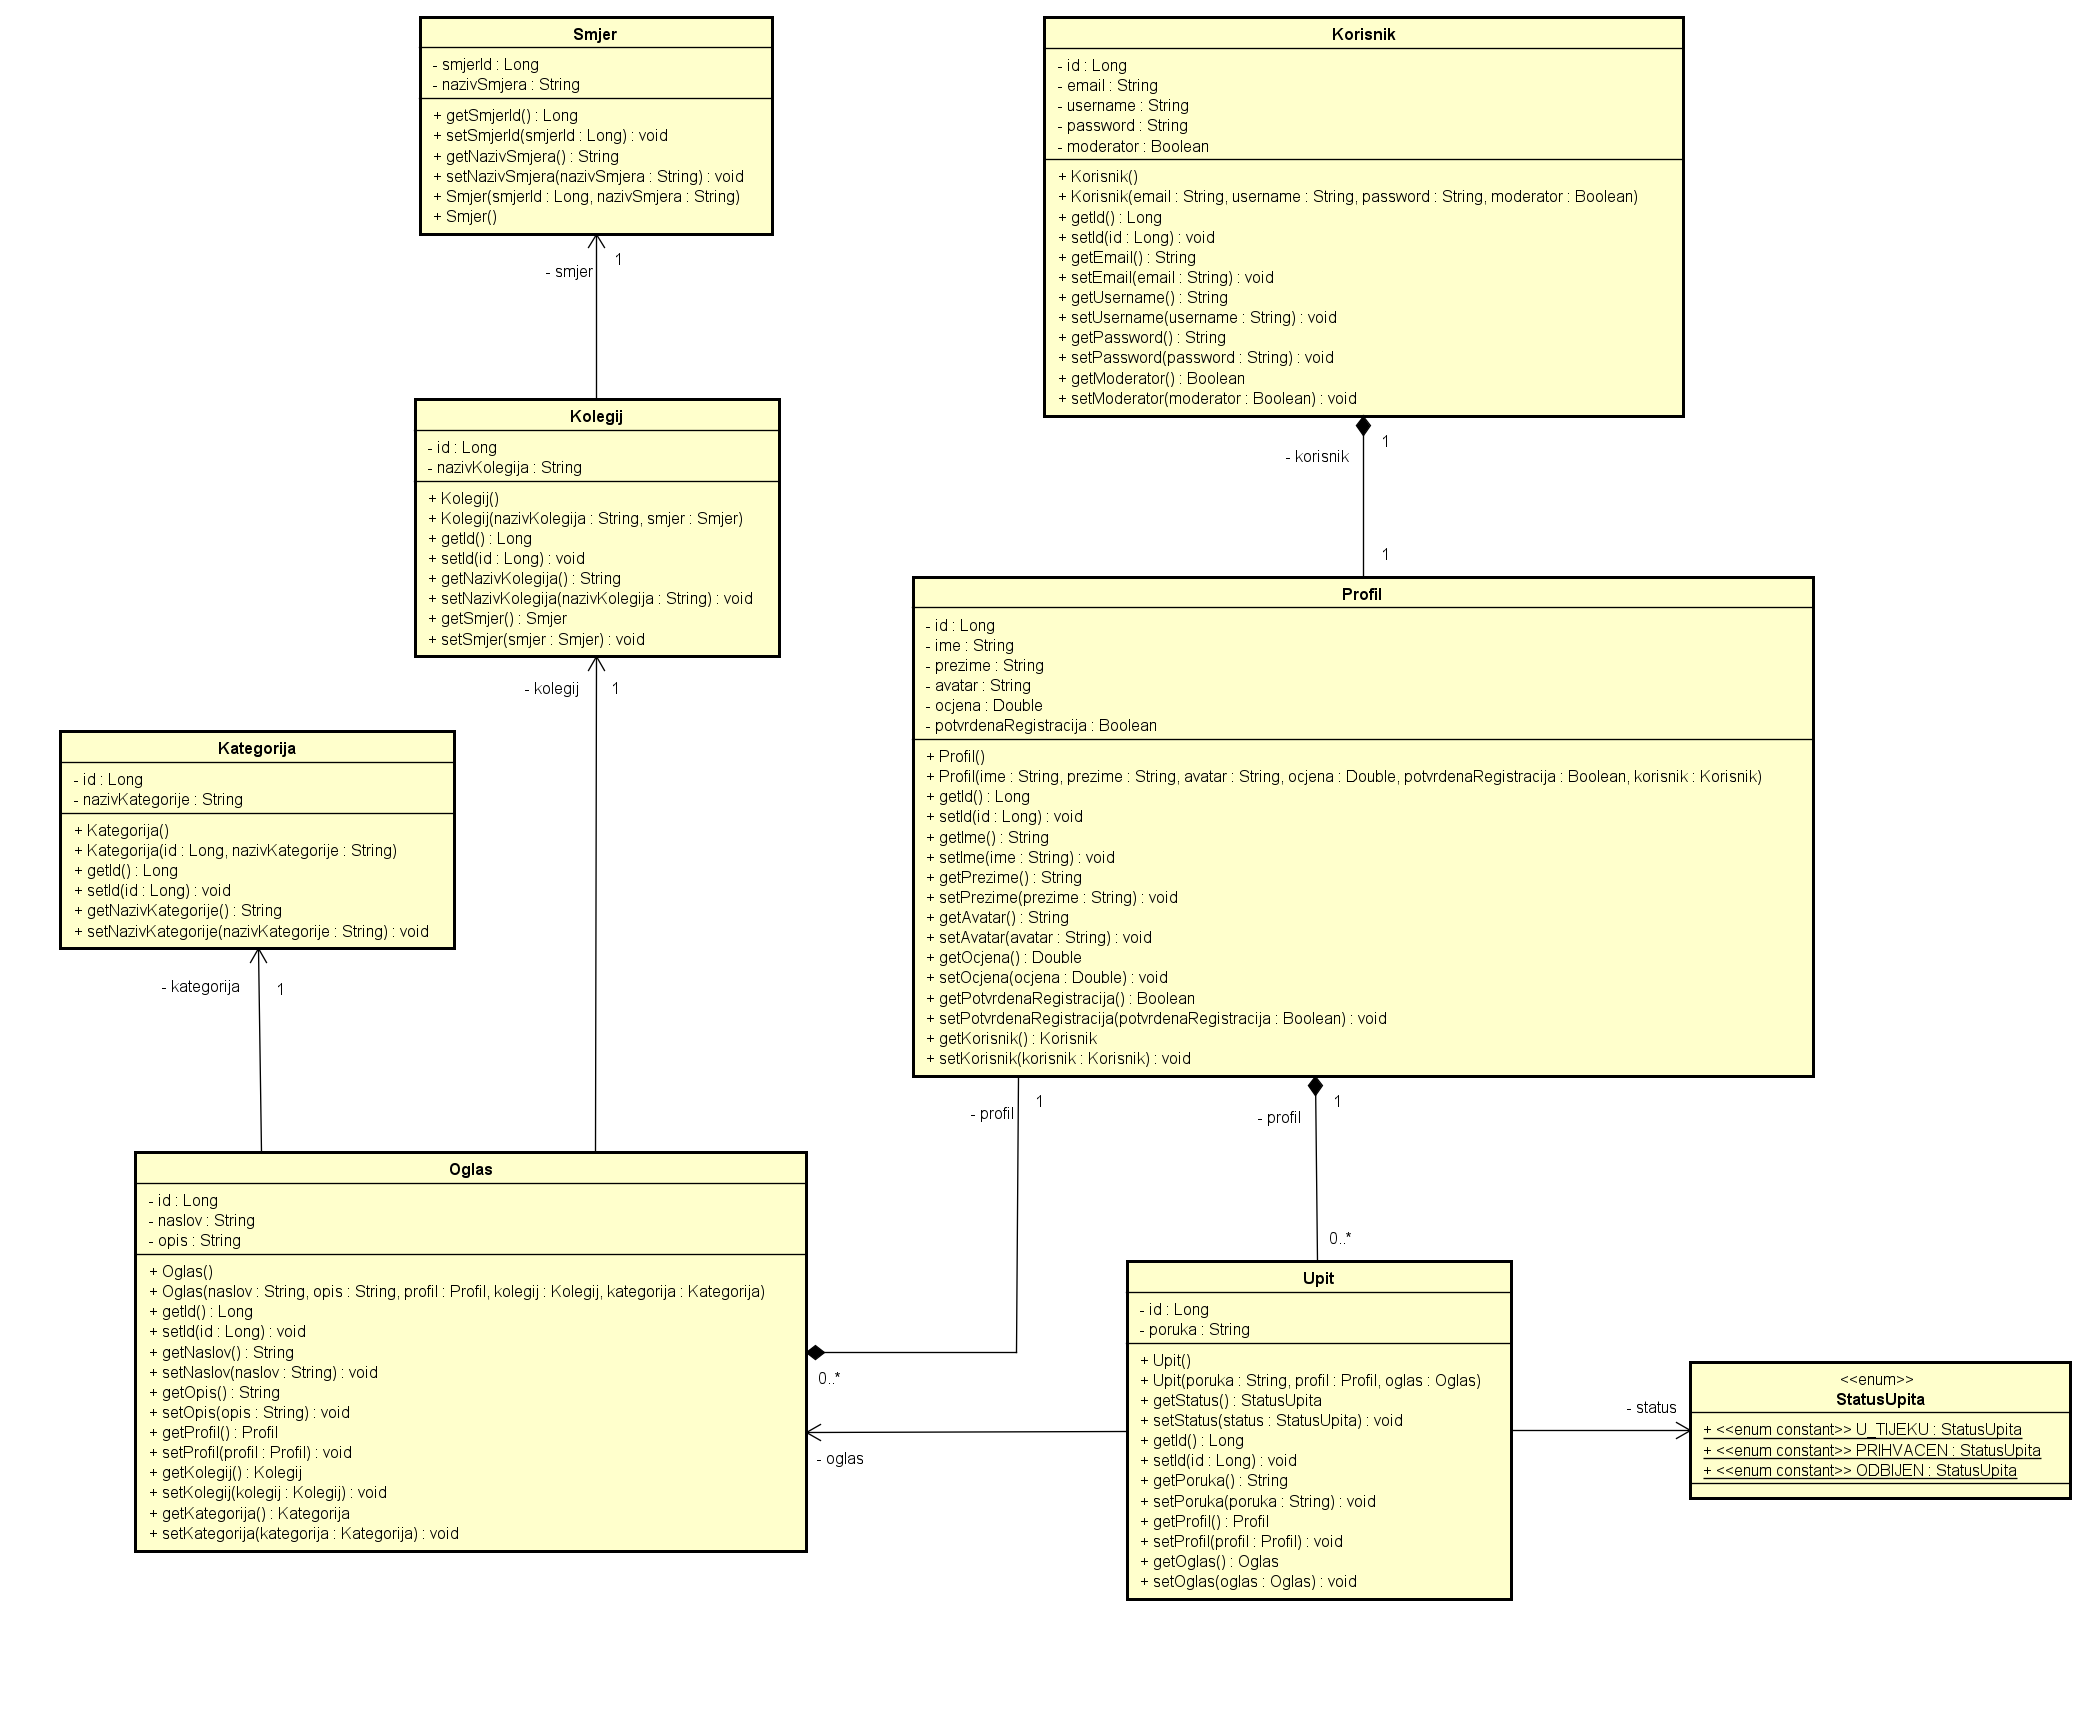
\includegraphics[scale=0.28]{dijagrami/dijagram_razreda_models.png}
				\centering
				\caption{Dijagram razreda - Models}
				\label{fig:models}
			\end{figure}
		
			\eject
		\section{Dijagram stanja}
			Na slici \ref{fig:dijagram stanja} prikazan je dijagram stanja. On prikazuje dinamičko ponašanje dijela sustava. Dijagram opisuje stanja za registriranog korisnika. Korisnik nakon prijave dolazi na početnu stranicu. Tamo ima mogućnost stvaranja novog oglasa, javljanja na tuđe oglase, filtriranja po smjeru, kolegiju i kategoriji te odlazak na stanicu „Profile“. Na stranici profila korisnik ima mogućnost uređivanja svojih podataka, tj. mijenjanja avatara, lozinke i nadimka. Ako postoji upit na oglas koje je napisao korisnik, onda korisnik ima mogućnost prihvatiti ili odbiti taj upit. U dijelu „Moji objavljeni oglasi“ korisnik ima mogućnost uređivanja oglasa, klikom na ikonu olovke, ili brisanja oglasa, klikom na ikonu smeća. Korisnik iz svih stanja može doći u stanje početne stranice i stranice profila te se iz svih stanja može odjaviti.
		
			\begin{figure}[H]
				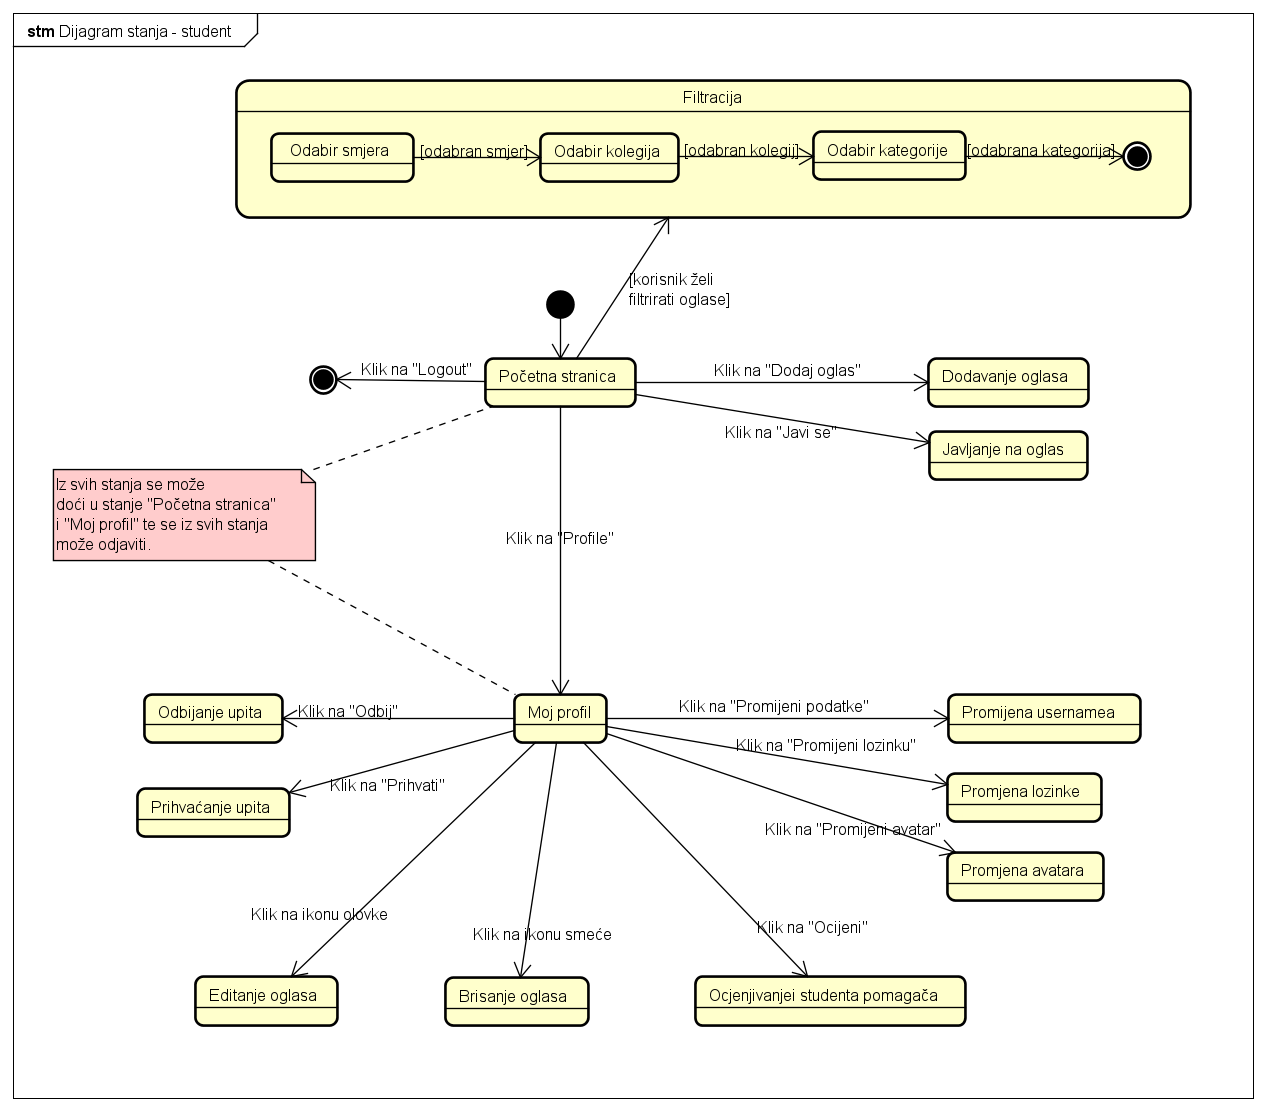
\includegraphics[scale=0.45]{dijagrami/DijagramStanja.png}
				\centering
				\caption{Dijagram stanja}
				\label{fig:dijagram stanja}
			\end{figure}
			
			\eject 
		
		\section{Dijagram aktivnosti}
			Dijagram aktivnosti koristi se za modeliranje poslovnih procesa ili upravljačkog i podatkovnog toka. Na slici \ref{fig:dijagram aktivnosti} prikazan je dijagram aktivnosti registriranog korisnika. Korisnik nakon prijave stvara novi oglas nakon čega preko e-maila dobiva upit na stvoreni oglas. Korisnik odabire hoće li prihvatiti ili obiti upit na oglas. Zatim se korisnik javlja na oglas nekog drugog studenta pomagača te nakon potvrđenog upita na oglas ocjenjuje instrukcije. Na posljetku korisnik briše svoj oglas te se odjavljuje.
			
			\begin{figure}[H]
				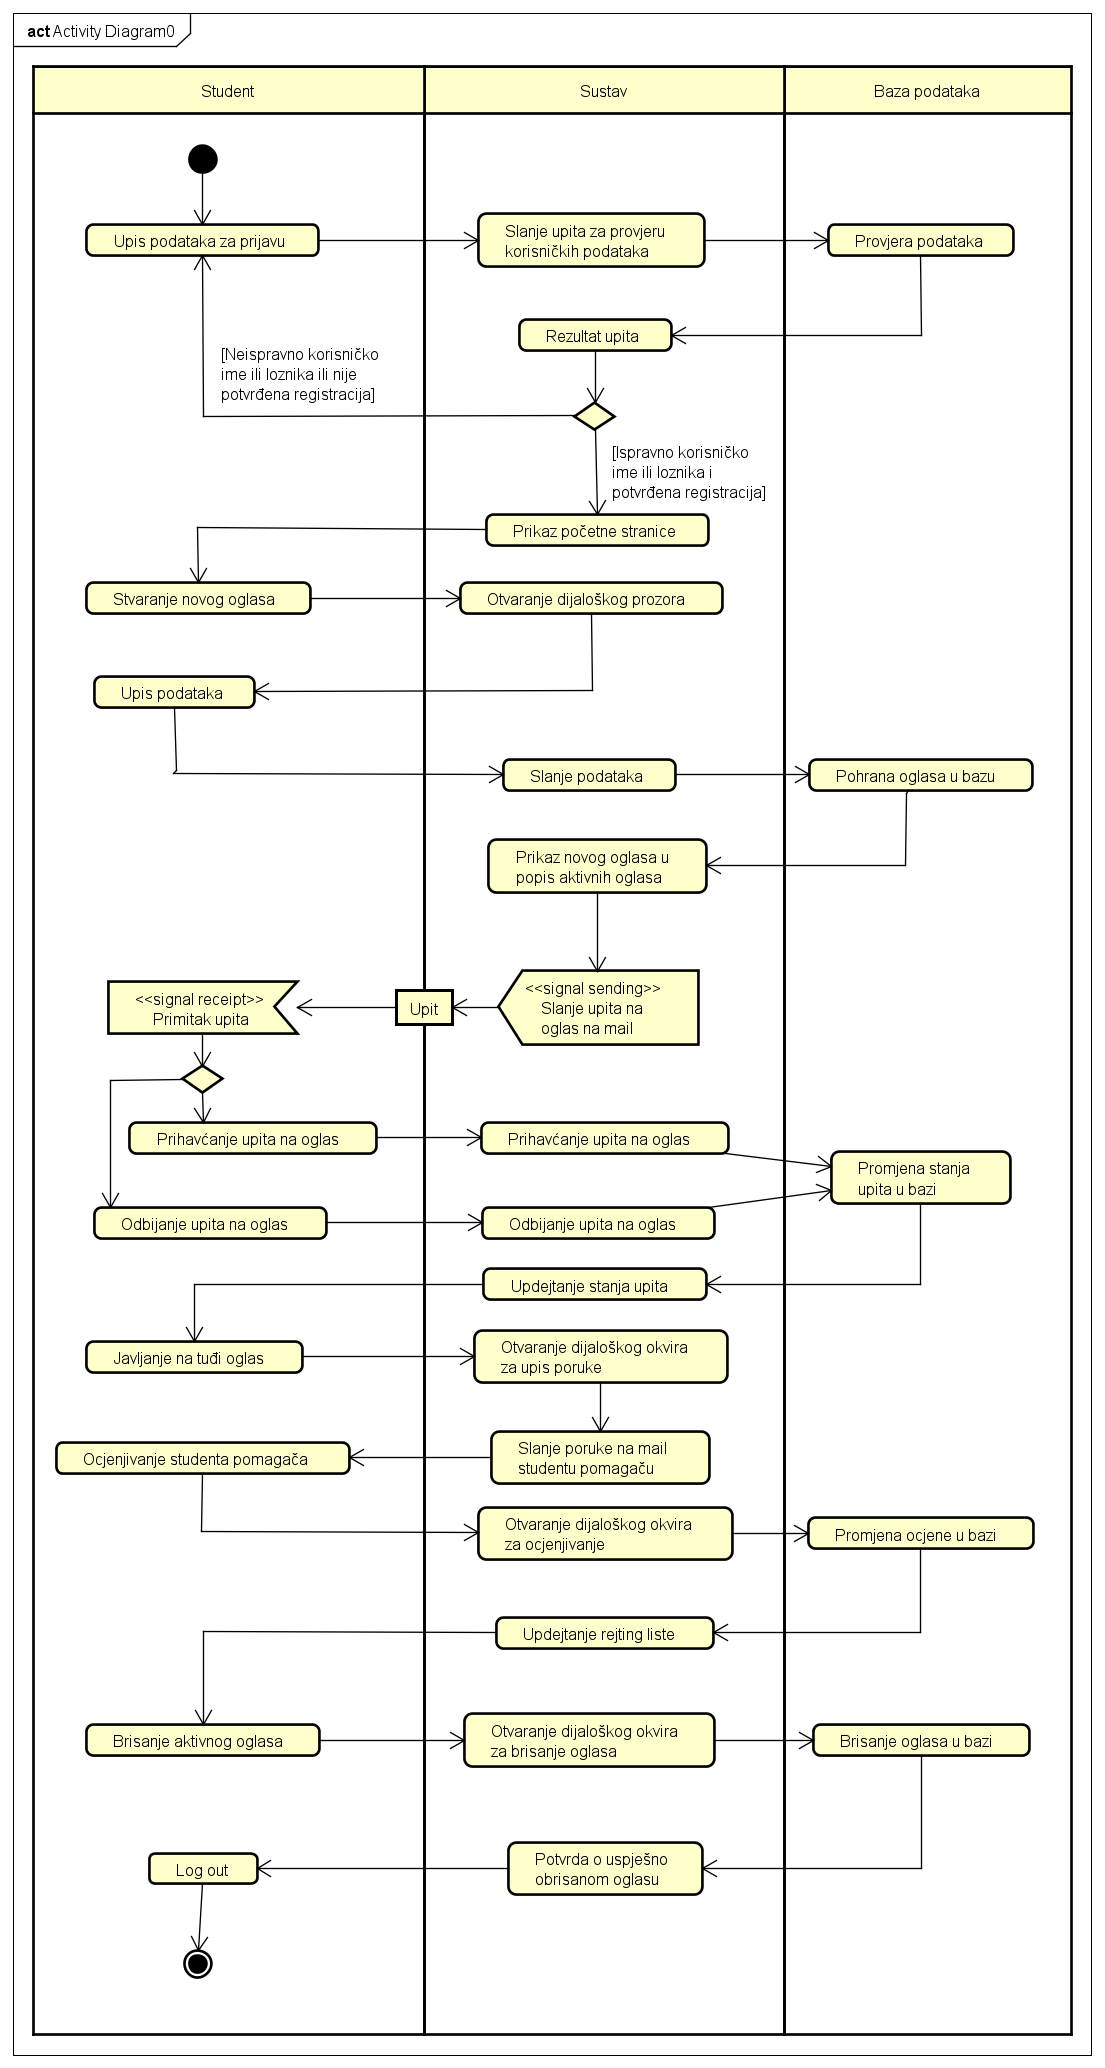
\includegraphics[scale=0.42]{dijagrami/DijagramAktivnosti.png}
				\centering
				\caption{Dijagram aktivnosti}
				\label{fig:dijagram aktivnosti}
			\end{figure}
			
			\eject
			
		\section{Dijagram komponenti}
		Dijagram komponenti prikazan na slici \ref{fig:dijagram konponenti} opisuje međusobnu ovisnost komponenti, internu strukturu komponenti i njihov odnos prema okolini. Sustavu se pristupa preko dva sučelja. Prvo sučelje služi za dohvat HTML, CSS i JS datoteka. To sučelje pripada frontend dijelu aplikacije. Router je komponenta koja na temelju url određuje koje datoteke će sučelje vratiti kao rezultat upita. Frontend dio aplikacije sastoji se od niza JavaScript datoteka koje su raspoređene u logičke cjeline. Te logičke cjeline nazvane su po različitim tipovima aktora koji pristupaju aplikaciji. Sve JavaScript datoteke u logičkim cjelinama ovise o React biblioteci pomoću koje se dohvaćaju gotove komponente kao što su polja za upis podataka, gumbi, odlomci, itd. Drugo sučelje pomoću kojeg se može pristupiti aplikaciji je sučelje koje služi za dohvat JSON podataka. Preko tog sučelja pristupa se REST API komponenti sustava. REST API poslužuje podatke koji pripadaju backend dijelu aplikacije. Hibernate je implementacija JPA putem kojeg se pomoću SQL upita može pristupiti i dohvatiti podatke iz baze podataka. Tako dohvaćeni podaci iz baze šalju se dalje MVC arhitekturi u obliku DAO (Data Access Object). React-view je komponenta koja preko dostupnih sučelja komunicira sa Sinappsa aplikacijom te ovisno o korisnikovim akcijama osvježava prikaz i dohvaća nove podatke od aplikacije.  
		
		\begin{figure}[H]
			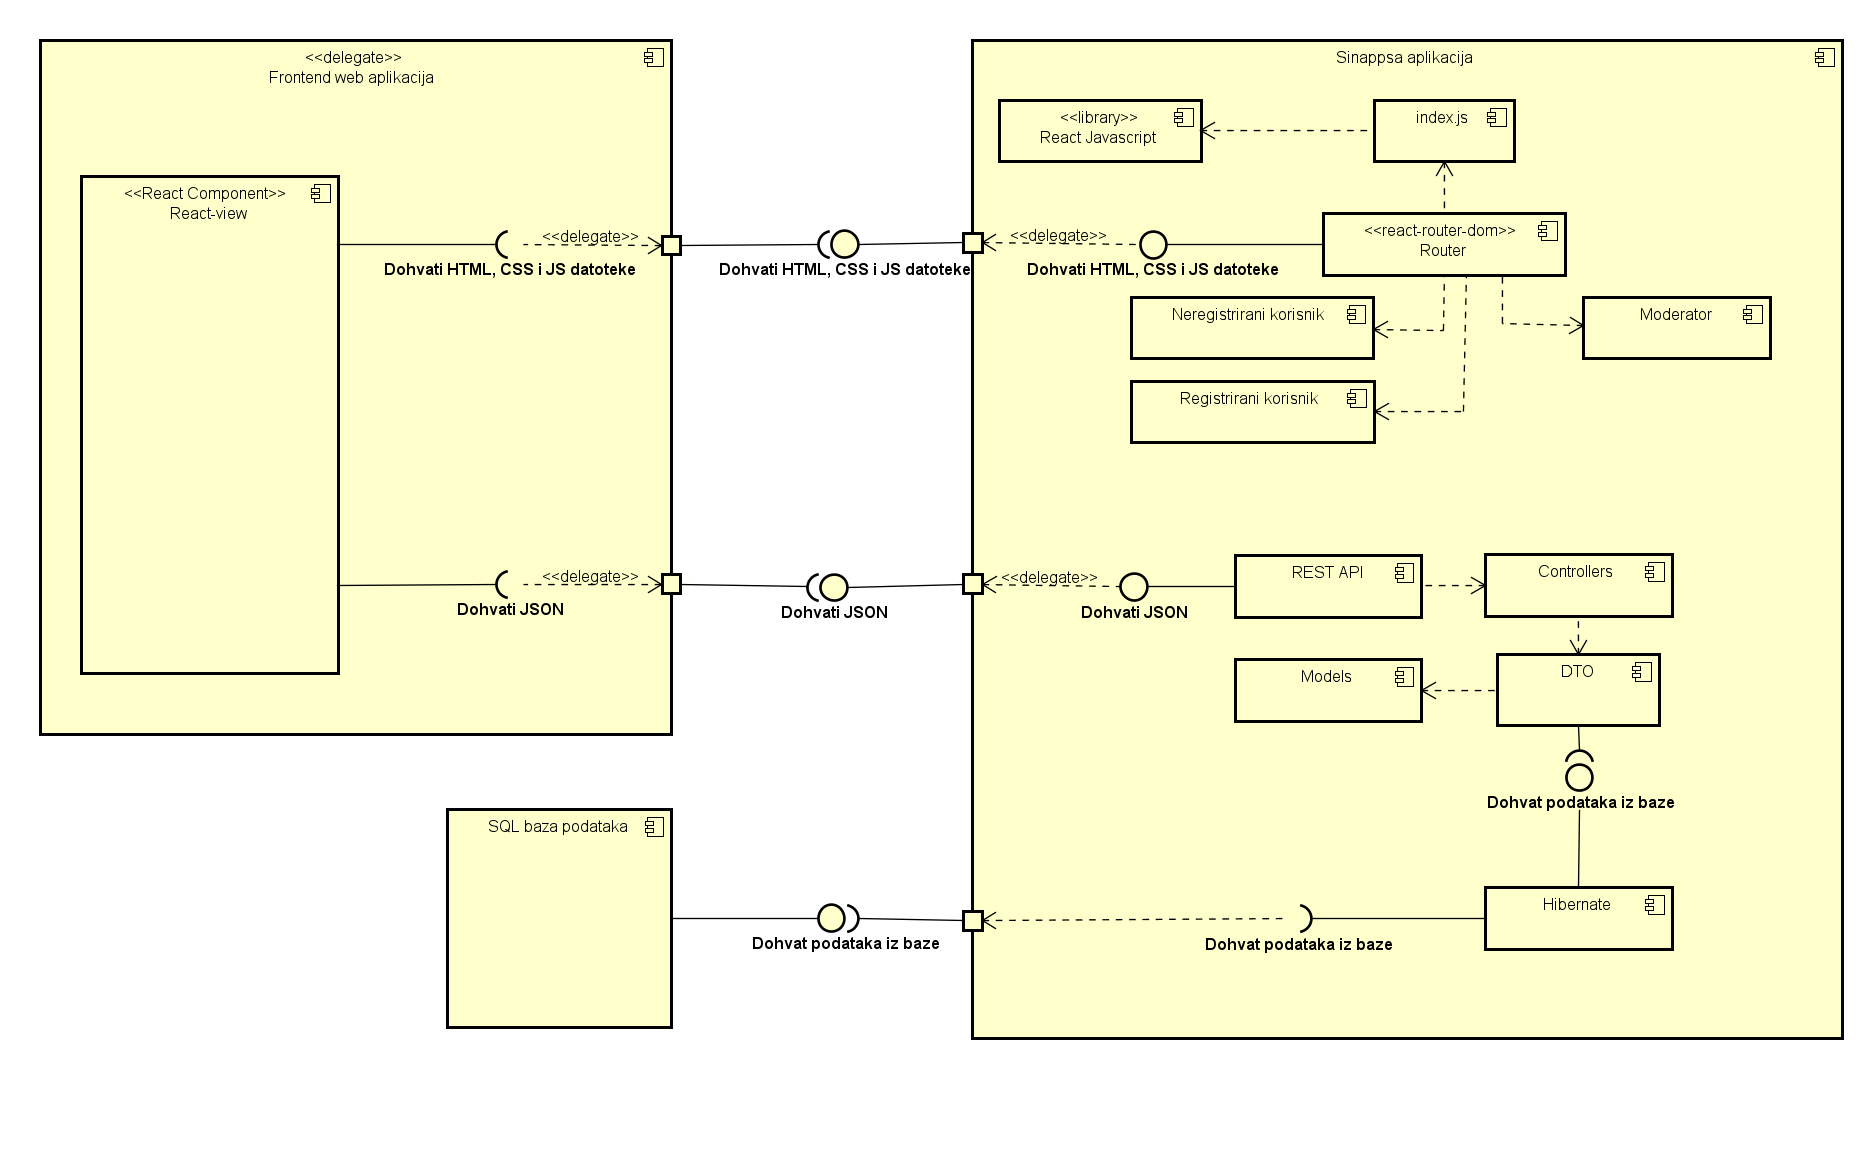
\includegraphics[scale=0.31]{dijagrami/dijagram_komponenti.png}
			\centering
			\caption{Dijagram komponenti}
			\label{fig:dijagram konponenti}
		\end{figure}
		
	\chapter{Implementacija i korisničko sučelje}
		
		
		\section{Korištene tehnologije i alati}
			Za komunikaciju između članova tima korištene su aplikacije WhatsApp\footnote{https://www.whatsapp.com/} i Microsoft Teams\footnote{https://www.microsoft.com/en-us/microsoft-teams/group-chat-software}. Upravljanje programskim kodom se obavljalo preko distribuiranog sustava Git\footnote{https://git-scm.com/} te je korišten udaljeni repozitorij GitLab\footnote{https://about.gitlab.com/}.
			
			Za izradu korisničkih sučelja, tj. frontenda, korištena je JavaScript biblioteka React ili React.js\footnote{https://reactjs.org/} koja se koristi za brzu i učinkovitu izgradnju interaktivnih korisničkih sučelja i web aplikacija uz znatno manje napisanog koda. U Reactu aplikacije se razvijaju stvaranjem komponenti za višestruku uporabu. React je izgrađen pomoću JSX-a – kombinacije JavaScripta i XML-a. Razvio ga je Facebook. Razvojna okolina korištena za rad u Reactu je Visual Studio Code\footnote{https://code.visualstudio.com/}. VS Code besplatno je Microsoftovo razvojno okruženje otvorenog koda (engl. open source). Danas jedan od najpopularnijih uređivača izvornog koda koji omogućuje programiranje u velikom izboru programskih jezika. 
			
			Implementacija ove web aplikacije, tj. backend, napravljena s radnim okvirom Spring Boot\footnote{https://spring.io/projects/spring-boot}. Spring Boot je mikro framework otvorenog koda koji održava tvrtka Pivotal. Koristi Javu te je zgrađen na temelju Spring okvira. On pruža lakši i brži način za postavljanje, konfiguriranje i pokretanje aplikacija. Za pisanje backenda korišteno je razvojno okruženje InteliJ IDEA\footnote{https://www.jetbrains.com/idea/}. To je integrirano razvojno okruženje (IDE) napisano u Javi za razvoj računalnog softvera napisanog u Javi, Kotlinu , Groovyju i drugim jezicima koji se temelje na JVM -u. Razvio ga je JetBrains. Pruža određene značajke kao što je dovršavanje koda analizom konteksta, navigacija koda koja omogućuje izravno skakanje u klasu ili deklaraciju u kodu, refaktoriranje koda , otklanjanje pogrešaka koda i opcije za ispravljanje nedosljednosti putem prijedloga.
			
			Za pisanje dokumentacije korišten je markup jezik LaTeX pisan u TeXstudio\footnote{https://www.texstudio.org/} uređivaču teksta. Za izradu dijagrama potrebnih u dokumentaciji korišteni su alati Astah Professional\footnote{https://astah.net/products/astah-professional/} i Visual Paradigm Online\footnote{https://online.visual-paradigm.com/}. Ispitivanje programskog rješenja provedeno je uz radni okvir Selenium WebDriver\footnote{https://www.selenium.dev/documentation/webdriver/}. 
			
			Za deploy frontenda korišten je Netlify\footnote{https://www.netlify.com/}, a za deploy backenda i baze podataka Render\footnote{https://render.com/}. 
			
			
			\eject 
		
	
		\section{Ispitivanje programskog rješenja}
			
			\subsection{Ispitivanje komponenti}
			
			Ispitivanje komponenti provodi se s ciljem ispitivanja pojedinih metoda i klasa, na način da se metodi daju ulazni podaci (ispravni ili neispravni) i provjerava se daje li metoda očekivani izlaz.
			
			\noindent Prilikom testiranja repository sloja koristili smo KorisnikRepository interface. Najprije smo provjerili koliko korisnika već ima u bazi kako bismo znali je li se naš novi korisnik dodao u bazu. Napravili smo novog ispravnog korisnika i pokušali ga spremiti u bazu.
			
			\begin{verbatim}
			    @Test
			    @Order(1)
			    void setData() {
			        brojKorisnika = korisnikRepositoryTest.findAll().size();
			        korisnik = new Korisnik("email@proba.com", "Test ime", 
			        "testPassword1234", false);
			        Assertions.assertNull(korisnik.getId());
			        korisnik = korisnikRepositoryTest.save(korisnik);
			    }
			\end{verbatim}
			Zatim smo provjerili postoji li jedan korisnik više u bazi i spremili njegov id kako bismo ga na kraju mogli obrisati.
			
			\begin{verbatim}
			    @Test
			    @Order(2)
			    void isSave() {
			        Assertions.assertEquals(brojKorisnika + 1,
			        korisnikRepositoryTest.findAll().size());
			        Assertions.assertNotNull(korisnik.getId());
			        idKorisnika = korisnik.getId();
			    } 
			\end{verbatim}
			Potom smo pokušali spremiti korisnika s prekratkom lozinkom što nije uspjelo, kao što je i očekivano.
			
			\begin{verbatim}
			    @Test
			    @Order(3)
		        void prekratkaLozinka() {
			        korisnik = new Korisnik("prekratkaLozinka@proba.com",
			        "Prekratka lozinka", "test12345", false);
			        Assertions.assertEquals(brojKorisnika + 1,
			        korisnikRepositoryTest.findAll().size());
			        try {
				        korisnikRepositoryTest.save(korisnik);
			        } catch (Exception e) {
				        System.out.println("Lozinka je prekratka!\n" + e);
			        }
			        Assertions.assertEquals(brojKorisnika + 1, 
			        korisnikRepositoryTest.findAll().size());
			    } 
			\end{verbatim}
			Testirali smo i slučaj kada je username prekratak. Spremanje takvog korisnika također nije uspjelo.
			
			\begin{verbatim}
			    @Test
			    @Order(4)
			    void prekratakUsername() {
			        try {
			            korisnik = new Korisnik("prekratakUsername@proba.com", 
			            "", "testLozinka12345", false);
			            Assertions.assertEquals(brojKorisnika + 1, 
			            korisnikRepositoryTest.findAll().size());
			            korisnikRepositoryTest.save(korisnik);
			        } catch (IllegalArgumentException e) {
			            System.out.println("Username je prekratak!\n" + e);
			        }
			        Assertions.assertEquals(brojKorisnika + 1,
			        korisnikRepositoryTest.findAll().size());
		    }
			\end{verbatim}
			Na kraju smo još jednom provjerili broj korisnika u bazi, te obrisali jedinog korisnika kojeg smo uspjeli uspješno spremiti.
			
			\begin{verbatim}
			    @Test
			    @Order(6)
			    void delete() {
			        Assertions.assertEquals(brojKorisnika + 1, 
			        korisnikRepositoryTest.findAll().size());
			        korisnikRepositoryTest.deleteById(idKorisnika);
			        Assertions.assertEquals(brojKorisnika, 
			        korisnikRepositoryTest.findAll().size());
			        List<Korisnik> korisnici = 
			        korisnikRepositoryTest.findAll().stream().filter(k ->
			        k.getId().equals(idKorisnika)).toList();
                    Assertions.assertEquals(0, korisnici.size());
		    }
			\end{verbatim}
			Kada pokrenemo sve testove vidimo da se oni ispravno izvode.
			
			\begin{figure}[H]
				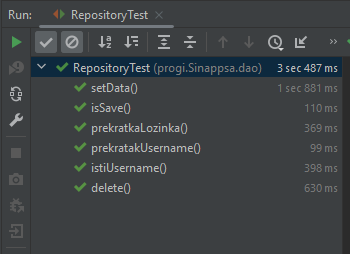
\includegraphics[scale=1]{slike/ispitivanje1.PNG} 
				\centering
				\caption{Rezultati RepositoryTest testova}
				\label{fig:RepositoryTest}
			\end{figure}
			\noindent Veoma slične testove napisali smo i za provjeru service sloja, gdje smo provjeravali KolegijService i SmjerService interface i koji također svi ispravno rade.
			
			\begin{figure}[H]
				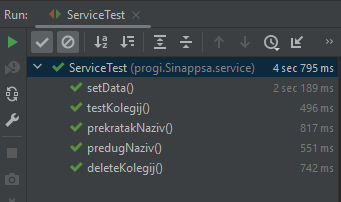
\includegraphics[scale=1]{slike/ispitivanje2.PNG} 
				\centering
				\caption{Rezultati ServiceTest testova}
				\label{fig:ServiceTest}
			\end{figure}
			
			\noindent Za provjeru controller sloja smo koristili OglasController. Na početku svakog testa zadali smo odgovarajući URL stranice, odredili vrstu HTTP zahtjeva, te postavili potrebne ulazne podatke. Za dodavanje novog oglasa najprije smo u string varijablu u JSON formatu spremili naslov, opis, idPomagaca, idKolegija i idKategorije te to postavili kao entitet zahtjeva. Nakon što se zahtjev pošalje i dobijemo odgovor provjeravamo je li se on izvršio dobro. Najprije provjeravamo je li statusLine 200, te vraća li se u odgovoru “OK” kako je i zadano u controller-u.
			
			
			\begin{verbatim}
			    @Test
			    @Order(1)
			    public void addNewOglas() throws NoSuchAlgorithmException, 
			    KeyStoreException, KeyManagementException, IOException {
			        String pageUrl ="http://localhost:8080/api/oglasi/create";
					
			        TrustStrategy acceptingTrustStrategy = (X509Certificate[] 
			        chain, String authType) -> true;
			        SSLContext sslContext = org.apache.http.ssl.SSLContexts.
			        custom().loadTrustMaterial(null, acceptingTrustStrategy)
			        .build();
			        SSLConnectionSocketFactory csf = new 
			        SSLConnectionSocketFactory(sslContext);
			        CloseableHttpClient httpClient = HttpClients.custom()
			        .setSSLSocketFactory(csf).build();
					
			        HttpPost httpPost = new HttpPost(pageUrl);
			        String JSON_STRING = "{\"naslov\":\"Oglas 
			            iz Controller testa\",\"opis\":\"Novi 
			            opis iz Controller testa\"," + "\"idPomagaca\ 
			            ":164,\"idKolegija\":140,\"idKategorije\":3}";
		            HttpEntity stringEntity = new StringEntity(JSON_STRING, 
		            ContentType.APPLICATION_JSON);
		            httpPost.setEntity(stringEntity);
					
		            CloseableHttpResponse response = httpClient.execute(httpPost);
					
		            logger.info("code={}", 
		            response.getStatusLine().getStatusCode());
		            logger.info("statusLine={}", 
		            response.getStatusLine());
		            Assertions.assertEquals(200, 
		            response.getStatusLine().getStatusCode());
		            String jsonString = 
		            EntityUtils.toString(response.getEntity());
		            logger.info("jsonString={}", jsonString);
		            Assertions.assertEquals("OK",jsonString);
			    }
			\end{verbatim}
			U ControllerTestu smo još pokušali dohvatiti sve oglase za prijavljenog korisnika kako bismo provjerili provjerava li se autorizacija na dobar način tamo gdje je ona potrebna. U header smo postavili username i password korisnika iz baze te nakon što smo dobili odgovor kojem je statusLine 200 provjeravamo počinje li odgovor sa id-om korisnika kojeg smo mu zadali.
			
			\begin{verbatim}
			    @Test
			    @Order(2)
			    public void getOglasiKorisnika() throws 
			    NoSuchAlgorithmException, KeyStoreException, 
			    KeyManagementException, IOException, JSONException {
			        //dohvati sve oglase za prijavljenog korisnika
			        String pageUrl ="http://localhost:8080/api/oglasi
			            /dohvati/korisnik";
					
			        TrustStrategy acceptingTrustStrategy = 
			        (X509Certificate[] chain, String authType) -> true;
			        SSLContext sslContext = org.apache.http.ssl
			        .SSLContexts.custom().loadTrustMaterial(null, 
			        acceptingTrustStrategy).build();
			        SSLConnectionSocketFactory csf = new 
			        SSLConnectionSocketFactory(sslContext);
		        CloseableHttpClient httpClient = HttpClients
		        .custom().setSSLSocketFactory(csf).build();
					
			        HttpGet httpGet = new HttpGet(pageUrl);
		        String auth =  username + ":" + password;
			        byte[] encodedAuth = 
			        Base64.getEncoder().encode(auth.getBytes
			        (StandardCharsets.ISO_8859_1));
			        String authHeader = "Basic " + new String(encodedAuth);
			        httpGet.setHeader(HttpHeaders.AUTHORIZATION, authHeader);
					
			        CloseableHttpResponse response = httpClient
			        .execute(httpGet);
					
		        logger.info("code={}", response.getStatusLine()
		        .getStatusCode());
			        logger.info("statusLine={}", response.getStatusLine());
			        Assertions.assertEquals(200, 
			        response.getStatusLine().getStatusCode());
			        String jsonString = EntityUtils.toString(response.getEntity());
			        logger.info("jsonString={}", jsonString);
		        Assertions.assertTrue(jsonString
		        .contains("\"id\":164,\"ime\":\"Milica\""));
			    }
			\end{verbatim}
			Controller testovi također svi rade ispravno.
			
			\begin{figure}[H]
				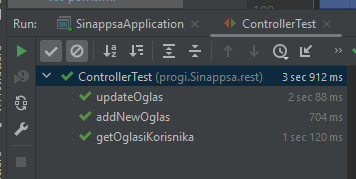
\includegraphics[scale=1]{slike/ispitivanje3.PNG} 
				\centering
				\caption{Rezultati ControllerTest testova}
				\label{fig:ControllerTest}
			\end{figure}
		
			\subsection{Ispitivanje sustava}
			
			Ispitivanje cijelog sustava napravili smo pomoću Selenium WebDrivera unutar Junit testova.
			
			\noindent Na početku imamo dva testa koja testiraju ispravnu i neispravnu prijavu. U svakom od njih naprijed definiramo postavke samo drivera, te mu zadamo URL stranice sa koje započinje test. Nakon što pronađe element u koji se upisuje username, pošaljemo mu podatke za username, te isto učinimo i za password. Budući da su podaci ispravni, aplikacija automatski preusmjerava korisnika na početnu stranicu pa se to i provjerava u posljednjem retku testa.
			
			\begin{verbatim}
			    @Test
			    public void testLogin() throws InterruptedException {
			        System.setProperty("webdriver.chrome.driver", 
			        "C:\\Program Files (x86)\\Chrome Driver\\chromedriver.exe");
			        WebDriver driver = new ChromeDriver();
			        driver.manage().timeouts().implicitlyWait(10, TimeUnit.SECONDS);
			        driver.get("https://sinappsa.netlify.app/prijava");
			        WebElement element = driver.findElement(By.name("usernameOrEmail"));
			        element.sendKeys("vmilica");
			        element = driver.findElement(By.name("password"));
			        element.sendKeys("vmilica1234");
			        driver.findElement(By.cssSelector("Button[type='submit']")).click();
			        Thread.sleep(3000);
			        String url = driver.getCurrentUrl();
			        driver.quit();
			        Assertions.assertEquals("https://sinappsa.netlify.app/", url);
		    }
			\end{verbatim}
			Test za neispravnu prijavu je skoro identičan kao za ispravnu, jedino što mu se zadaju neispravni podaci. U ovom slučaju to je neispravna lozinka i on mora na samom kraju ostati na stranici za prijavu, a ne biti preusmjeren na početnu stranicu aplikacije.
			
			\begin{verbatim}
		    @Test
		    public void failLogin() throws InterruptedException {
			        System.setProperty("webdriver.chrome.driver", 
			        "C:\\Program Files (x86)\\Chrome Driver\\chromedriver.exe");
			        WebDriver driver = new ChromeDriver();
			        driver.manage().timeouts().implicitlyWait(10, TimeUnit.SECONDS);
			        driver.get("https://sinappsa.netlify.app/prijava");
			        WebElement element = driver.findElement(By.name("usernameOrEmail"));
			        element.sendKeys("vmilica");
			        element = driver.findElement(By.name("password"));
			        element.sendKeys("vmilica123456");
			        driver.findElement(By.cssSelector("Button[type='submit']")).click();
			        Thread.sleep(3000);
			        String url = driver.getCurrentUrl();
			        driver.quit();
			        Assertions.assertEquals("https://sinappsa.netlify.app/prijava", url);
			    }
			\end{verbatim}
			Testirali smo i ponaša li se aplikacija kako treba ako se ne upišu svi potrebni podaci prilikom dodavanja novog oglasa. Naravno, za dodavanje novog oglasa korisnik mora biti prijavljen, stoga na početku testa, nakon postavki drivera slijedi prijava u aplikaciju identična prvom testu. Nakon što je prijava bila uspješna na početnoj stranici odabire se gumb “Dodaj oglas” i u tražena polja upisuju se samo naslov i opis oglasa dok smjer, kolegij i kategorija ostaju prazni što aplikacija ne bi trebala podržati. Budući da je test uhvatio iznimku, vidimo da takav oglas nije dodan u bazu podataka i zaključujemo da aplikacija radi ispravno.
			
			\begin{verbatim}
			    @Test
			    void dodavanjeOglasa() throws InterruptedException {
			        //neuspjelo
			        System.setProperty("webdriver.chrome.driver", 
			        "C:\\Program Files (x86)\\Chrome Driver\\chromedriver.exe");
			        WebDriver driver = new ChromeDriver();
			        driver.manage().timeouts().implicitlyWait(10, TimeUnit.SECONDS);
			        driver.get("https://sinappsa.netlify.app/prijava");
			        WebElement element = driver.findElement(By.name("usernameOrEmail"));
			        element.sendKeys("vmilica");
			        element = driver.findElement(By.name("password"));
			        element.sendKeys("vmilica1234");
			        driver.findElement(By.cssSelector("Button[type='submit']")).click();
			        Thread.sleep(3000);
			        String url = driver.getCurrentUrl();
			        Assertions.assertEquals("https://sinappsa.netlify.app/", url);
			        driver.findElement(By.xpath("//Button[text()='Dodaj oglas']")).click();
			        element = driver.findElement(By.name("naslov"));
			        element.sendKeys("Selenium naslov oglasa");
			        element = driver.findElement(By.name("opis"));
			        element.sendKeys("Selenium opis novog oglasa");
			        try {
			            driver.findElement(By.xpath("//Button[text()='Potvrdi']")).click();
			        } catch (Exception e) {}
			        System.out.println("Uhvatio sam iznimku!!");
			        driver.findElement(By.xpath("//button[text()='Ok']")).click();
			        Assertions.assertEquals("https://sinappsa.netlify.app/", url);
			        driver.quit();
			    }
			\end{verbatim}
			Posljednji test sustava provjerava javljanje na upite već postavljenih oglasa. Također se ni na upite ne može javljati korisnik koji nije prijavljen, stoga najprije moramo provesti valjanu prijavu. Nakon što je prijava uspjela, a to vidimo preusmjeravanjem na početnu stranicu, odabiremo oglas koji nije naš i na koji se ranije nismo javili, upisujemo poruku korisniku koji je oglas objavio i šaljemo upit.
			
			\begin{verbatim}
			    @Test
		    void dodavanjeUpita() throws InterruptedException {
			        //nije uspjelo
			        System.setProperty("webdriver.chrome.driver", 
			        "C:\\Program Files (x86)\\Chrome Driver\\chromedriver.exe");
			        WebDriver driver = new ChromeDriver();
			        driver.manage().timeouts().implicitlyWait(10, TimeUnit.SECONDS);
		            driver.get("https://sinappsa.netlify.app/prijava");
			        WebElement element = driver.findElement(By.name("usernameOrEmail"));
			        element.sendKeys("vmilica");
			        element = driver.findElement(By.name("password"));
			        element.sendKeys("vmilica1234");
			        driver.findElement(By.cssSelector("Button[type='submit']")).click();
			        Thread.sleep(3000);
			        String url = driver.getCurrentUrl();
			        Assertions.assertEquals("https://sinappsa.netlify.app/", url);
			        Thread.sleep(3000);
			        driver.findElement(By.xpath("//button[text()='Javi se']")).click();
			        element = driver.findElement(By.xpath("//textarea"));
			        element.sendKeys("Javljam se na ovaj upit iz Seleniuma!");
                    driver.findElement(By.xpath("//button[text()='Submit']")).click();
			        driver.quit();
			    }
			\end{verbatim}
			Nakon pokretanja svih testova sustava vidimo da i oni ispravno rade.
			
			\begin{figure}[H]
				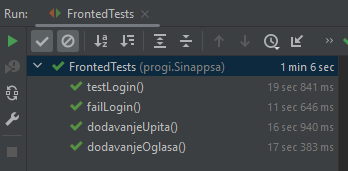
\includegraphics[scale=1]{slike/ispitivanje4.PNG} 
				\centering
				\caption{Rezultati testova sustava}
				\label{fig:FrontendTest}
			\end{figure}
			
			\eject 
		
		
		\section{Dijagram razmještaja}
			Dijagram razmještaja je strukturni statički UML dijagram koji opisuje topologiju sustava i usredotočen je na odnos sklopovskih i programskih dijelova. Na klijentskoj strani je PC računalo na kojem je pokrenut web preglednik. Klijent se protokolom HTTPS spaja na poslužitelja. Web poslužitelj i poslužitelj baze podataka nalaze se na istom računalu. Sustav je baziran na arhitekturi „klijent – poslužitelj“.
			
			\begin{figure}[H]
				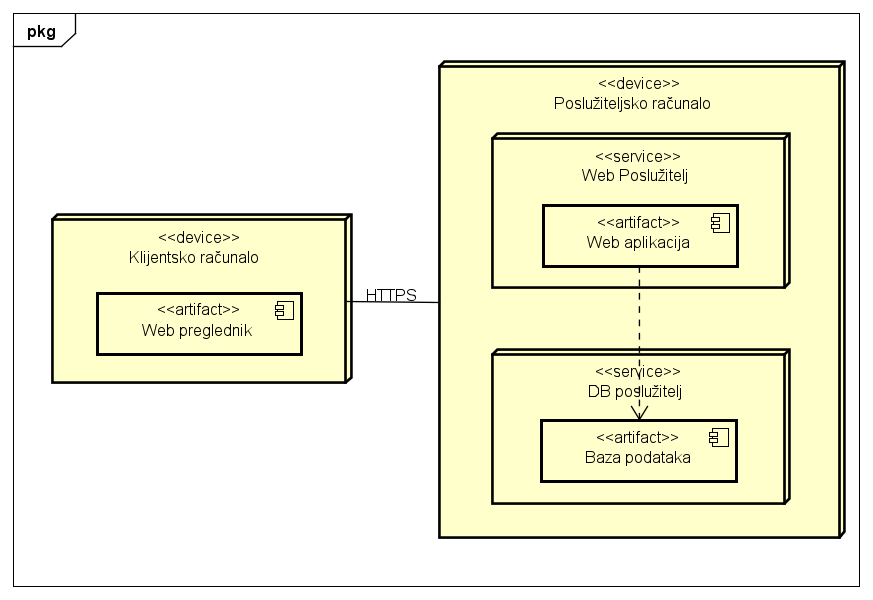
\includegraphics[scale=0.65]{dijagrami/DijagramRazmjestaja.png}
				\centering
				\caption{Dijagram razmještaja}
				\label{fig:dijagram razmjestaja}
			\end{figure}

			\eject 
		
		\section{Upute za puštanje u pogon}
			\noindent \textbf{Instalacija poslužitelja baze podataka}
			
			Na poslužitelju Render potrebno je napraviti poslužitelj baze podataka. Odabirom \textit{New} -$>$ \textit{PostgreSQL} radi se nova SQL baza. Potrebno je unijeti sljedeće podatke:
			\begin{packed_item}
				\item Ime: ime pod kojim će se baza spremati na Renderu
				\item Baza: postavljanje atributa dbname koji ćemo koristiti kod povezivanja s backend dijelom aplikacije
				\item PostgreSQL: odabir verzije PostgreSQL
			\end{packed_item}
			Opcionalno može se dodati ime korisnika (u suprotnom će se naziv korisnika slučajno generirati).
			\begin{figure}[H]
				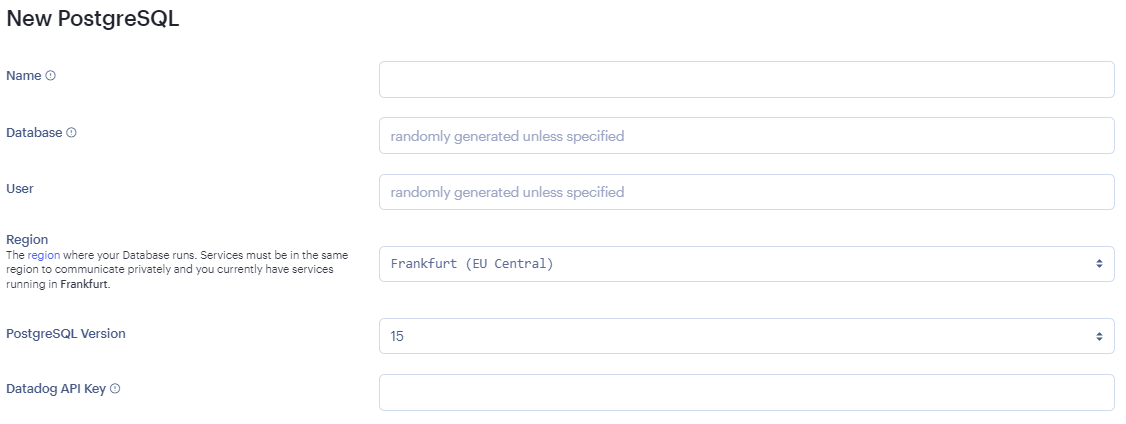
\includegraphics[scale=0.5]{slike/slika1.png}
				\centering
				\caption{Prikaz dijaloškog okvira stvaranja baze podataka}
				\label{fig:dij okvir}
			\end{figure}
			\begin{figure}[H]
				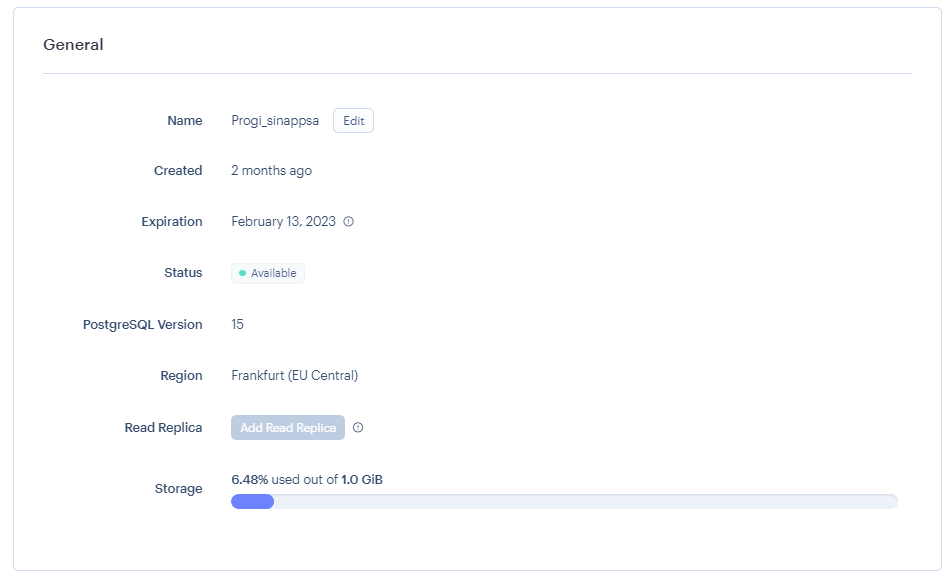
\includegraphics[scale=0.45]{slike/slika2.png}
				\centering
				\caption{Uspješno dodan poslužitelj baze podataka}
				\label{fig:uspj dodan}
			\end{figure}
			
			\noindent \textbf{Povezivanje backend dijela aplikacije s bazom podataka}
			
			U backend dijelu aplikacije, kako bismo se uspješno povezali s bazom, u Spring Boot aplikaciju u datoteku Sinappsa/src/resources/deploy/application.properties treba dodati 3 atributa:
			\begin{packed_item}
				\item spring.datasource.url 
				\item spring.datasource.username 
				\item spring.datasource.password
			\end{packed_item}
			Ove atribute treba postaviti u skladu s podacima za povezivanje na poslužitelj baze koji su dostupni na Renderu.
			\begin{figure}[H]
				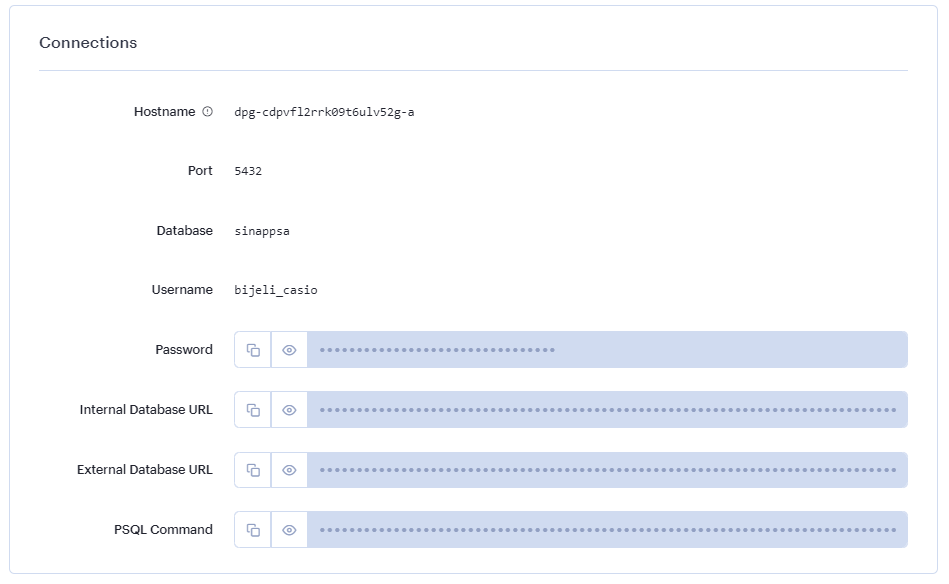
\includegraphics[scale=0.5]{slike/slika3.png}
				\centering
				\caption{Prikaz podataka potrebnih za povezivanje na poslužitelj baze podataka}
				\label{fig:povez baz pod}
			\end{figure}
			
			Atribut spring.datasource.url treba postaviti na string koji će predstavljati URL adresu poslužitelja baze podataka. Taj URL započinje sa stringom jdbc:postgresql:// te se na taj dio zalijepi \textit{Hostname} poslužitelja zajedno s portom (deafultni port je 5432) te se nakon toga doda ime baze podataka. Atribut spring.datasource.username postavlja se na \textit{Username} koji je dodijelio poslužitelj baze podataka. Atribut 
			
			\noindent spring.datasource.password poprima vrijednosti generirane zaporke koja služi za autentifikaciju pri spajanju na poslužitelj baze podataka.
			
			
			\noindent \textbf{Instalacija poslužitelja backend dijela aplikacije}
			
			Za instalaciju backend poslužitelja koristimo Render. Kako Render ne pruža podršku za Javu, prije same instalacije poslužitelja backenda potrebno je Java kod omotati u Docker izvršnu okolinu pomoću Dockerfile-a na način prikazan na slici \ref{fig:dockerfile}.
			\begin{figure}[H]
				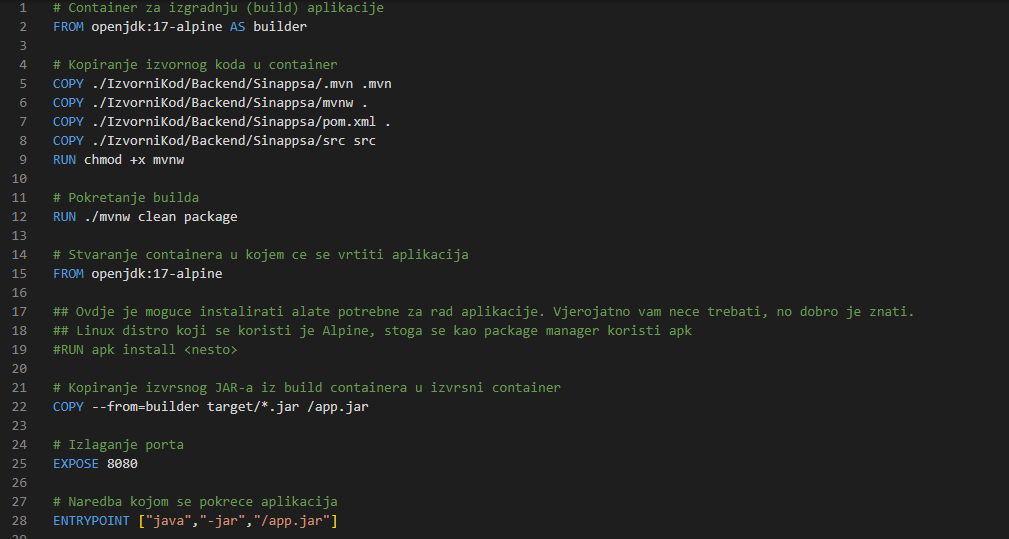
\includegraphics[scale=0.5]{slike/slika4.png}
				\centering
				\caption{Prikaz Dockerfilea}
				\label{fig:dockerfile}
			\end{figure}
			
			Kako bismo uspješno postavili poslužitelj potrebno je odabrati opciju \textit{New}-$>$\textit{Web Sevice}. Zatim se potrebno povezati sa Git repozitorijem na kojem se nalazi kod backend aplikacije. Nakon toga Render zahtjeva sljedeće parametre:
			\begin{packed_item}
				\item \textit{Name}: ime web servisa 
				\item \textit{Branch}: grana git repozitorija na kojoj se nalazi web servis 
				\item Korijenski direktorij: put do direktorija u kojem se nalazi napravljeni Dockerfile
				\item \textit{Enviroment}: odabir izvršne okoline (budući da Render nema direktnu podršku za Javu ovdje odabiremo Docker)
			\end{packed_item}
			\begin{figure}[H]
				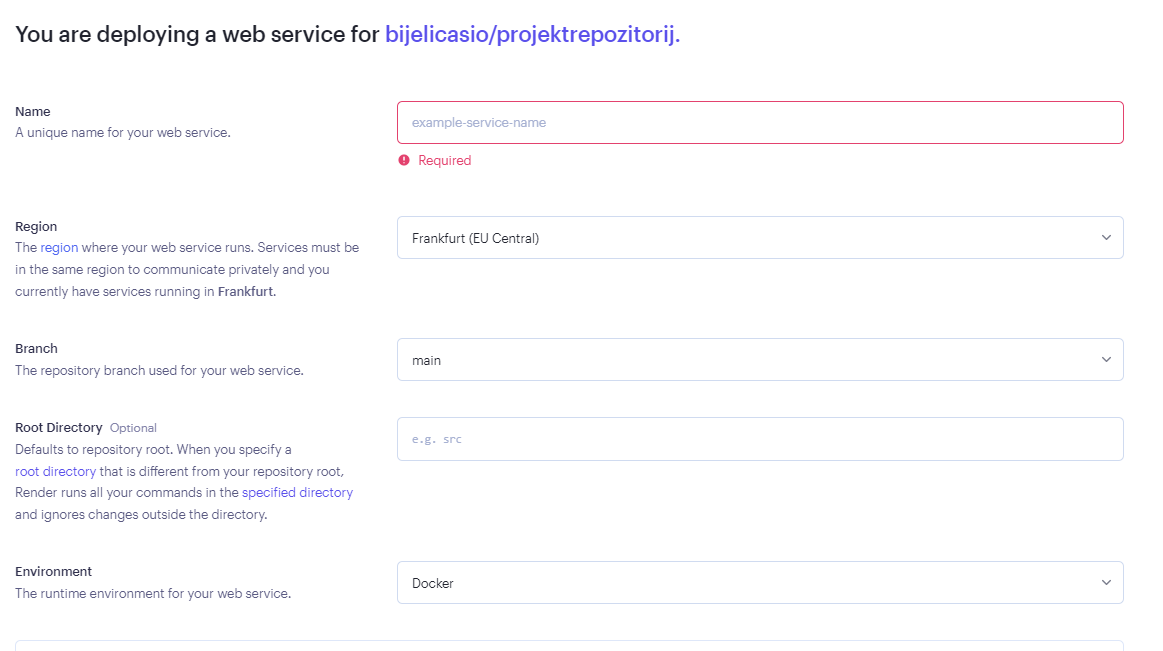
\includegraphics[scale=0.4]{slike/slika5.png}
				\centering
				\caption{Prikaz podataka potrebnih za instalaciju poslužitelja backend dijela aplikacije}
				\label{fig:backend pod}
			\end{figure}
		
			Klikom na gumb \textit{Advanced} proširuju se mogućnosti za postavljene web servisa. U \textit{Advanced} postavkama pod karticom \textit{Enviroment variables} potrebno je dodati dvije varijable izvršne okoline:
			\begin{packed_item}
				\item DB\_PASS
				\item DB\_USERNAME
			\end{packed_item}
			Ove dvije varijable postavljamo na vrijednosti \textit{usernamea} i \textit{passworda} s poslužitelja baze podataka. Odabirom opcije \textit{Create servis} započinje stvaranje servisa i stvaranje tablica u bazi podataka.
		
			
			\noindent \textbf{Pokretanje backend aplikacije i stvaranje tablica u bazi}
			
			Pokretanjem Spring Boot backend aplikacije pomoću Java Persistance API-ja koji služi za perzistenciju podataka aplikacije pomoću objektno realcijskog preslikavanja (eng. Object Relational Mapping - ORM) u povezanoj bazi podataka stvaraju se tablice iz klasa definiranih u aplikaciji koje su anotirane oznakom \textit{@Entity}. 
			
			Uspješnim deployom backend aplikacije ona postaje dostupna za rad preko interneta. Pomoću kartice \textit{Logs} na Renderu moguće je pratiti zahtjeve koji pristižu na servis te odgovore na zahtjeve i eventualne greške.
			
			
			\noindent \textbf{Instalacija poslužitelja frontenda}
			
			Za pogon frontend dijela aplikacije ne koristimo Render, već Netlify. Nakon uspješnog stvaranja tima na Netlifyu odabirom opcije \textit{Add new Site} pod kategorijom \textit{Site} možemo deployati stranicu. Nakon \textit{Add new Site} odabiremo opciju \textit{Import an existing project} te se povezemo sa Git repozitorijem. Nakon odabira repozitorija odabiremo granu u repozitoriju na kojem se nalazi izvorni kod dijela stranice i u polje \textit{Base directory} stavljamo putanju do mape u kojoj se nalazi izvorni kod. Za \textit{build command} postavljamo naredbu \textit{npm run build}. 
			\begin{figure}[H]
				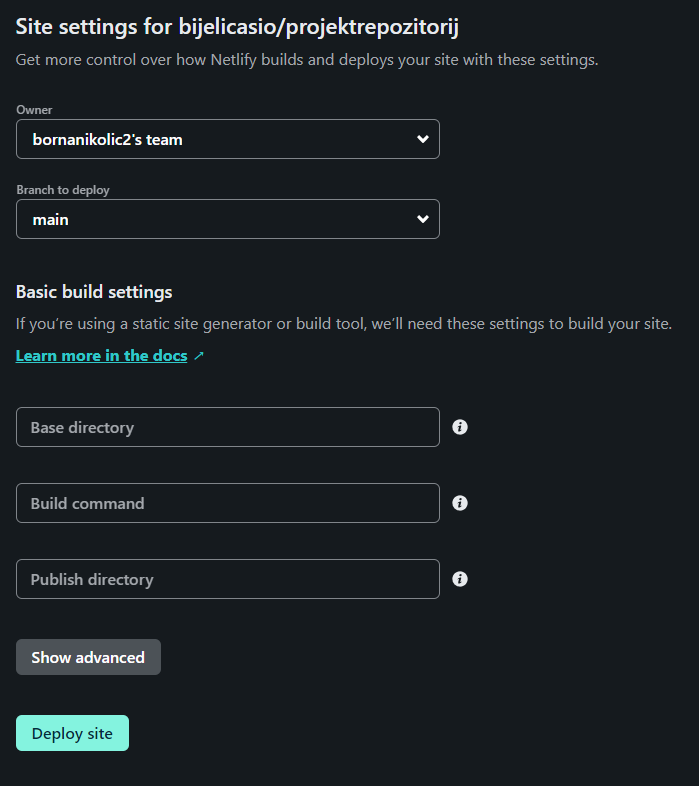
\includegraphics[scale=0.5]{slike/slika6.png}
				\centering
				\caption{Prikaz podataka potrebnih za instalaciju frontend poslužitelja}
				\label{fig:frontend pod}
			\end{figure}
			
			Odabirom opcije \textit{Deploy site} kreće se u \textit{build frontend} i po uspješnom završetku web aplikacija je puštena u pogon na javnom poslužitelju.
			\eject 
	\chapter{Zaključak i budući rad}
		Naš projektni zadatak bio je realizacija web aplikacije Sinappsa koja omogućuje studentima FER-a da traže ili pružaju pomoć vezanu za fakultet. Nakon skoro cijelog semestra rada na aplikaciji ponosno možemo reći da smo implementirali i zadovoljili sve zahtjeve radnog zadatka.
		
		Prvih sedam tjedana rada na aplikaciji išli su sporijim tempom. Prije početka samog programiranja aplikacije, proučili smo projektni zadatak, napravili obrasce uporabe te se dogovorili kako će aplikacija izgledati i od kojih komponenata će se sastojati. Zatim smo se podijelili na frontend, backend i dokumentaciju. Nakon podjele krenuli smo se upoznavati s tehnologijama s kojima je većina nas prvi put stupila u kontakt. Prije prve revizije imali smo osposobljene osnovne funkcionalnosti aplikacije, a to su bile registracija, prijava i dizajn stranice.
		
		Nakon prve revizije, u dva tjedna napravljene su gotovo sve funkcionalnosti aplikacije kako bi se mogla predati alfa inačica aplikacije. Nakon manjih prepravaka u kodu, aplikacija je bila gotova i spremna za deploy. Rad na dokumentaciji prvenstveno se sastojao od crtanja i opisivanja UML dijagrama arhitekture aplikacije. Na kraju je učinjeno ispitivanje sustava i komponenti kako bi se provjerio rad aplikacije. 
		
		Uz komunikaciju preko WhatsApp-a, skoro smo svaki tjedan imali sastanke uživo ili preko Microsoft Teamsa kako bi rasporedili zadatke za nadolazeći tjedan. Česti sastanci natjerali su nas da radimo redovito te su poticali što bolju komunikaciju među članovima tima.
		Rad na ovom projektu bio je iznimno koristan jer nam je dao uvid u stvarni svijet web developera, od dizajniranja stranice do izrade dokumentacije. Također je prikazao važnost harmonijskog rada u grupi kako bi sve bilo izrađeno i predano na vrijeme. Iako u određenim trenutcima težak, ovaj projekt je bio veoma bitan kao primjer simulacije rada u industriji.
		
		\eject 

	\chapter*{Popis literature}
		\addcontentsline{toc}{chapter}{Popis literature}
		
		\begin{enumerate}
			
			
			\item  Programsko inženjerstvo, FER ZEMRIS, \url{http://www.fer.hr/predmet/proinz}
			
			\item  I. Sommerville, "Software engineering", 8th ed, Addison Wesley, 2007.
			
			\item  T.C.Lethbridge, R.Langaniere, "Object-Oriented Software Engineering", 2nd ed. McGraw-Hill, 2005.
			
			\item  I. Marsic, Software engineering book``, Department of Electrical and Computer Engineering, Rutgers University, \url{http://www.ece.rutgers.edu/~marsic/books/SE}
			
			\item  The Unified Modeling Language, \url{https://www.uml-diagrams.org/}
			
			\item  Astah Community, \url{http://astah.net/editions/uml-new}
			
			\item  What is React.js?, \url{https://blog.hubspot.com/website/react-js}
			
			\item  What Is Spring Boot?, \url{https://stackify.com/what-is-spring-boot/}
			
			\item  Spring Boot - Architecture, \url{https://www.geeksforgeeks.org/spring-boot-architecture/}
		\end{enumerate}
	 
	
	
	\begingroup
	\renewcommand*\listfigurename{Indeks slika i dijagrama}
	%\renewcommand*\listtablename{Indeks tablica}
	%\let\clearpage\relax
	\listoffigures
	%\vspace{10mm}
	%\listoftables
	\endgroup
	\addcontentsline{toc}{chapter}{Indeks slika i dijagrama}

	\chapter*{Dodatak: Prikaz aktivnosti grupe}
		\addcontentsline{toc}{chapter}{Dodatak: Prikaz aktivnosti grupe}
		
		\section*{Dnevnik sastajanja}
		
		\begin{packed_enum}
			\item  sastanak
			
			\item[] \begin{packed_item}
				\item Datum: 20.listopada 2022.
				\item Prisustvovali: L.Majer, A.Zaja, B.Nikolić, A.Grčević, M.Majdiš, T.Margetić, M.Pavičić, M.Petričević, M.Vuković
				\item Teme sastanka:
				\begin{packed_item}
					\item  pojašnjenje dobivenog zadatka
				\end{packed_item}
			\end{packed_item}
			
		
			\item sastanak
			
				\item[] \begin{packed_item}
				\item Datum: 31.listopada 2022.
				\item Prisustvovali: B.Nikolić, A.Grčević, M.Majdiš, T.Margetić, M.Pavičić, M.Petričević, M.Vuković
				\item Teme sastanka:
				\begin{packed_item}
					\item  podjela zadataka
					\item dogovor oko korištenih tehnologija
					\item skiciranje izgleda stranice
				\end{packed_item}
			\end{packed_item}
		
		
			\item sastanak
				
				\item[] \begin{packed_item}
					\item Datum: 3.studenoga 2022.
					\item Prisustvovali: L.Majer, B.Nikolić, A.Grčević, M.Pavičić
					\item Teme sastanka:
					\begin{packed_item}
						\item ispravak sekvencijskih dijagrama
						\item ispravak baze podataka
						\item objašnjenje nejasnoća
					\end{packed_item}
				\end{packed_item}
			
			
			\item sastanak
			
				\item[] \begin{packed_item}
					\item Datum: 9.studenoga 2022.
					\item Prisustvovali: B.Nikolić, A.Grčević, M.Majdiš, T.Margetić, M.Pavičić, M.Petričević, M.Vuković
					\item Teme sastanka:
					\begin{packed_item}
						\item pregled napravljene stranice
						\item raspodjela daljnjih zadataka
					\end{packed_item}
				\end{packed_item}
			
		
			\item sastanak
			
			\item[] \begin{packed_item}
				\item Datum: 12.prosinca 2022.
				\item Prisustvovali: B.Nikolić, M.Majdiš, T.Margetić, M.Pavičić, M.Vuković
				\item Teme sastanka:
				\begin{packed_item}
					\item rješavanje problema spajanja s bazom
					\item raspodjela daljnjih zadataka
				\end{packed_item}
			\end{packed_item}
		
			
			\item sastanak
			
			\item[] \begin{packed_item}
				\item Datum: 15.prosinca 2022.
				\item Prisustvovali: B.Nikolić, M.Majdiš, T.Margetić, M.Petričević, M.Vuković
				\item Teme sastanka:
				\begin{packed_item}
					\item dogovor oko testiranja i završnih rokova
					\item raspodjela daljnjih zadataka
				\end{packed_item}
			\end{packed_item}
		
			
			\item sastanak
			
			\item[] \begin{packed_item}
				\item Datum: 2.siječnja 2023.
				\item Prisustvovali: B.Nikolić, A.Grčević, M.Majdiš, T.Margetić, M.Petričević, M.Vuković
				\item Teme sastanka:
				\begin{packed_item}
					\item prezentacije napisanih kodova
					\item raspodjela daljnjih zadataka
				\end{packed_item}
			\end{packed_item}
		
			\item sastanak
			
			\item[] \begin{packed_item}
				\item Datum: 7.siječnja 2023.
				\item Prisustvovali: B.Nikolić, A.Grčević
				\item Teme sastanka:
				\begin{packed_item}
					\item pisanje projektne dokumentacije
				\end{packed_item}
			\end{packed_item}
		
		\end{packed_enum}
	
		\eject
		
		\section*{Tablica aktivnosti}
		
		\begin{longtblr}[
			label=none,
			]{
				vlines,hlines,
				width = \textwidth,
				colspec={X[7, l]X[1, c]X[1, c]X[1, c]X[1, c]X[1, c]X[1, c]X[1, c]}, 
				vline{1} = {1}{text=\clap{}},
				hline{1} = {1}{text=\clap{}},
				rowhead = 1,
			} 
			{} & {\rotatebox{90}{\textbf{Borna Nikolić}}} & {\rotatebox{90}{\textbf{Ana Grčević }}} &	{\rotatebox{90}{\textbf{Martina Majdiš }}} & {\rotatebox{90}{\textbf{Tin Margetić }}} &	{\rotatebox{90}{\textbf{Matija Pavičić }}} & {\rotatebox{90}{\textbf{Mihael Petričević }}} &	{\rotatebox{90}{\textbf{Milica Vuković }}} \\  
			Upravljanje projektom 		& 16h &  &  &  &  & 4h & \\ 
			Opis projektnog zadatka 	&  & 3.5h &  &  &  &  & \\ 
			
			Funkcionalni zahtjevi       & 10h & 2h &  & 3h & 2h & 3h &  \\ 
			Opis pojedinih obrazaca 	&  & 1h &  &  &  &  &   \\ 
			Dijagram obrazaca 			& 4h & 2.5h & 1.5h & 1.5h & 1.5h & 1.5h & 1h \\ 
			Sekvencijski dijagrami 		& 8h & 3h & 2h & 2h & 2h & 2h &  \\ 
			Opis ostalih zahtjeva 		&  & 0.2h &  &  &  &  & 0.5h \\ 
			
			Arhitektura i dizajn sustava	 &  & 4.5h &  &  &  &  &  \\ 
			Baza podataka				& 3h &  &  &  &  &  &   \\ 
			Dijagram razreda 			& 3.5h & 1h &  &  &  &  &   \\ 
			Dijagram stanja				&  & 1.5h &  &  &  &  &  \\ 
			Dijagram aktivnosti 		&  & 2h &  &  &  &  &  \\ 
			Dijagram komponenti			& 1.5h &  &  &  &  &  &  \\ 
			Korištene tehnologije i alati 		&  & 2h &  &  &  &  &  \\ 
			Ispitivanje programskog rješenja 	&  & 1h &  &  &  &  & 1h \\ 
			Dijagram razmještaja			&  & 1h &  &  &  &  &  \\ 
			Upute za puštanje u pogon 		& 1.5h & 1h &  &  &  &  &  \\  
			Dnevnik sastajanja 			&  & 0.5h &  &  &  &  &  \\ 
			Zaključak i budući rad 		&  & 1h &  &  &  &  &  \\  
			Popis literature 			&  & 0.5h &  &  &  &  &  \\  
			&  &  &  &  &  &  &  \\ \hline 

			\textit{izrada početne stranice} 				&  &  &  & 6h &  & 3h &  \\  
			\textit{izrada registracijske stranice} 		&  &  &  & 5h &  & 3h &  \\ 
			\textit{registracija (avatar ikone)} 			&  &  &  &  &  & 3h &  \\ 
				\textit{izrada login stranice} 				&  &  &  & 4h &  & 3h &  \\  
			\textit{izrada baze podataka} 		 			& 12h &  &  &  &  &  & \\  
			\textit{spajanje s bazom podataka} 				&  &  &  &  &  & 23h &  \\ 
			\textit{back end} 								&  &  & 30h &  & 25h & 19h & 10h \\  
			\textit{deploy baze podataka} 					& 4.5h &  &  &  &  &  &  \\  
			\textit{deploy front enda i back enda} 			& 17.5h &  &  &  &  & 4h &  \\  
			\textit{ispitivanje programskog rješenja} 		&  &  &  &  &  &  & 20h \\ 
			\textit{izrada profil stranice} 				&  &  &  &  &  & 5h &  \\ 
			\textit{izrada forme za dodavanje oglasa}		&  &  &  & 3h &  &  &  \\
			\textit{izrada admin stranice}	 				&  &  &  & 5h &  &  &  \\  
			&  &  &  &  &  &  &\\ 
		\end{longtblr}
					
					
		\eject
		
		
		\section*{Dijagrami pregleda promjena}
		\begin{figure}[H]
			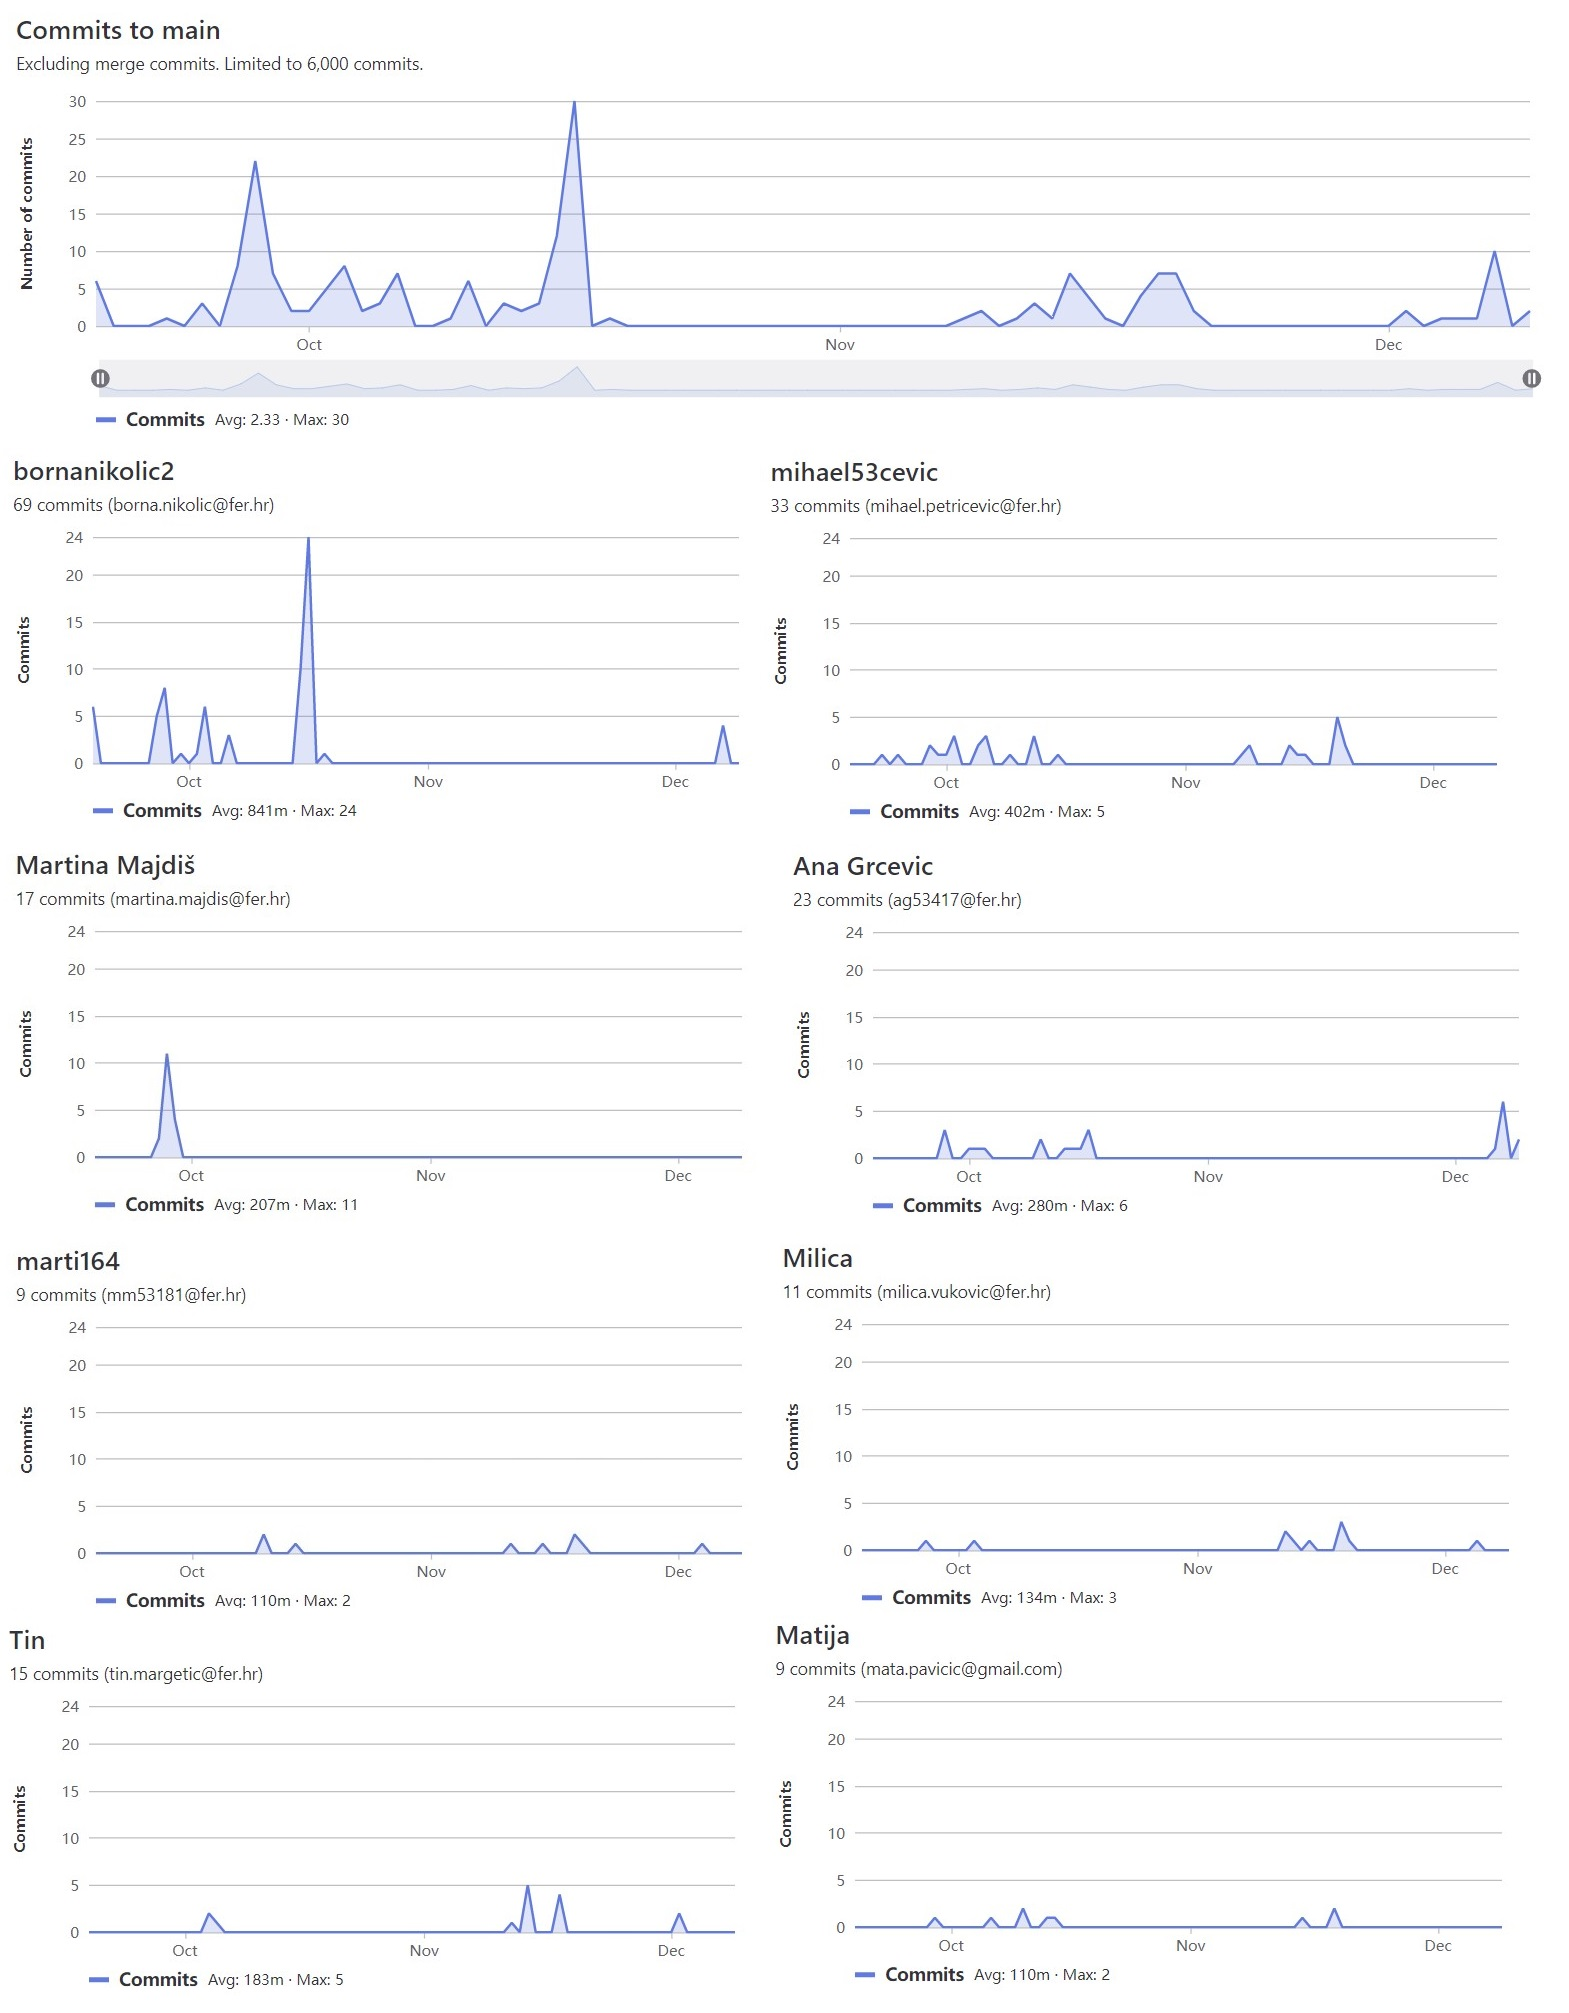
\includegraphics[scale=0.45]{dijagrami/commitovi.jpg} 
			\centering
			\caption{Prikaz aktivnosti na repozitoriju}
			\label{fig:commitovi}
		\end{figure}

		
	
	
	\eject 
		



\end{document} %naredbe i tekst nakon ove naredbe ne ulaze u izgrađen dokument 


